\documentclass[graybox, envcountchap]{svmult}
% Springer document settings
\usepackage[bottom]{footmisc}% places footnotes at page bottom

\usepackage{newtxtext}       % 
\usepackage[varvw]{newtxmath}       % selects Times Roman as basic font
%%%%%%%%%%%%%%%%%%%%%%%%%%%%%%%

% \usepackage{amssymb}
\usepackage{ntheorem}
\usepackage{amsmath}
\usepackage{enumitem}


\usepackage{graphicx}
\usepackage{color}
\usepackage{cite}
\usepackage{makeidx}


\usepackage{ascmac}
\usepackage{eclbkbox}
\usepackage{dsfont}

\usepackage{longtable}

\usepackage{url}

\usepackage{hyperref}

\usepackage{multicol}

%% --川口追加--
\makeatletter
\let\MYcaption\@makecaption
\makeatother
\usepackage{subcaption}
\captionsetup{compatibility=false}      % 必要に応じて

\makeatletter
\let\@makecaption\MYcaption
\makeatother
% ----

%%
\theoremstyle{plain}
\theoremheaderfont{\bfseries}
\theorembodyfont{\rmfamily}
\theoremseparator{\hspace{1ex}}
\theoremindent0cm
\theoremnumbering{arabic}
\theoremprework{\vspace{1ex}\begin{shadebox}\vspace{1ex}}
\theorempostwork{\vspace{-1ex}\end{shadebox}\vspace{1ex}}

%%
\theoremclass{theorem}

%%
\theoremclass{theorem}

%%
\theoremclass{theorem}


%%
\theoremstyle{break}
\theoremheaderfont{\bfseries}
\theorembodyfont{\rmfamily}
\theoremseparator{}
\theoremindent0cm
\theoremnumbering{arabic}
\theoremprework{\vspace{1.5ex}\begin{breakbox}\vspace{-0.5ex}}
\theorempostwork{\vspace{-0.5ex}\end{breakbox}\vspace{1.5ex}}

%%
\theoremstyle{nonumberplain}
\theoremseparator{\hspace{1ex}}

%%
\newtheorem{assumption}{Assumption}[section]

%%
\renewcommand{\theproblem}{}

\renewcommand{\theremark}{}


\newcommand{\red}[1]{{\color{red}#1}}
\newcommand{\blue}[1]{{\color{blue}#1}}
\newcommand{\green}[1]{{\color{green}#1}}

\DeclareMathOperator*{\argmax}{arg\,max}

\newcommand{\bm}[1]{\boldsymbol{#1}}
\newcommand{\sfT}{\mathsf{T}}

\newcommand{\advanced}{$^{\ddag}$}

\DeclareMathOperator{\sfsin}{\mathsf{sin}}
\DeclareMathOperator{\sfcos}{\mathsf{cos}}
\DeclareMathOperator{\sftan}{\mathsf{tan}}
\DeclareMathOperator{\sfarctan}{\mathsf{arctan}}

\DeclareMathOperator{\sfdiag}{\mathsf{diag}}
\DeclareMathOperator{\sfcol}{\mathsf{col}}
\DeclareMathOperator{\sfdet}{\mathsf{det}}
\DeclareMathOperator{\sfadj}{\mathsf{adj}}
\DeclareMathOperator{\sftrace}{\mathsf{trace}}

\DeclareMathOperator{\real}{\mathsf{Re}}

\DeclareMathOperator{\sfker}{\mathsf{ker}}
\DeclareMathOperator{\sfim}{\mathsf{im}}

\DeclareMathOperator{\sfdim}{\mathsf{dim}}
\DeclareMathOperator{\sfspan}{\mathsf{span}}

\DeclareMathOperator{\sfint}{\mathsf{int}}

\DeclareMathOperator*{\sfmin}{\mathsf{min}}
\DeclareMathOperator*{\sfmax}{\mathsf{max}}
\DeclareMathOperator*{\sfsup}{\mathsf{sup}}

\DeclareMathOperator{\sfsat}{\mathsf{sat}}

\newcommand{\mat}[1]{\left[\: \begin{matrix} #1 \end{matrix} \:\right]}
\newcommand{\spliteq}[1]{\begin{split} #1 \end{split}}
\newcommand{\simode}[1]{\begin{cases}  \begin{split} #1 \end{split} \end{cases}}

\newcommand{\proofend}{\hfill \rule{2mm}{3mm}}

\newcommand{\Xti}{X_i'}
\newcommand{\Xsi}{X_i}

\newcommand{\Xtone}{X_1'}
\newcommand{\XtN}{X_N'}

\newcommand{\Xt}{X'}
\newcommand{\Xs}{X}

\newcommand{\taudi}{\tau_i}
\newcommand{\taud}{\tau}

\newcommand{\Cgi}{b_i}


\newcommand{\Ifd}{I_{\rm field} }

\newcommand{\matlab}{\textsc{Matlab} }





%% --川口追加--
\newcommand{\thshift}{\theta_{12}}
\newcommand{\thshiftb}{\theta_{32}}
\newcommand{\Ysa}{\bm y_{12}}
\newcommand{\bca}{c_{12}}
\newcommand{\Ysb}{\bm y_{32}}
\newcommand{\bcb}{c_{32}}
\newcommand{\bcij}{c_{ij}}
\newcommand{\Is}{{\bm I}_{12}' }
\newcommand{\im}{\bm j}
\newcommand{\tr}{{\sf T}}

%%%%%%%%%%%%%%%%%%%%%%%%% code lines %%%%%%%%%%%%%%%%%%%%%%%%%%%%%%%%%%%%%%%%%%
\usepackage{listings}
\usepackage{xcolor}
\renewcommand{\lstlistingname}{Program}% Listing -> Algorithm
\renewcommand{\lstlistlistingname}{List of \lstlistingname s}% List of Listings -> List of Algorithms

\definecolor{codegreen}{rgb}{0,0.6,0}
\definecolor{codegray}{rgb}{0.5,0.5,0.5}
\definecolor{codepurple}{rgb}{0.58,0,0.82}
\definecolor{backcolour}{rgb}{0.95,0.95,0.92}

\lstdefinestyle{mystyle}{
    backgroundcolor=\color{backcolour},   
    commentstyle=\color{codegreen},
    keywordstyle=\color{magenta},
    numberstyle=\tiny\color{codegray},
    stringstyle=\color{codepurple},
    basicstyle=\ttfamily\footnotesize,
    breakatwhitespace=false,         
    breaklines=true,                 
    captionpos=b,                    
    keepspaces=true,                 
    numbers=left,                    
    numbersep=5pt,                  
    showspaces=false,                
    showstringspaces=false,
    showtabs=false,                  
    tabsize=2
}

\lstset{style=mystyle}

\begin{document}


\chapter{Steady-state stability analysis of power system
models}\label{sec:staana}

In this Chapter, we conduct stability analysis based on the approximate
linearization of power system models. The structure of this Chapter is as
follows. First, in Section \ref{sec:stalin}, we derive a linear approximation
model for the power system model described by a system of ordinary differential
equations using Kron reduction of the generator buses. Then, in Section
\ref{sec:numlinsta}, we explain the method for numerically analyzing the
stability of the derived linear approximation model. We also confirm through
numerical simulation that the stability of the linear approximation model
depends not only on the physical constants of the generators, loads, and
transmission lines, but also on the selection of the steady-state power flow.
Additionally, in Section \ref{sec:linmathana}, we explore advanced topics and
demonstrate how the stability of the linear approximation model can be analyzed
using the concept of passivity in dynamic systems.

\begin{COLUMN}
\noindent \textbf{Derivation of the approximate linear system}:

Consider the nonlinear system:

\begin{equation*}
  \dot{x}(t) = f\bigl(x(t)\bigr) + Bu(t) 
\end{equation*}
where $f(0)=0$. The function $f(x)$ can be expressed near the origin by a Taylor
expansion as:

\[
  f(x)=f(0) + \frac{\partial f}{\partial x} (0) x + \mbox{Second or higher order term}
\]

Here, $f(x)$ and $x$ are expressed as $f_i(x)$ and $x_i$, respectively, and
$\tfrac{\partial f}{\partial x}(x)$ is the \emph{Jacobian matrix} with the
$(i,j)$ element given by $\tfrac{\partial f_i}{\partial x_j}(x)$. By using this
Jacobian matrix, we define:

\[
  A:=\frac{\partial f}{\partial x} (0)
\]

Then, when the magnitudes of the state $x(t)$ and input $u(t)$ are sufficiently
small, the behavior of the nonlinear system can be approximated by the behavior
of the linear system obtained by neglecting terms of degree 2 or higher in the
function $f$:

\begin{equation*}
  \dot{x}^{\rm lin}(t) = Ax^{\rm lin}(t) + Bu^{\rm lin}(t) 
\end{equation*}

Note that even if $u(t)$ and $u^{\rm lin}(t)$ are the same, the state $x(t)$ of
the nonlinear system and the state $x^{\rm lin}(t)$ of the approximate linear
system may not be exactly the same.
\end{COLUMN}

\section{Stability analysis based on linear approximation}\label{sec:stalin}

\subsection{Approximate linearization of the power system
model}\label{sec:linaproxt}

In this section, we derive an approximate linear model for the power system
model where each bus has a generator connected, which is equivalent to the
Kron-reduced differential equation system model discussed in Section
\ref{sec:allgen}. We derive the approximate linear model for the steady-state
flow state. The differential equation system model is given by:

\begin{equation}\label{eq:krondyn_}
  \simode{
    \dot{\delta}_i&= \omega_0  \Delta \omega_i\\
    M_i   \Delta \dot{\omega}_i&= %\textstyle
    - D_i \Delta\omega_i   
    - f_i \left( \delta,E \right)
    +P_{{\rm mech}i}
    \\
    \taudi \dot{E}_i & = %\textstyle
    -  \tfrac{ \Xsi }{ \Xti }  E_i  + \left(
    \Xsi - \Xti
    \right)
    g_i \left( \delta,E \right)
    + V_{{\rm field}i}
  }
  \qquad
  i \in \mathcal{I}_{\rm G}
\end{equation}

However, $\delta$ and $E$ are vectors obtained by vertically arranging
$\delta_i$ and $E_i$, respectively. The nonlinear terms representing the
interactions between generators are expressed as follows:

\begin{equation}\label{eq:figi}
  \spliteq{
    f_i \left( \delta,E \right) &:=
    -E_i \sum_{j=1}^{N}
    E_j 
    \bigl(
    B_{ij}^{\rm red}
    \sfsin \delta_{ij}
    -
    G_{ij}^{\rm red}
    \sfcos \delta_{ij}
    \bigr), \\
    g_i \left( \delta,E \right) &:=
    -
    \sum_{j=1}^{N}
    E_j \bigl(
    B_{ij}^{\rm red}
    \sfcos \delta_{ij}
    +
    G_{ij}^{\rm red}
    \sfsin \delta_{ij}
    \bigr)
  }
\end{equation}

In addition, $\delta_{ij}:= \delta_i - \delta_j$ is defined. Note that, due to
the properties of reduced admittance, the reduced conductance and reduced
susceptance satisfy the symmetry condition:

\[
  G_{ij}^{\rm red}=G_{ji}^{\rm red}, \qquad 
  B_{ij}^{\rm red}=B_{ji}^{\rm red}, \qquad
  \forall (i, j) \in \mathcal{I}_{\rm G} \times \mathcal{I}_{\rm G}
\]

To obtain the partial derivatives of these nonlinear functions with respect to
each variable, we define:

\begin{equation}\label{eq:defkh}
  \spliteq{
    k_{ij}(\delta_{ij}) & :=
    -B_{ij}^{\rm red}
    \sfcos \delta_{ij}
    -
    G_{ij}^{\rm red}
    \sfsin \delta_{ij},
    \\
    h_{ij}(\delta_{ij}) &:= 
    -B_{ij}^{\rm red}
    \sfsin \delta_{ij} 
    +
    G_{ij}^{\rm red}
    \sfcos \delta_{ij}
  }
\end{equation}

Then, for $f_i$, we obtain:

\begin{equation}
  \spliteq{
    \frac{\partial f_i}{\partial \delta_i} &= 
    E_i \sum_{j=1,j\neq i}^{N} E_j k_{ij}(\delta_{ij}), \\
    \frac{\partial f_i}{\partial \delta_j} &=
    - E_i  E_j k_{ij}(\delta_{ij}),
  }
  \quad
  \spliteq{
    \frac{\partial f_i}{\partial E_i} &=
    2E_i h_{ii}(\delta_{ii})   +
    \sum_{j=1,j\neq i}^{N}
    E_j h_{ij}(\delta_{ij}), \\
    \frac{\partial f_i}{\partial E_j} &=
    E_i h_{ij}(\delta_{ij})
  }
\end{equation}
where $j \neq i$.

Similarly, we can obtain the partial derivatives of $g_i$ as follows:

\begin{equation}
  \spliteq{
    \frac{\partial g_i}{\partial \delta_i} &= 
    - \sum_{j=1,j\neq i}^{N} E_j h_{ij}(\delta_{ij}), 
    \\
    \frac{\partial g_i}{\partial \delta_j} &=
    E_j h_{ij}(\delta_{ij}),
  }
  \quad
  \spliteq{
    \frac{\partial g_i}{\partial E_i} &=
    k_{ii}(\delta_{ii}) , 
    \\
    \frac{\partial g_i}{\partial E_j} &=
    k_{ij}(\delta_{ij})
  }
\end{equation}

We denote the steady-state values of the internal state of generator $i$ as
$(\delta_{i}^{\star},E^{\star}_i)$ and the steady-state values of external
inputs as $(P_{{\rm mech}i}^{\star},V_{{\rm field}i}^{\star})$ for the
differential equation system in equation \ref{eq:krondyn_}. Furthermore, we use
symbols without the subscript $i$ to represent the vector of these values for
all $i \in \mathcal{I}_{\rm G}$. For example, $\delta^{\star}$ denotes the
vector $(\delta_i^{\star})_{i \in \mathcal{I}_{\rm G} }$. With these
steady-state values, we can write the following system of equations:

\begin{equation}\label{eq:kronss}
  \simode{
    0 &= %\textstyle
    - f_i \left( \delta^{\star} , E^{\star}  \right)
    +P_{{\rm mech}i}^{\star}
    \\
    0& = %\textstyle
    -  \tfrac{ \Xsi }{ \Xti }  E_i^{\star}  + \left(
    \Xsi - \Xti
    \right)
    g_i \left( \delta^{\star} ,E^{\star} \right)
    + V_{{\rm field}i}^{\star}
  }
  \qquad
  i \in \mathcal{I}_{\rm G}
\end{equation}

Here, note that we assume the steady-state value of the frequency deviation
$\Delta \omega_i$ in Eq. \ref{eq:krondyn_} is zero for all $i \in
\mathcal{I}_{\rm G}$. The validity of Eq. \ref{eq:kronss} corresponds to setting
the steady-state values of the external input $(P_{{\rm mech}}^{\star},V_{{\rm
field}}^{\star})$ to appropriate values that achieve supply-demand balance. By
linearizing the system around this steady state, the approximate linear model is
obtained as:

\begin{equation}\label{eq:lindyn}
  \mat{
    \dot{\delta}^{\rm lin} \\
    M \Delta \dot{\omega}^{\rm lin} \\
    \taud \dot{E}^{\rm lin}
  }
  =
  \mat{
    0 & \omega_0 I & 0\\
    -L & -D & -C \\
    B & 0 & A
  }
  \mat{
    \delta^{\rm lin} \\
    \Delta \omega^{\rm lin} \\
    E^{\rm lin}
  }
  +
  \mat{
    0 & 0 \\
    I & 0 \\
    0 & I \\
  }
  \mat{
    P_{{\rm mech}}^{\rm lin} \\
    V_{{\rm field}}^{\rm lin}
  }
\end{equation}

Note that the state and input variables with the subscript "$\rm{lin}$" are
vectors consisting of small deviations from the corresponding variables with
their steady-state values as the reference. Also,

\[
  M:=\sfdiag \left(M_i\right)_{i \in \mathcal{I}_{\rm G} }, \qquad
  D:=\sfdiag(D_i)_{i \in \mathcal{I}_{\rm G} }, \qquad
  \taud :=\sfdiag \left( \taudi \right)_{i \in \mathcal{I}_{\rm G} }
\]
are diagonal matrices where $\sfdiag(\cdot)$ is an operator that creates a
diagonal matrix from a vector.

Furthermore, for the functions $k_{ij}$ and $h_{ij}$ defined in Equation
\ref{eq:defkh}, the $(i,j)$ element of the matrices $\hat{L}$, $\hat{A}$,
$\hat{B}$, and $\hat{C}$, defined as:

\begin{equation*}
  \spliteq{
  \hat{L}_{ij} & := \left\{
  \begin{array}{cl}
  E_i^{\star} \sum_{j=1, j\neq i}^{N} 
  E_j^{\star} k_{ij}(\delta_{ij}^{\star}), & \quad i=j \\
  -E_i^{\star} E_j^{\star} k_{ij}(\delta_{ij}^{\star}), & \quad i\neq j
  \end{array}
  \right.  \\
  \hat{A}_{ij} &:=  
  \left\{
  \begin{array}{cl}
  k_{ii}(\delta_{ii}^{\star}) - 
  \tfrac{ \Xsi }{ \Xti ( \Xsi- \Xti )}, & \quad i=j \\
  k_{ij}(\delta_{ij}^{\star}), & \quad i\neq j
  \end{array}
  \right.
  \\
  \hat{B}_{ij}  &:= \left\{
  \begin{array}{cl}
  -\sum_{j=1, j\neq i}^{N} 
  E_j^{\star} h_{ij}(\delta_{ij}^{\star}), &\quad i=j \\
  E_j^{\star} h_{ij}(\delta_{ij}^{\star}), & \quad i\neq j
  \end{array}
  \right. \\
  \hat{C}_{ij} &:= \left\{
  \begin{array}{cl}
  \sum_{j=1, j\neq i}^{N} 
  E_j^{\star} h_{ij}(\delta_{ij}^{\star}), & \quad i=j \\
  E_i^{\star} h_{ij}(\delta_{ij}^{\star}), & \quad i\neq j
  \end{array}
  \right.
  }
\end{equation*}

The matrices $L$, $A$, $B$, and $C$ are then defined as follows:

\begin{equation}\label{eq:sysmats}
  \spliteq{
    L&:=\hat{L}, \\
    A&:= \sfdiag \left( \Xsi - \Xti \right)_{i \in \mathcal{I}_{\rm G} } \hat{A},  \\
    B&:= \sfdiag \left( \Xsi - \Xti \right)_{i \in \mathcal{I}_{\rm G} } \hat{B},  \\
    C&:= \sfdiag \bigl( 2E_i^{\star}h_{ii}(\delta_{ii}^{\star}) \bigr)_{i \in \mathcal{I}_{\rm G} }+ \hat{C} 
  }
\end{equation}

Note that $\delta_{ij}^{\star}:=\delta_{i}^{\star}-\delta_{j}^{\star}$. It
should be noted that the system matrix $(L,A,B,C)$ is a function of the
steady-state values $(\delta^{\star},E^{\star})$. The block diagram of this
approximate linear model is shown in Figure \ref{fig:blocklinsys}. Here, $P^{\rm
lin}$ represents the approximately linearized active power supplied by the
generators. Note that generally $\Xsi > \Xti$ for all $i$.

In power system engineering, the value obtained by differentiating the
generator's active power with respect to the rotor angle at the steady-state is
called the \textbf{synchronizing power coefficient}\index{synchronizing power
coefficient} \cite[Section 8.4]{kato2017electric}. That is, the matrix $L$ in
the approximate linear model given by equation \ref{eq:lindyn} corresponds to
the synchronizing power coefficient. However, in power system engineering, it is
common to define the synchronizing power coefficient using the one-machine
infinite-bus system model explained in Section \ref{sec:onemachine}, so it is a
scalar value rather than a matrix.

\begin{figure}[t]
  \centering
  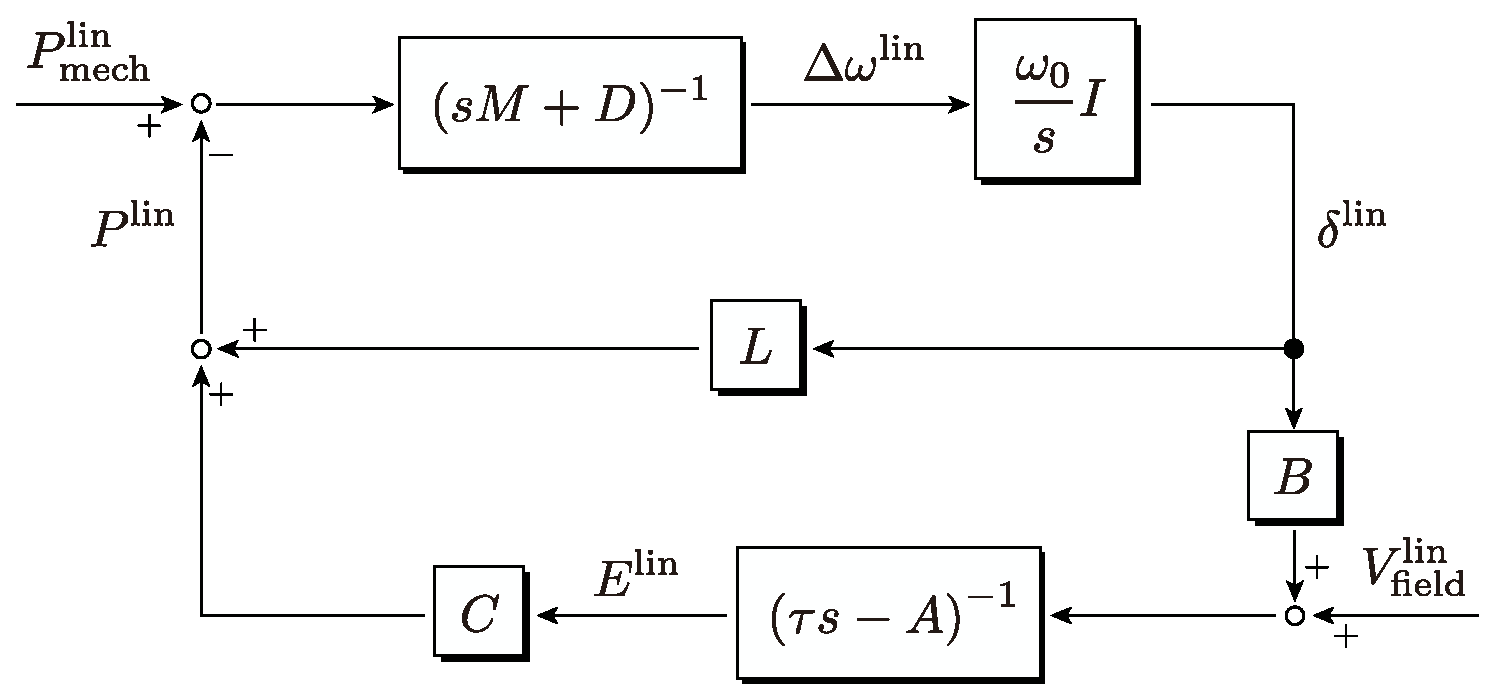
\includegraphics[width = .8\linewidth]{figs/blocklinsys3}
  \medskip
  \caption{\textbf{Block Diagram of Approximate Linear Model}}
  \label{fig:blocklinsys}
  \medskip
\end{figure}

\subsection{Stability analysis of approximate linear models}


\smallskip
\subsubsection{Stability of approximate linear models}

In this section, we consider numerically analyzing the stability of the
approximate linear model. Whether the approximate linear model of Equation
\ref{eq:lindyn} is stable or not is characterized by whether the internal states
of the generator groups return to the steady state satisfying the simultaneous
equations of Equation \ref{eq:kronss} in the event of a small disturbance in the
power system, such as temporary minor fluctuations in mechanical input or
excitation input of the generators, impedance values of the loads, current or
voltage values of the transmission lines, etc., from the reference values at the
steady state. In power system engineering, stability against such small
fluctuations is called \textbf{small signal stability}.

It should be noted that the stability of the approximate linear model of
Equation \ref{eq:lindyn} depends on the selection of the steady-state values of
the internal states of the generator groups $(\delta^{\star}, E^{\star})$ and
the steady-state values of external inputs $(P_{{\rm mech}}^{\star},V_{{\rm
field}}^{\star})$. Furthermore, changes in the admittance of the transmission
lines or the impedance of the loads alter the reduced conductance $G^{\rm
red}{ij}$ and reduced susceptance $B^{\rm red}{ij}$ of Equation \ref{eq:defkh}.
Therefore, the stability of the approximate linear model varies depending on
various model parameters mentioned above. The purpose of this section is to
numerically examine the relationship between the changes in these model
parameters and the stability of the approximate linear model.

\smallskip
\subsubsection{Stability analysis based on eigenvalues of the system matrix}

For the approximate linear model in Equation \ref{eq:lindyn}, if we
appropriately choose the steady-state values $(\delta^{\star},E^{\star})$ of the
internal states as parameters, then the system matrix $(L,A,B,C)$ in Equation
\ref{eq:sysmats} and the steady-state values $(P_{{\rm mech}}^{\star},V_{{\rm
field}}^{\star})$ of the external inputs satisfying Equation \ref{eq:kronss} are
determined dependently. Here, we consider setting

\[
  P_{{\rm mech}i}(t)=P_{{\rm mech}i}^{\star},\qquad
  V_{{\rm field}i}(t)
  =
  V_{{\rm field}i}^{\star},\qquad 
  \forall t\geq 0
\]
for all $i \in \mathcal{I}{\rm G}$ in the nonlinear differential equation system
model in Equation \ref{eq:krondyn}. We then assess the stability of the system
using the eigenvalues of the system matrix.

This means that in the approximate linear model of Equation \ref{eq:lindyn} the
following values are set:

\[
  P_{{\rm mech}}^{\rm lin}(t)
  =0,\qquad
  V_{{\rm field}}^{\rm lin}(t)
  =0
  ,\qquad 
  \forall t\geq 0
\]

In the following, under this assumption, we analyze the stability of an
autonomous approximate linear model with input set identically to zero, given
by:

\begin{equation}\label{eq:lindynu0}
  \mat{
    \dot{\delta}^{\rm lin} \\
    \Delta \dot{\omega}^{\rm lin} \\
    \dot{E}^{\rm lin}
  }
  =
  \underbrace{
    \mat{
      0 & \omega_0 I & 0\\
      -M^{-1}L & -M^{-1}D & -M^{-1}C \\
      \taud^{-1} B & 0 & \taud^{-1} A
    }
  }_{\Psi}
  \mat{
    \delta^{\rm lin} \\
    \Delta \omega^{\rm lin} \\
    E^{\rm lin}
  }
\end{equation}

Specifically, by examining the sign of the real part of the eigenvalues of the
matrix $\Psi$, we can determine the stability of this approximate linear model.
However, it should be noted that $\Psi$ generally has at least one zero
eigenvalue. In fact, from the structure of the matrices $L$ and $B$ in equation
\ref{eq:sysmats}, we have:

\begin{equation}\label{eq:LBker}
  L  \mathds{1} = 0
  ,\qquad
  B  \mathds{1} =0
\end{equation}

Therefore, for any model parameters, we have:

\[
  \Psi v=0 ,\qquad
  v:=\mat{
    \mathds{1} \\
    0 \\
    0
  }
\]

This means that $v$ is an eigenvector of $\Psi$ corresponding to a zero
eigenvalue. If the real parts of all eigenvalues, except for the zero
eigenvalue, are negative, then for any initial value, the solution trajectory of
Equation \ref{eq:lindynu0} satisfies:

\begin{equation}\label{eq:linmconv}
  \lim_{t\rightarrow \infty}\delta^{\rm lin}(t)= c_0  \mathds{1},\qquad
  \lim_{t\rightarrow \infty}\Delta \omega^{\rm lin}(t)=0 ,\qquad
  \lim_{t\rightarrow \infty} E^{\rm lin}(t)=0
\end{equation}

Here, $c_0$ is a constant determined by the initial value. Note that the value
of $c_0$ does not make a significant difference in the analytical results. This
is because in the differential equation system model of Equation
\ref{eq:krondyn_}, the rotor angle $\delta_i$ of a generator has meaning only in
relation to the difference between the rotor angle $\delta_j$ of other
generators. Specifically, if $(\delta^{\star},E^{\star})$ satisfies the system
of equations in equation \ref{eq:kronss} for a certain $(P_{{\rm
mech}}^{\star},V_{{\rm field}}^{\star})$, then $(\delta^{\star}+c_0
\mathds{1},E^{\star})$ also satisfies the same system of equations. Therefore,
$\delta^{\star}$ and $\delta^{\star}+c_0 \mathds{1}$ are essentially equivalent
steady-state values where all generator rotor angles are rotated by the same
amount of $c_0$. Equation \ref{eq:linmconv} means the asymptotic convergence of
solution trajectories to these essentially equivalent steady-state values.

\section{stability analysis of approximate linear models using numerical
calculations}\label{sec:numlinsta}

\subsection{Implementation of approximate linearization using a group of
partitioned modules}

In this section, we explain the implementation method for obtaining an
approximate linear model numerically. Specifically, we describe how to add the
functionality of linearization to the program that has been segmented into
module groups as explained in Sections \ref{sec:powfcal} and
\ref{sec:timerescal}.

In the numerical simulation program of the power system created in Section
\ref{sec:timerescal}, the following state and output equations are implemented
for each device as differential and algebraic equations, respectively:

\[
  \dot{x}_i = f_i^{(1)}(x_i, \bm V_i, \bm I_i, u_i)
  ,\qquad
  0 = f_i^{(2)} (x_i, \bm V_i, \bm I_i, u_i)
\]

In the following, we derive the approximate linear model in the vicinity of the
equilibrium point $(x_i^\star, \bm V_i^\star, \bm I_i^\star, u_i^\star)$ for the
device of interest. Specifically, we explain the implementation method of the
linear approximation function to the program that has been partitioned into the
module group described in Sections \ref{sec:powfcal} and \ref{sec:timerescal}.

For the numerical simulation program of the power system created in Section
\ref{sec:timerescal}, differential equations for the state and algebraic
equations for the output are implemented for each device as:

\[
  \dot{x}_i = f_i^{(1)}(x_i, \bm V_i, \bm I_i, u_i)
  ,\qquad
  0 = f_i^{(2)} (x_i, \bm V_i, \bm I_i, u_i)
\]

We consider the linearization of the functions $f_i^{(1)}$ and $f_i^{(2)}$ as
follows:

\begin{align}
  \hspace{-1mm}  f_i^{(1)} (x_i, \bm V_i, \bm I_i,u_i) &\approx A_i (x_i-x_i^\star) + B_{u_i}u_i\notag\\
    &+ B_{\bm{V}_i} \! \mat{
      \real[\bm V_i-\bm V^\star]\\ \imag[\bm V_i-\bm V^\star]
    }
    + 
    B_{\bm{I}_i} \! \mat{
      \real[\bm I_i-\bm I_i^\star]\\\imag[\bm I_i-\bm I_i^\star]
    }\label{eq:f_lin}\\
  \hspace{-1mm} f_i^{(2)} (x_i, \bm V_i, \bm I_i,u_i) &\approx C_i (x_i-x_i^\star) + D_{u_i}u_i\notag\\
    &+ 
    D_{\bm{V}_i}  \! \mat{
      \real[\bm V_i-\bm V^\star]\\ \imag[\bm V_i-\bm V^\star]
    }
    + D_{\bm{I}_i}  \! \mat{
      \real[\bm I_i-\bm I_i^\star]\\\imag[\bm I_i-\bm I_i^\star]\label{eq:g_lin}
    }
\end{align}

A system of simultaneous equations for each machine and algebraic equations for
the entire power system can be used to obtain an expression using ordinary
differential equations for the approximate linear model by eliminating all $\bm
V_i -\bm V^\star_i$ and $\bm I_i-\bm I_i^\star$, where $i \in {1,\ldots,N}$, as
follows:

\[
  \bm I_i - \bm I_i^\star = \sum_{j=1}^N \bm Y_{ij} (\bm{V}_j -\bm V^\star_j )
  ,\qquad
  i \in \{1,\ldots,N\}
\]

Here, $\bm{Y}_{ij}$ represents the $(i,j)$th element of the admittance matrix
$\bm{Y}$. Let us check the specific implementation method with the following
example.

\begin{example}[Implementation of Approximate Linear Model]

Equations \ref{eq:f_lin} and \ref{eq:g_lin} depend on the dynamic
characteristics of the device, so it is natural to implement the calculation of
coefficient matrices such as $A_i$ and $B_{u_i}$ in the classes of devices such
as generators and loads in the implementation example of Section
\ref{sec:powfcal}. For example, in the generator model:

\begin{flalign*}
  &\quad
  A_i = \mat{
  0 & \omega_0 & 0\\
  0 & -\tfrac{D_i}{M_i} & 0\\
  - \tfrac{1}{\tau_i}( \tfrac{X_i}{X_i'}-1)|\bm V_i^\star|\sfsin(\delta_i^\star-\angle\bm V_i^\star) &
  0& - \tfrac{X_i}{\tau_i X'_i}
  }
  &
  \end{flalign*}
  \begin{flalign*}
  &\quad
  B_{u_i} = \mat{
    0 \\ \tfrac{1}{M_i} \\ 0
  }
  ,\qquad
  B_{\bm{V}_i} = \mat{
    0 & 0\\ - \tfrac{\real [ \bm{I}_i^\star] }{M_i}  & - \tfrac{\imag[ \bm{I}_i^\star] }{M_i}\\
  \tfrac{1}{\tau_i}( \tfrac{X_i}{X_i'}-1) \sfcos \delta_i^\star& \tfrac{1}{\tau_i}( \tfrac{X_i}{X_i'}-1) \sfsin\delta_i^\star
  }
  &
\end{flalign*}
\begin{flalign*}
  &\quad
  B_{\bm{I}_i} = \mat{
    0 & 0\\ -\tfrac{\real [ \bm{V}_i^\star] }{M_i} & -\tfrac{\imag [ \bm{V}_i^\star] }{M_i}\\
  0 & 0 
  }
  ,\qquad
  C_i = \mat{
  E_i^\star\sfcos\delta^\star_i & 0 & \sfsin(\delta_i^\star)\\
  E_i^\star\sfsin\delta^\star_i & 0 & -\sfcos(\delta_i^\star)\\
  }
  &
\end{flalign*}
\begin{flalign*}
  &\quad
  D_{u_i} = \mat{0 \\ 0}
  ,\qquad
  D_{\bm{V}_i} = \mat{
    0 & -1\\ 1 & 0
  }
  ,\qquad
  D_{\bm{I}_i} =  \begin{bmatrix}
    -X_i' & 0\\0 & -X_i'
  \end{bmatrix}
  &
\end{flalign*}

If the calculation of these coefficient matrices is added to the
\verb|generator| class as a method named \verb|get_linear_matrix|, the program
\ref{program:generator_matrix} is obtained.

\smallskip
\begin{lstlisting}[language=Matlab, caption=generator.m, label={program:generator_matrix}]
classdef generator < handle
  
  properties
(Same as lines 4-11 in program 3-23)
    x_equilibrium
    V_equilibrium
    I_equilibrium
  end
  
  methods

(Same as lines 7 through 21 in program 3-34)

    function x_equilibrium = set_equilibrium(obj, V, I, P, Q)

(Same as lines 10 through 23 of program 3-28)

      obj.x_equilibrium = x_equilibrium;
      obj.V_equilibrium = V;
      obj.I_equilibrium = I;
    end
    
    function [A, Bu, BV, BI, C, Du, DV, DI] =...
        get_linear_matrix(obj)
      
      X = obj.X;
      X_prime = obj.X_prime;
      D = obj.D;
      M = obj.M;
      tau = obj.tau;
      
      omega0 = obj.omega0;
      delta = obj.x_equilibrium(1);
      E = obj.x_equilibrium(3);
      V = obj.V_equilibrium;
      Vabs = abs(obj.V_equilibrium);
      Vangle = angle(obj.V_equilibrium);
      I = obj.I_equilibrium;
      A = [0, omega0, 0;
        0, -D/M, 0;
        -(X/X_prime-1)*Vabs*sin(delta-Vangle)/tau,...
        0, -X/X_prime/tau];
      Bu = [0; 1/M; 0];
      BV = [0, 0;
        -real(I)/M, -imag(I)/M;
        (X/X_prime-1)*cos(delta)/tau,...
        (X/X_prime-1)*sin(delta)/tau];
      BI = [0, 0;
        -real(V)/M, -imag(V)/M;
        0, 0];
      C = [E*cos(delta), 0, sin(delta);
        E*sin(delta), 0, -cos(delta)];
      Du = [0; 0];
      DV = [0, -1; 1, 0];
      DI = -X_prime*eye(2);
    end

  end

end
\end{lstlisting}

In Program \ref{program:generator_matrix}, lines 18 to 20 in
\verb|set_equilibrium| store information about the equilibrium point used in the
calculation of the approximate linear model.

If implemented similarly for the constant impedance load model, the program
\ref{program:load_matrix} is obtained.

\smallskip
\begin{lstlisting}[language=Matlab, caption=load\_impedance.m, label={program:load_matrix}]
classdef load_impedance < handle
  
  properties
    z
    I_equilibrium
  end
  
  methods

(Same as lines 7 through 18 in program 3-35)
   
    function x_equilibrium = set_equilibrium(obj, V, I, P, Q)
      x_equilibrium = [];
      obj.z = -V/I;
      obj.I_equilibrium = I;
    end
    
    function [A, Bu, BV, BI, C, Du, DV, DI] =...
        get_linear_matrix(obj)
      
      A = [];
      Bu = zeros(0, 2);
      BV = zeros(0, 2);
      BI = zeros(0, 2);
      C = zeros(2, 0);
      I = obj.I_equilibrium;
      z = obj.z;
      Du = [real(z)*real(I), imag(z)*imag(I);
        real(z)*imag(I), imag(z)*real(I)];
      DV = eye(2);
      DI = [real(z), -imag(z); imag(z), real(z)];
    end
    
  end
  
end
\end{lstlisting}

By using the class of equipment such as modified generators and loads, the
function for obtaining an approximate linear model can be described as shown in
Program \ref{program:linearization}.

\smallskip
\begin{lstlisting}[language=Matlab, caption=get\_linear\_model.m, label={program:linearization}]
function sys = get_linear_model(a_component, Y)

  A = cell(numel(a_component), 1);
  Bu = cell(numel(a_component), 1);
  BV = cell(numel(a_component), 1);
  BI = cell(numel(a_component), 1);
  C = cell(numel(a_component), 1);
  Du = cell(numel(a_component), 1);
  DV = cell(numel(a_component), 1);
  DI = cell(numel(a_component), 1);

  for k = 1:numel(a_component)
    component = a_component{k};
    [A{k}, Bu{k}, BV{k}, BI{k}, C{k}, Du{k}, DV{k}, DI{k}] =...
      component.get_linear_matrix();
  end

  A = blkdiag(A{:});
  Bu = blkdiag(Bu{:});
  BV = blkdiag(BV{:});
  BI = blkdiag(BI{:});
  C = blkdiag(C{:});
  Du = blkdiag(Du{:});
  DV = blkdiag(DV{:});
  DI = blkdiag(DI{:});

  Ymat = zeros(size(Y, 1)*2, size(Y, 2)*2);
  Ymat(1:2:end, 1:2:end) = real(Y);
  Ymat(2:2:end, 1:2:end) = imag(Y);
  Ymat(1:2:end, 2:2:end) = -imag(Y);
  Ymat(2:2:end, 2:2:end) = real(Y);

  nx = size(A, 1);

  A11 = A;
  A12 = [BV, BI];
  A21 = [C; zeros(size(Ymat, 1), nx)];
  A22 = [DV, DI; Ymat, -eye(size(Ymat))];

  B1 = Bu;
  B2 = [Du; zeros(size(Ymat, 1), size(Du, 2))];


  Aout = A11 - A12/A22*A21;
  Bout = B1 - A12/A22*B2;
  Cout = eye(nx);
  Dout = 0;

  sys = ss(Aout, Bout, Cout, Dout);

end
\end{lstlisting}

In lines 12 to 16 of Program \ref{program:linearization}, the coefficient matrix
of the approximate linear model is obtained from each equipment. Additionally,
by eliminating the voltage and current phases of all buses from lines 27 to 47,
an expression for the approximate linear model's system of ordinary differential
equations is obtained.

The approximate linear model can be used as follows by using Program
\ref{program:linearization}.


\smallskip
\begin{lstlisting}[language=Matlab, caption=main\_linearization.m, label={program:main_linearization}]
(Same as lines 1 through 23 in Program 3-30)

sys = get_linear_model(a_component, Y);

sys = sys(2, 1);
nyquist(sys)
\end{lstlisting}

In this example, an approximate linear model is constructed in line 5 with the
mechanical input $P_{{\rm mech}1}$ of generator 1 as input and the frequency
deviation $\Delta\omega_1$ of generator 1 as output. In addition, a Nyquist plot
is drawn in line 6.
\end{example}

In the mathematical analysis of Section \ref{sec:linaproxt}, an approximate
linear model is derived from a nonlinear system of ordinary differential
equations where all buses are Kron reduced. On the other hand, in the numerical
implementation of this section, the nonlinear differential-algebraic equation
system is first linearized, and then Kron reduction is applied to construct the
ordinary differential equation system. It should be noted that this is because
in the power system model with Kron reduction, expressions generally involve a
mixture of information about equipment, buses, and transmission lines.

To increase the readability and expandability of the program, it is important to
modularize each element appropriately, as in the implementation of this section.

\subsection{Numerical analysis of small signal stability}

Let us perform a stability analysis based on approximate linearization for an
actual electrical power system model consisting of three generators.

%\begin{figure}[t]
%\centering
%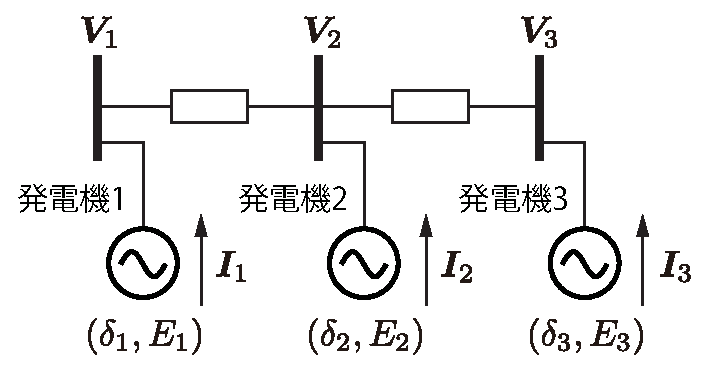
\includegraphics[width = .5\linewidth]{figs/gen3ex}
%\medskip
%\caption{\textbf{3つの発電機からなる電力系統モデル}}
%\label{fig:3genex}
%\medskip
%\end{figure}
%
%\begin{figure}[t]
%  \centering
%  {
%  \begin{minipage}{0.49\linewidth}
%    \centering
%    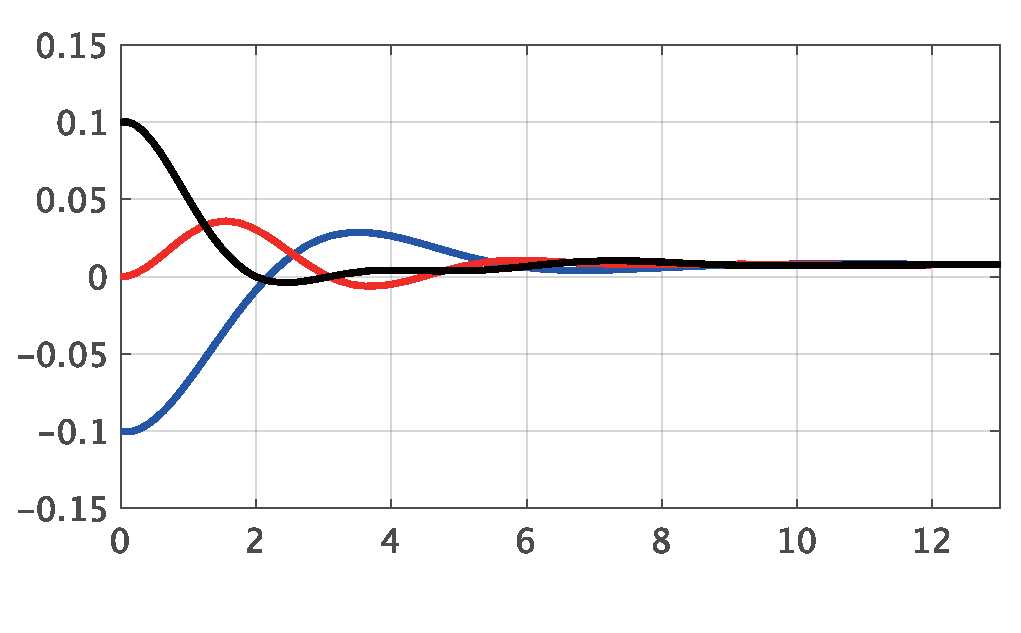
\includegraphics[width = 1.0\linewidth]{figs/delta}
%    \subcaption{ $\delta^{\rm lin}$ }
%    \medskip
%  \end{minipage}
%  \begin{minipage}{0.49\linewidth}
%    \centering
%    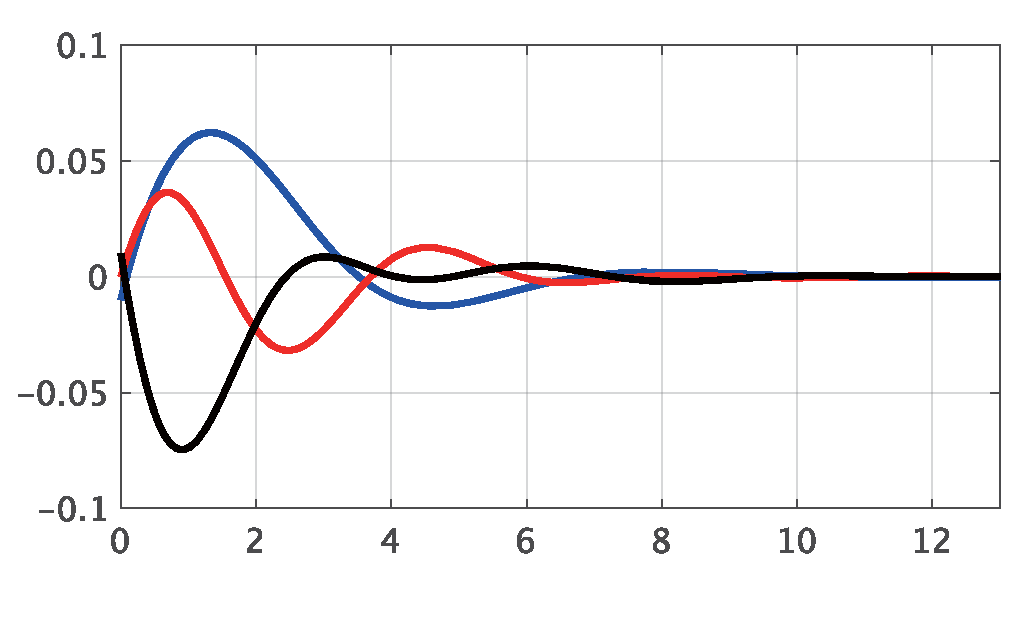
\includegraphics[width = 1.0\linewidth]{figs/omega}
%    \subcaption{ $\Delta \omega^{\rm lin}$ }
%    \medskip
%  \end{minipage}
%%  \begin{minipage}{0.32\linewidth}
%    \centering
%    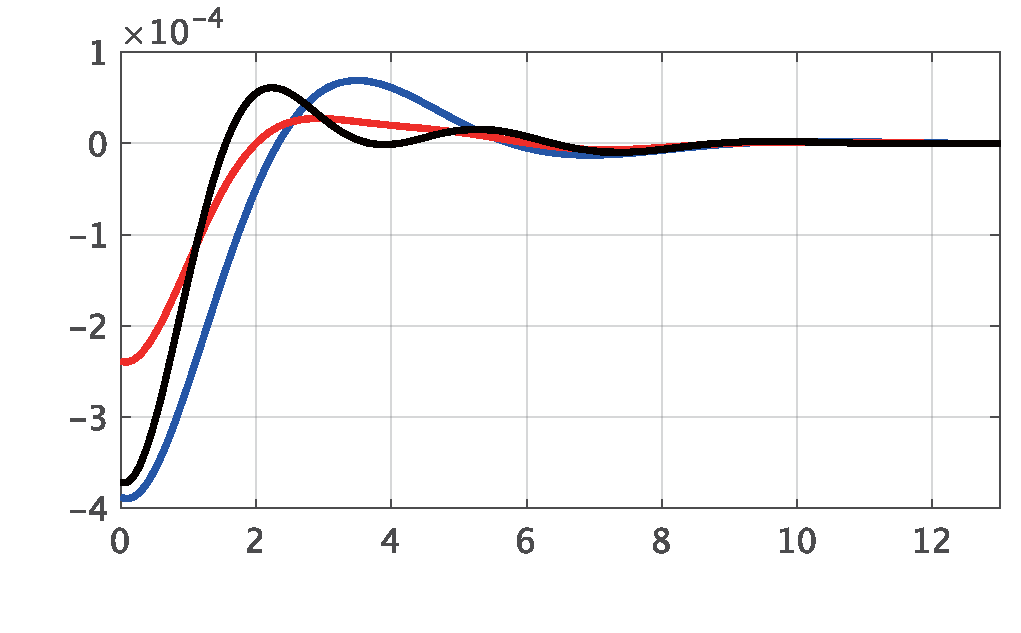
\includegraphics[width = .49\linewidth]{figs/E}
%    \subcaption{ $E^{\rm lin}$ }
%%  \end{minipage}
%  }
%  \medskip
%  \caption{\textbf{近似線形モデルの初期値応答}}
%  \label{fig:timeex}
%\medskip
%\end{figure}


\begin{figure}[t]
  \centering
  {
  \begin{minipage}{0.49\linewidth}
    \centering
    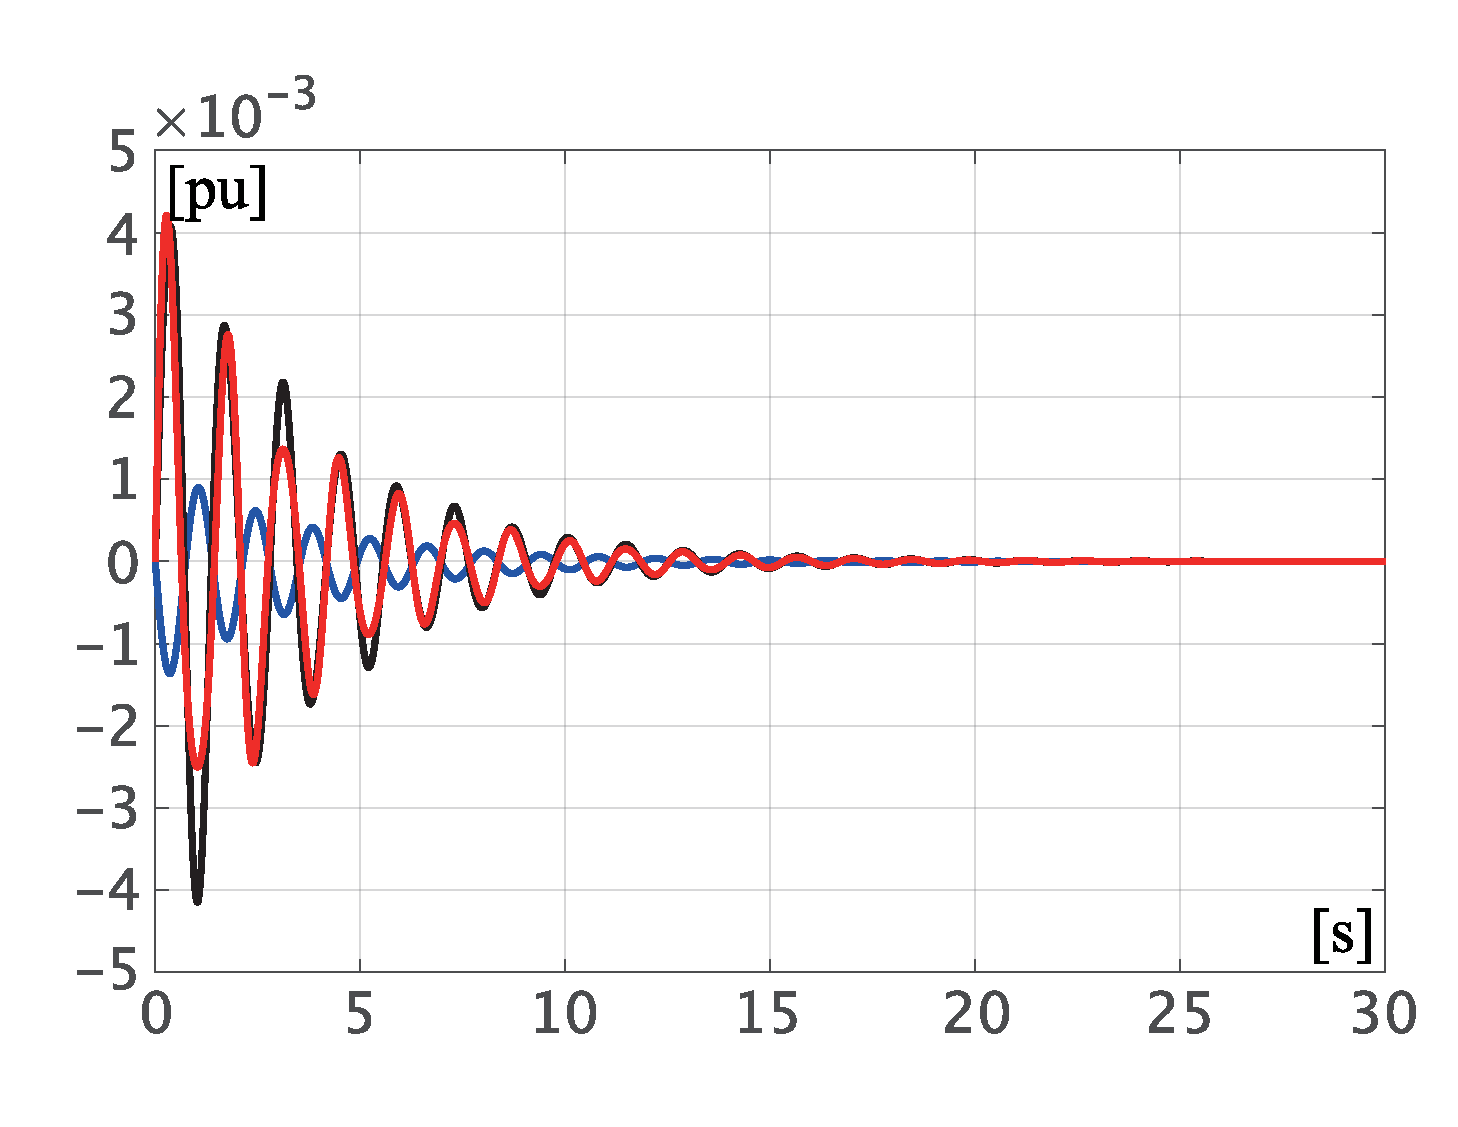
\includegraphics[width = 1.0\linewidth]{figs/Domegalin}
    \subcaption{ $\Delta \omega^{\rm lin}$ }
    \medskip
  \end{minipage}
  \begin{minipage}{0.49\linewidth}
    \centering
    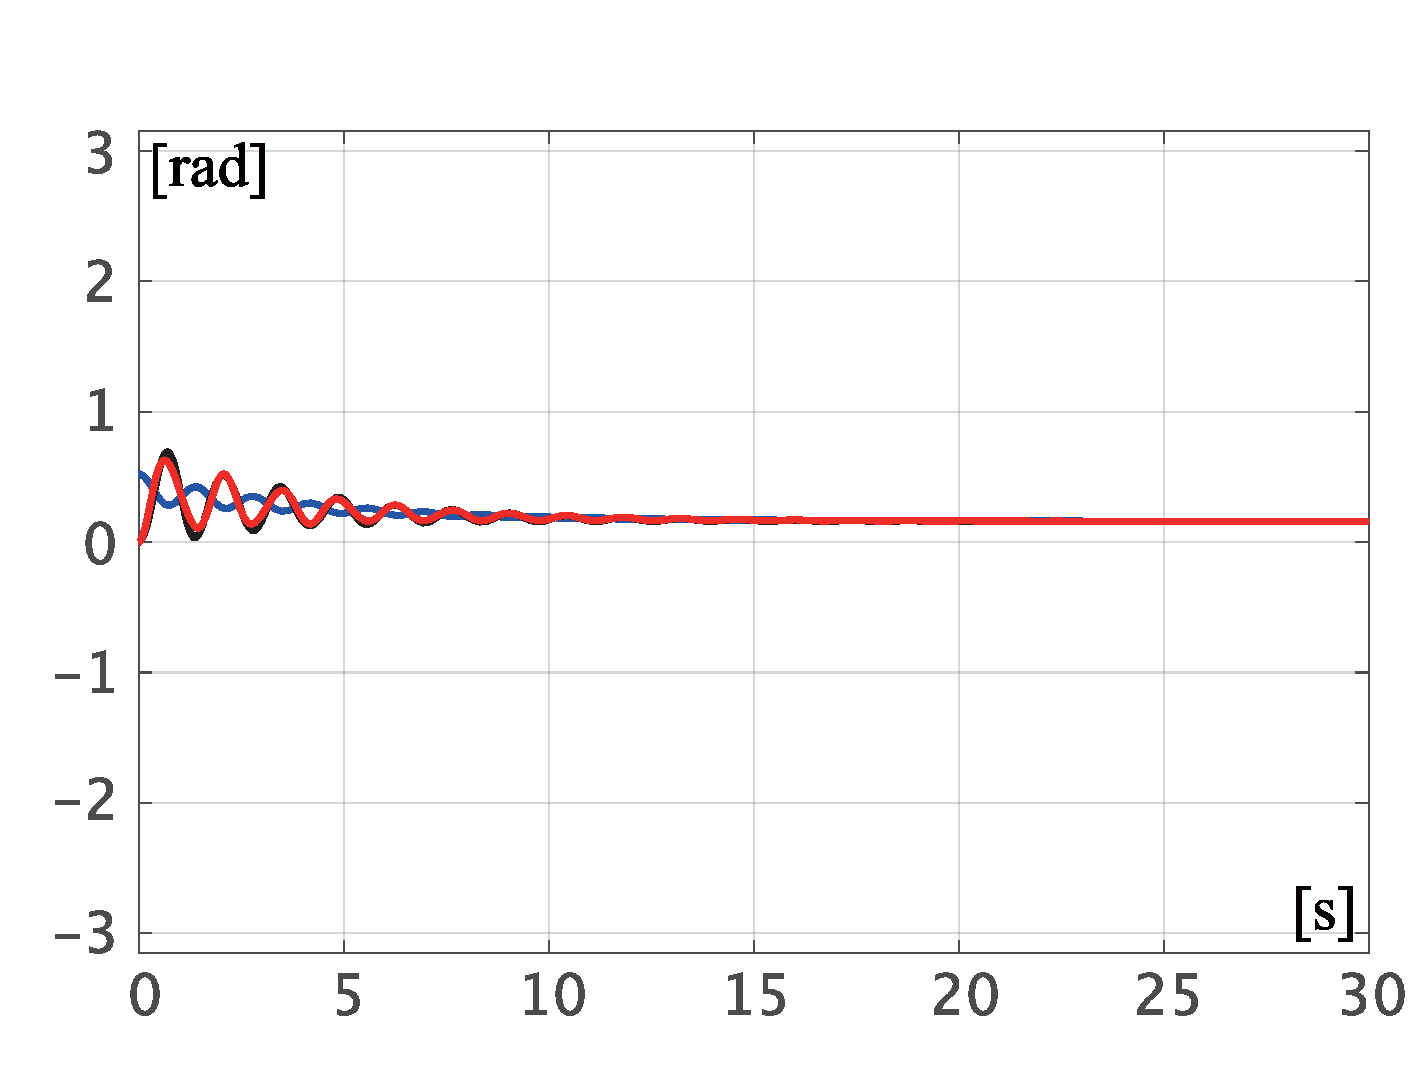
\includegraphics[width = 1.0\linewidth]{figs/deltalin}
    \subcaption{ $\delta^{\rm lin}$ }
    \medskip
  \end{minipage}
 \begin{minipage}{0.49\linewidth}
    \centering
    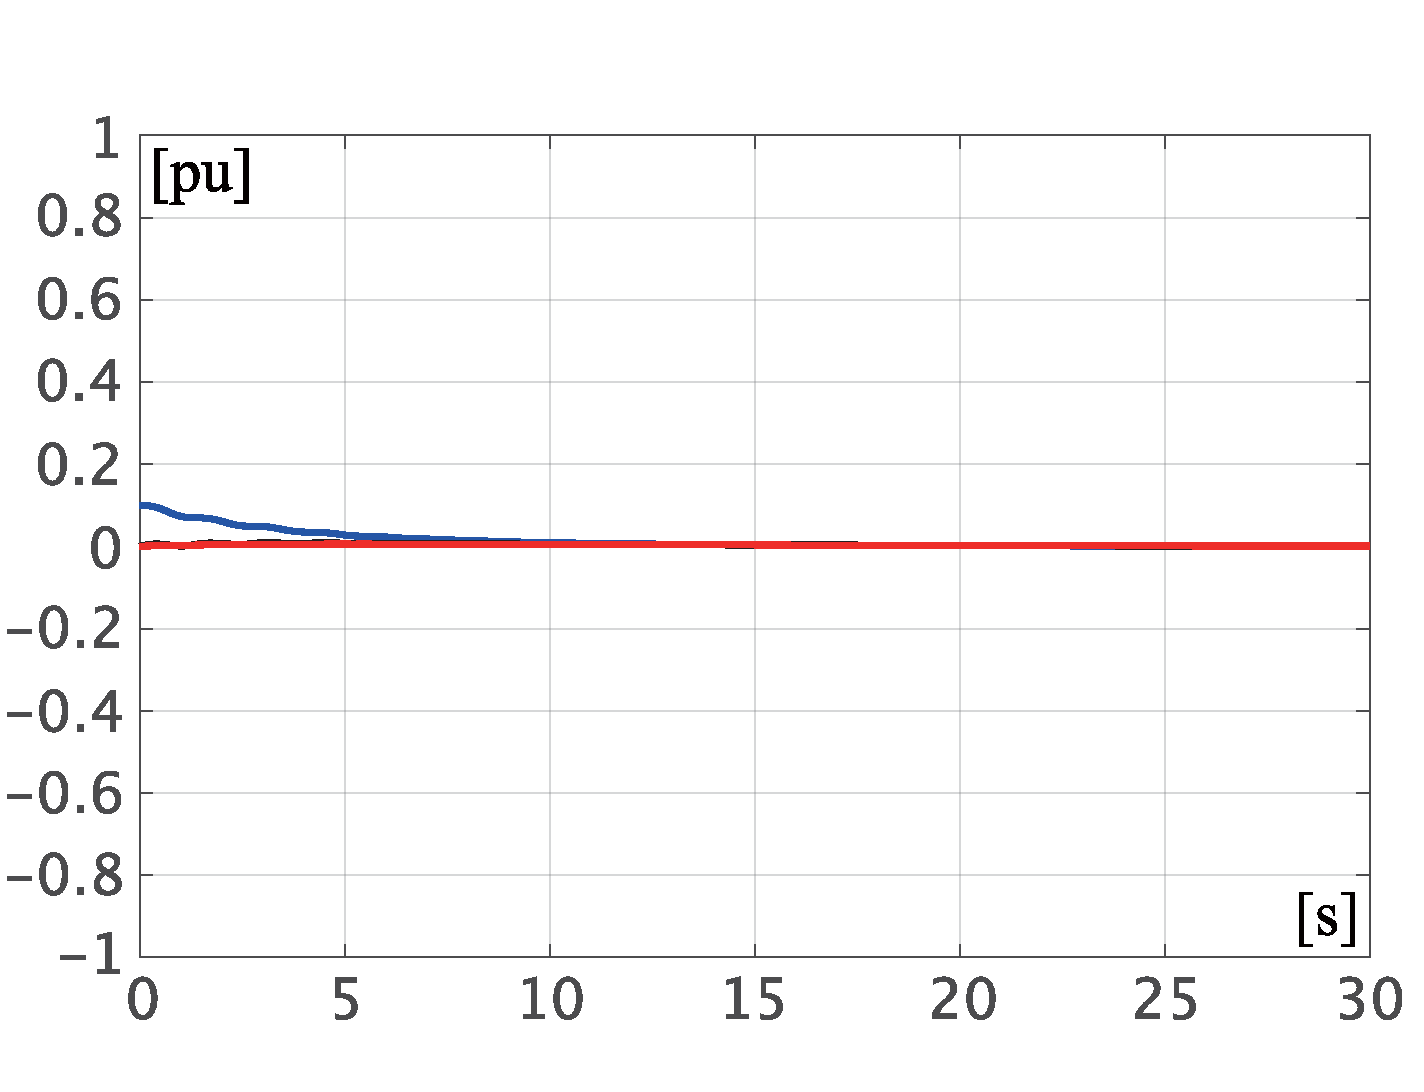
\includegraphics[width = 1.0\linewidth]{figs/Elin}
    \subcaption{ $E^{\rm lin}$  }
    \medskip
  \end{minipage}
  \begin{minipage}{0.49\linewidth}
    \centering
    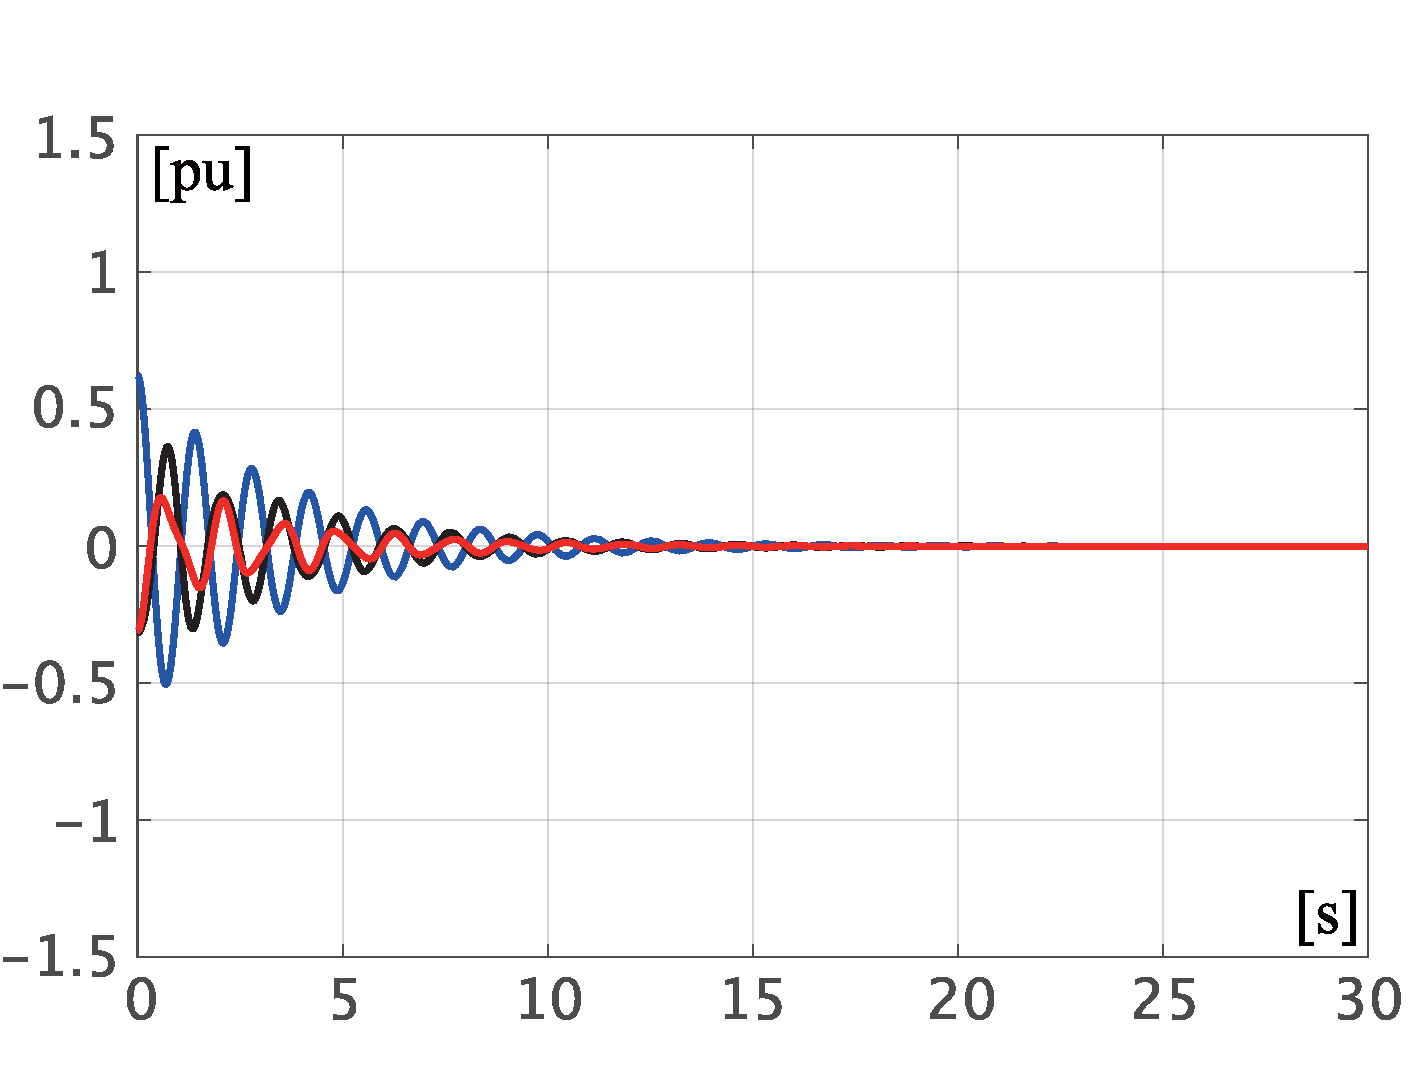
\includegraphics[width = 1.0\linewidth]{figs/Plin}
    \subcaption{ $P^{\rm lin}$ }
    \medskip
  \end{minipage}
  }
  \medskip
  \caption{\textbf{Initial value response of approximate linear model}
  \\  \centering(Blue: Generator 1, Black: Generator 2, Red: Generator 3)}
  \label{fig:timeex}
\medskip
\end{figure}


%\begin{figure}[t!]
%\centering
%  {
%    \centering
%    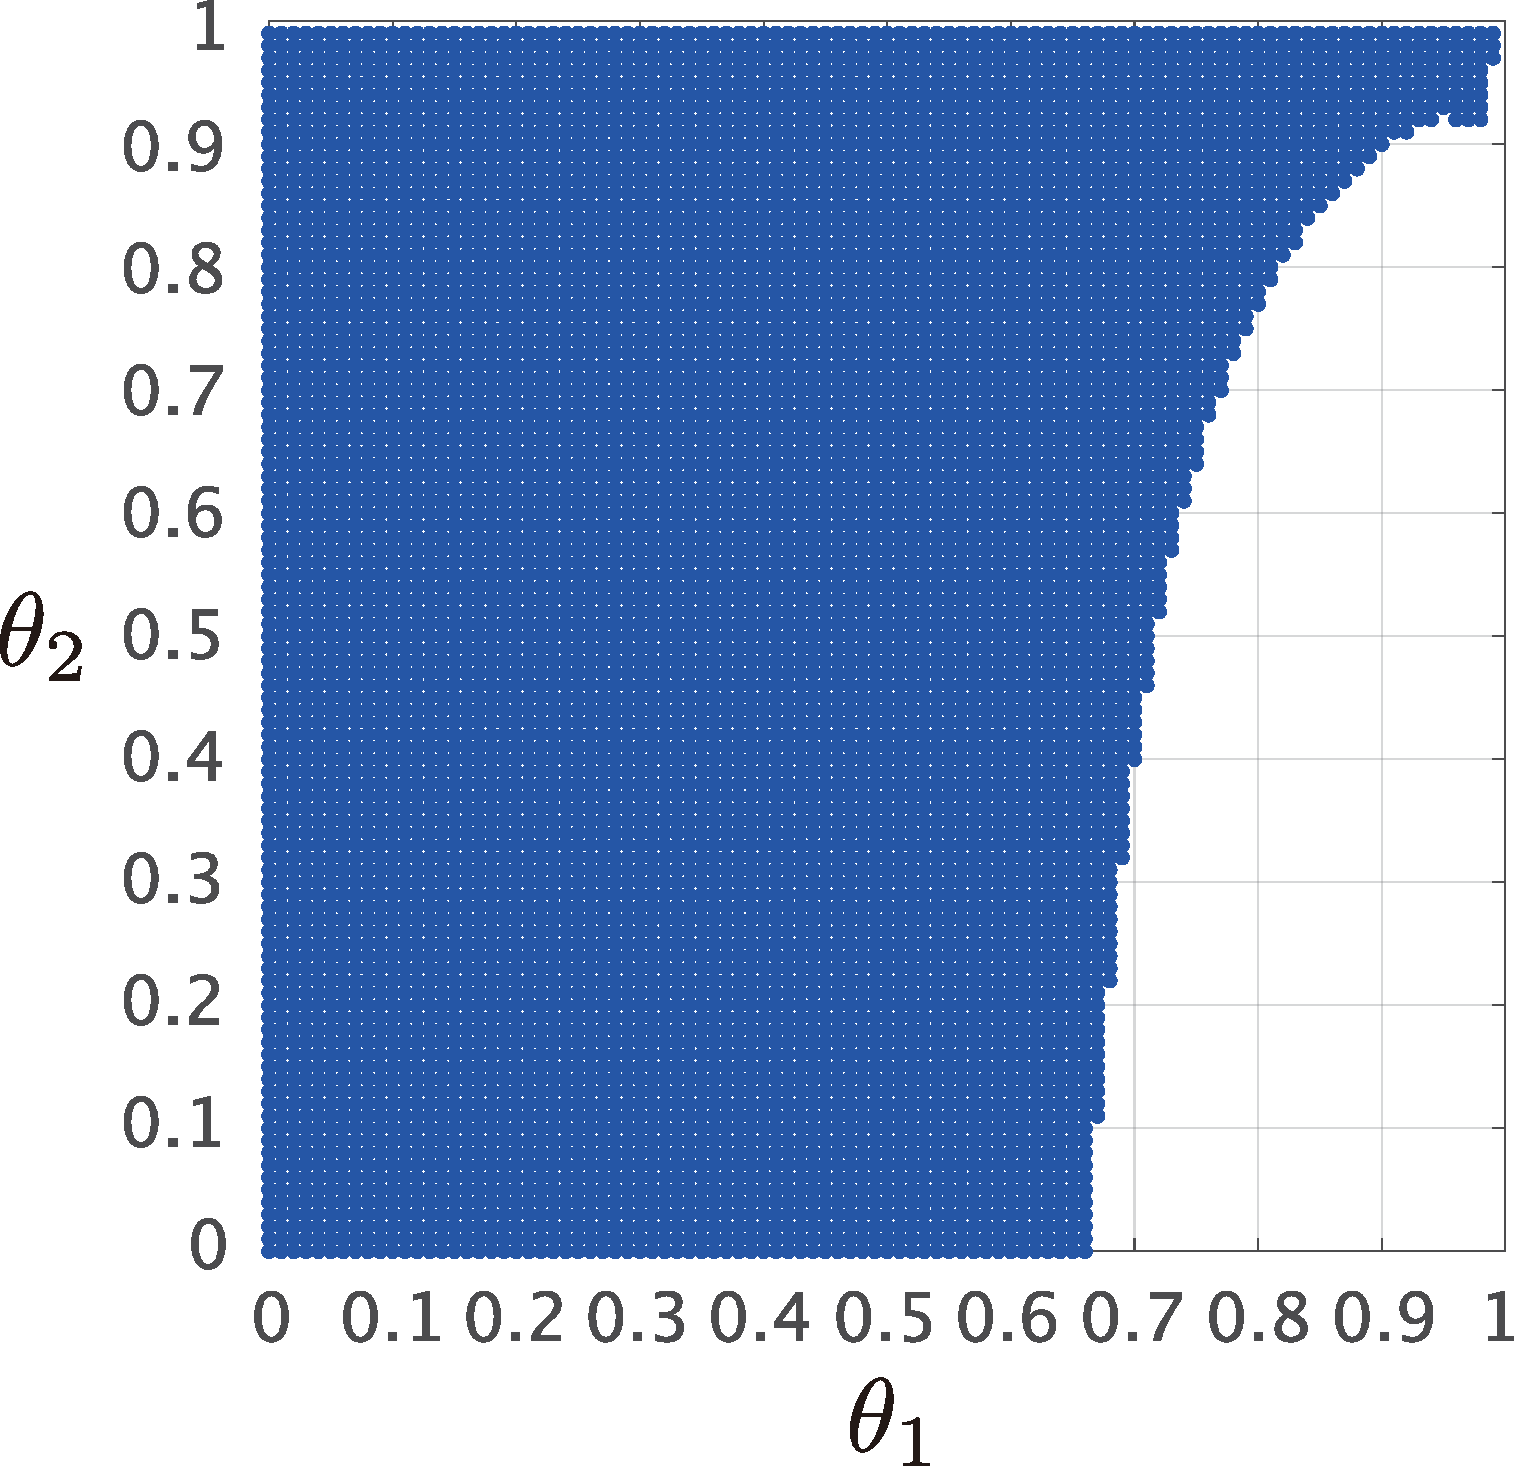
\includegraphics[width = .4\linewidth]{figs/gam01}
%    \subcaption{ $\gamma=0.1$ }
%    \centering
%    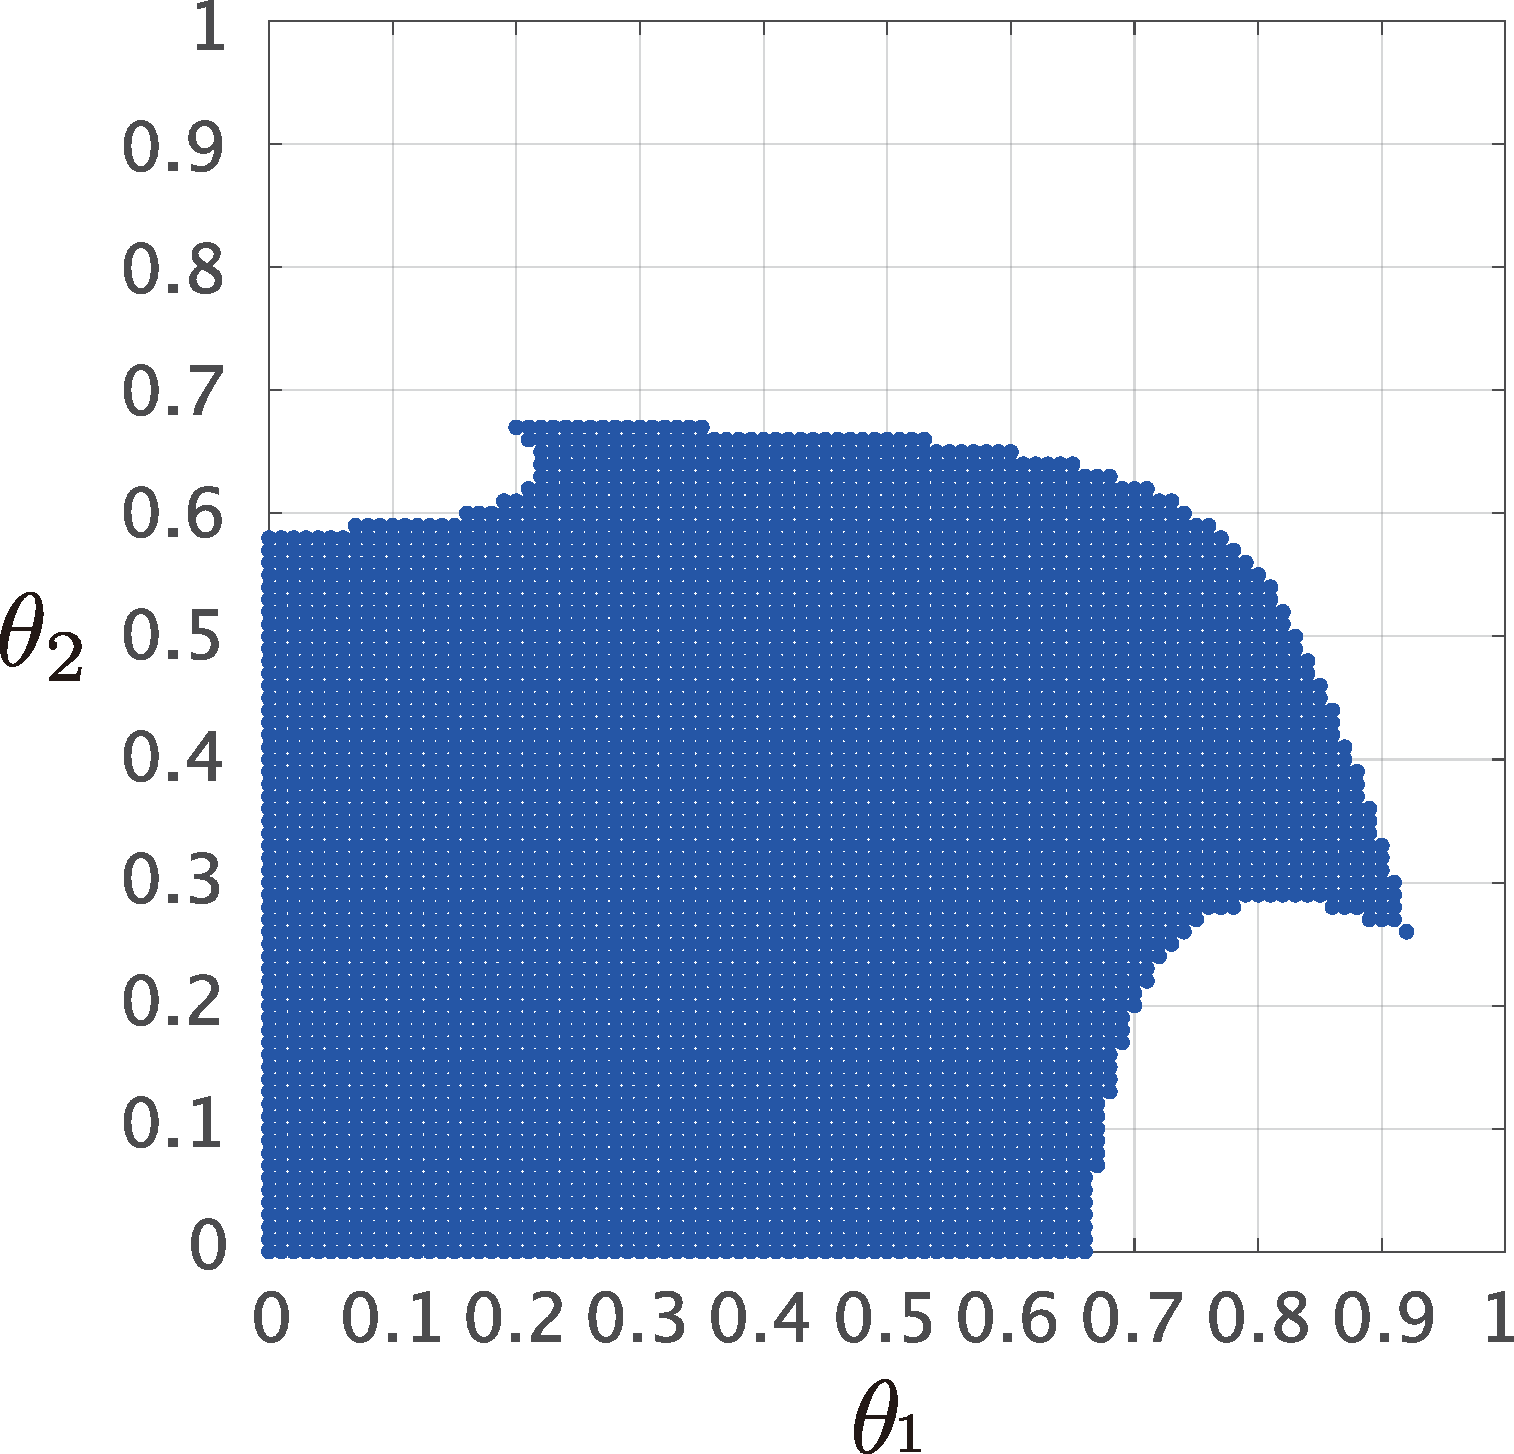
\includegraphics[width = .4\linewidth]{figs/gam2}
%    \subcaption{ $\gamma=2$ }
%    \centering
%    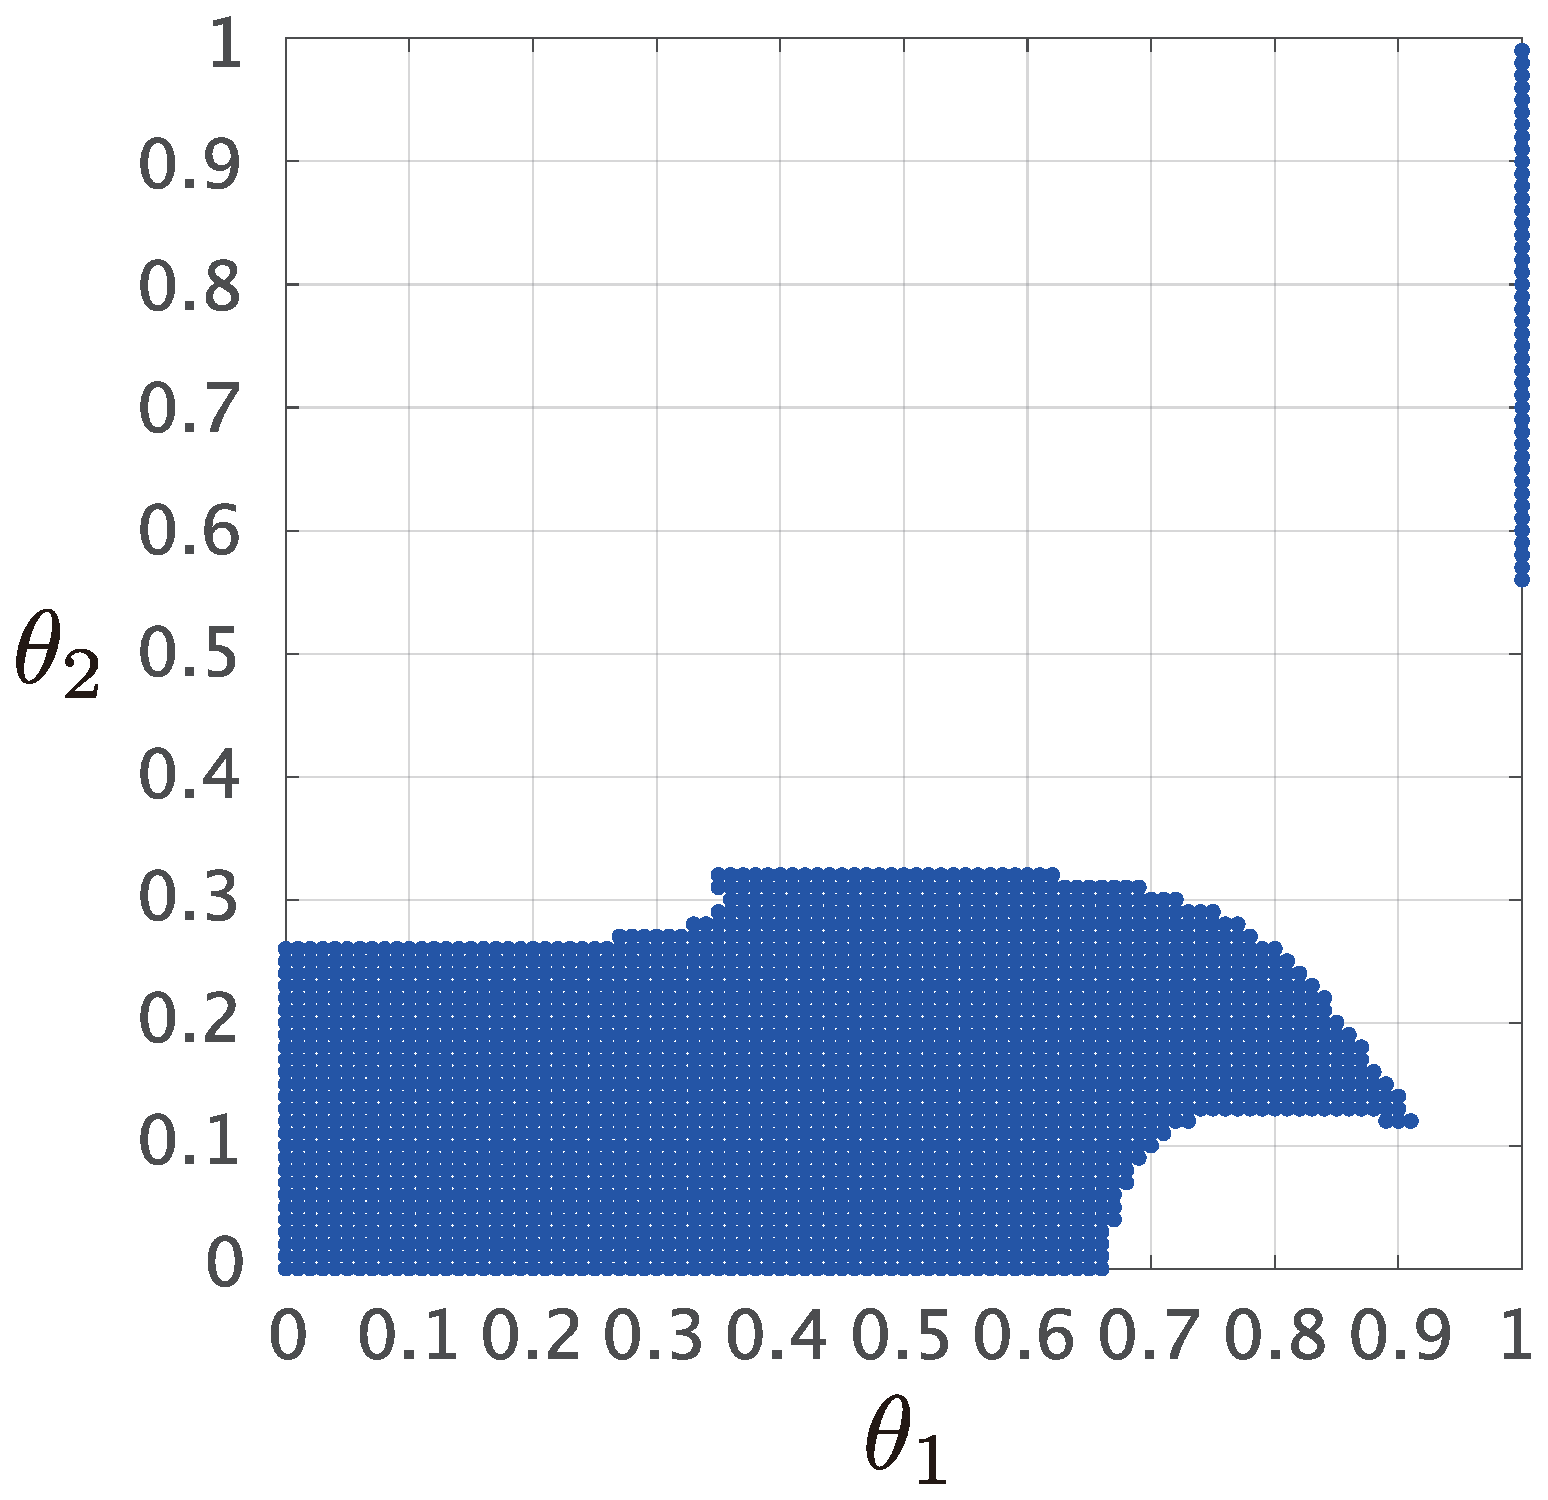
\includegraphics[width = .4\linewidth]{figs/gam5}
%    \subcaption{ $\gamma=5$ }
%  }
%\caption{近似線形モデルが安定となるパラメータの領域}
%\label{fig:gamsta}
%\medskip
%\end{figure}



\begin{example}{Numerical stability analysis of the linearized model}\label{ex:linsyssim}
Let us consider an electrical power system model consisting of three generators
discussed in the Example \ref{ex:Kronode}. The constant of the generators and
transmission lines are set to the same value as in the Example \ref{ex:Kronode},
and a linear approximation model for Equation \ref{eq:lindynu0} is derived with
the approximate of the steady value shown in \ref{table:gensteady}. Figure
\ref{fig:timeex} shows the time response When the initial values are set as
follows to correspond to Equation \ref{eq:exdelE0}:

\begin{equation}\label{eq:linmini}
  \delta^{\rm lin}(0)
  =
  \mat{
    \tfrac{\pi}{6} \\
    0 \\
    0
  },\quad
  \Delta \omega^{\rm lin}(0)
  =
  \mat{
    0 \\
    0 \\
    0
  },\quad
  E^{\rm lin}(0)
  =
  \mat{
    0.1 \\
    0 \\
    0
  }
\end{equation}

The blue, black, and red lines represent generators 1, 2, and 3, respectively.
From this figure, we can see that the internal state of the generator group
converges asymptotically as given in \eqref{eq:linmconv}.  Moreover, it
approximately reproduces the initial value response of the nonlinear model shown
in Fig. \ref{fig:Kron0}.

Next, we parameterize the constants and steady-state values of the generators
and transmission lines to analyze the stability of the resulting approximate
linear model. For the generator constants, we compare the cases where all the
damping coefficients are set to 10 and where they are set to 0.1, i.e., we
consider the two cases:

\[
  (D_1,D_2,D_3)= (10,10,10), \qquad
  (D_1,D_2,D_3)= \left(0.1,0.1,0.1\right)
\]

Other constants are set to the values in Table \ref{table:genparams}. In
addition, the steady-state values of the rotor angle differences are expressed
in terms of a parameter $\theta_1 \in [0, 1]$ as follows:

\begin{equation}
  \delta_{12}^{\star}= - \frac{\pi}{2} \theta_1
  ,\qquad
  \delta_{13}^{\star}=  \frac{\pi}{2} \theta_1
\end{equation}

Here, $\theta_1$ is a parameter that specifies the magnitude of the rotor angle
difference in the steady-state. By varying this value, the system matrix in
\ref{eq:sysmats} changes. Note that the steady-state values of the internal
voltages are not changed from the values in Table \ref{table:gensteady}.

The admittance matrix is also modified as follows. Using the admittance values
$\bm{y}_{12}$ and $\bm{y}_{23}$ in Equation \ref{eq:defadpara}, the admittance
matrix of the power system in Equation \ref{eq:exY} is constructed. The real
part of this admittance matrix, which is the conductance matrix, is denoted as
$G_0$, and the imaginary part, which is the susceptance matrix, is denoted as
$B_0$. Specifically,

\begin{equation}
  \begin{aligned}
    \spliteq{
    G_0 &=
    \mat{
    1.3652 &  -1.3652 &     0 \\
    -1.3652 &   3.3074 &  -1.9422 \\
    0 &  -1.9422 &  1.9422
    }, \\
    B_0 & =
    \mat{
    -11.6041  & 11.6041    &    0 \\
      11.6041 &  -22.1148  &  10.5107 \\
      0  &  10.5107 &  -10.5107
    }
    }
  \end{aligned}
\end{equation}

Using the parameter $\theta_2 \in [0,5]$, we express the reference admittance
matrix as follows:

\begin{equation}\label{eq:Y0theta2}
  \bm{Y}_0(\theta_2)
  :=
  \theta_2 G_0
  +
  \bm{j}  B_0
\end{equation}

Here, $\theta_2$ is a parameter that specifies the size of the real part
(conductance matrix). For comparison, we consider two parameterized admittance
matrices:

\begin{equation*}
  \bm{Y} = \bm{Y}_0(\theta_2)
  ,\qquad
  \bm{Y} = \tfrac{\bm{Y}_0(\theta_2)}{100}
\end{equation*}

The changes in the admittance matrix are approximately represented in the
linearized model by the changes in the values of the reduced conductor $B^{\rm
red}{ij}$ and the reduced susceptance $G^{\rm red}{ij}$ in equation
\ref{eq:defkh}. The parameter settings for the comparison are summarized in
Table \ref{table:parasetcom}.

Let us numerically analyze the stability of the approximate linear model by
varying the parameters $(\theta_1, \theta_2)$ for each case (a)-(d) in
\TABref{table:parasetcom}. Specifically, we will check whether the approximate
linear model is stable or not by examining the eigenvalues of $\Psi$ in Equation
\ref{eq:lindynu0} by varying $\theta_1$ and $\theta_2$ on a grid of 100
equidistant points each. The results are shown in \FIGref{fig:stacheck}. The
blue area represents the parameter region where the approximate linear model is
stable. First, in the case of (a), we see that the approximate linear model is
stable regardless of the size of the conductance matrix specified by $\theta_2$,
as long as $\theta_1$ is below approximately 0.4, which corresponds to a rotor
angle difference of approximately $36^\circ$ in the steady state. The same
result is obtained for case (b), where the generator's damping coefficient is
small at 0.1.

Next, we examine the results for cases (c) and (d), where the admittance matrix
is multiplied by $\tfrac{1}{100}$. In this case, we find that when $\theta_2$
is small and the size of the conductance matrix is around 1, the approximate
linear model is stable as long as the rotor angle difference in the steady state
is below approximately $76^\circ$. We also find that as $\theta_2$ increases to
2 or more, the upper limit of the rotor angle difference for stability of the
approximate linear model decreases.
\end{example}

\begin{table}[h]
\medskip
 \caption{\textbf{Parameter settings to compare}}
 \label{table:parasetcom}
 \centering
  \begin{tabular}{|c|c|c|c|c|c|c|}
   \hline
 &    $D=(10,10,10)$ &   $D=(0.1,0.1,0.1)$ \\
   \hline 
 $\bm{Y} =\bm{Y}_0$ & (a) & (b) \\
   \hline
 $\bm{Y} = \bm{Y}_0/100  $  & (c) & (d) \\
   \hline
  \end{tabular}
\end{table}

\begin{figure}[t!]
  \centering
  {
  \begin{minipage}{0.49\linewidth}
    \centering
    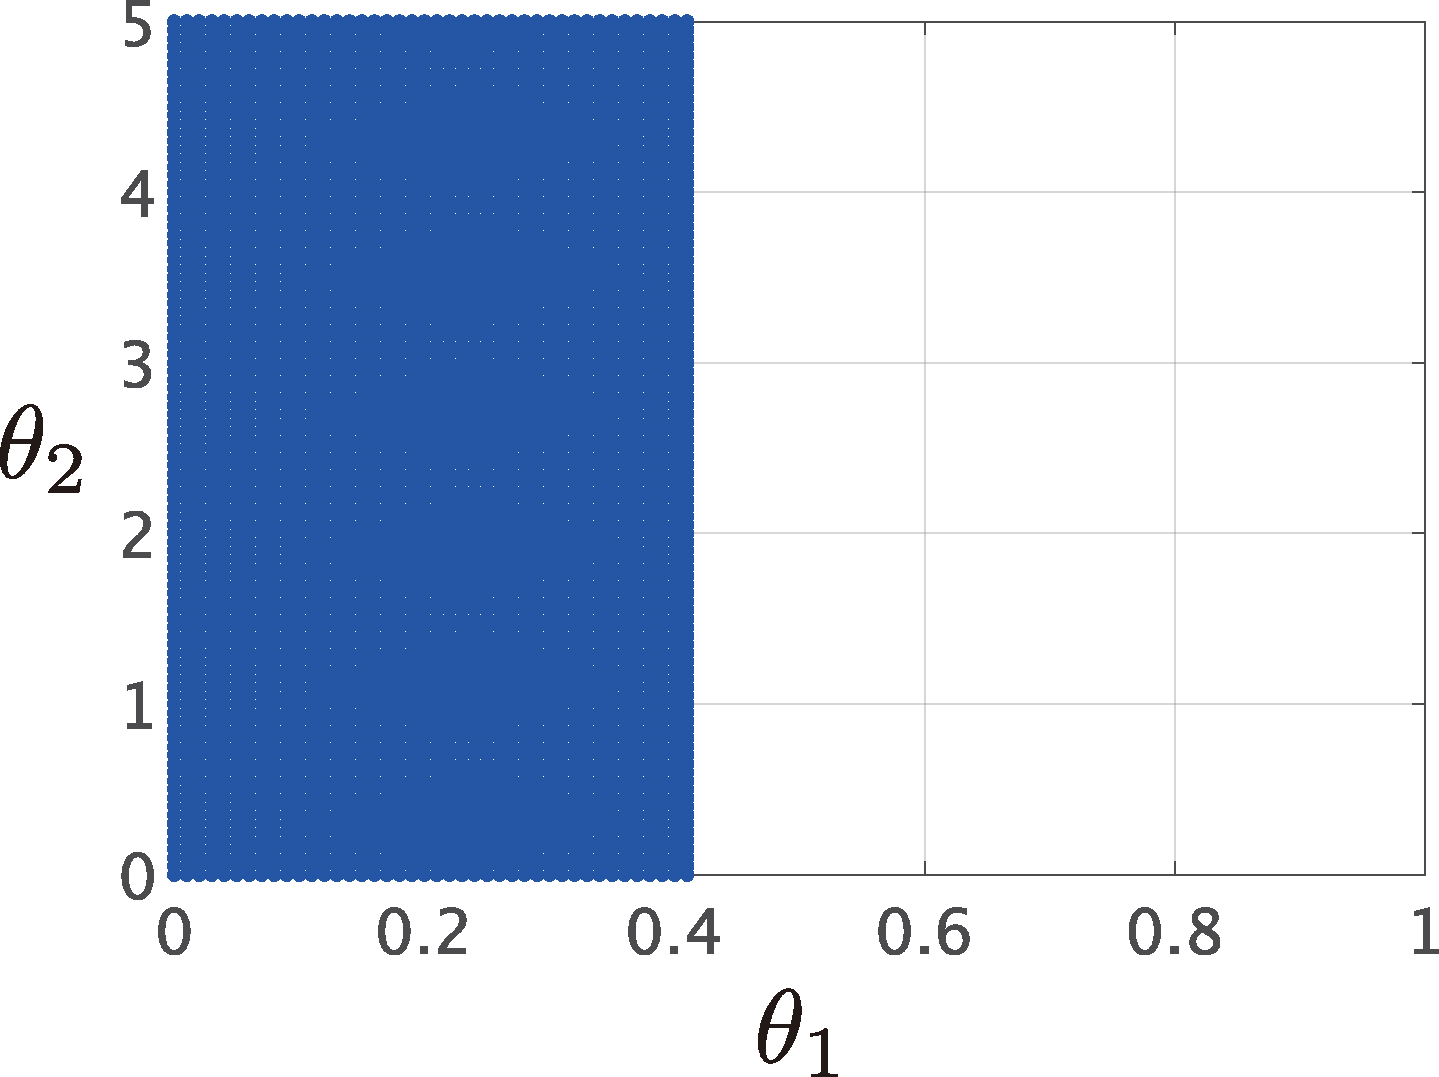
\includegraphics[width = 0.90\linewidth]{figs/Y1D1}
    \subcaption{ $D=(10,10,10)$,$\bm{Y}=\bm{Y}_0$ }
    \medskip
  \end{minipage}
  \begin{minipage}{0.49\linewidth}
    \centering
    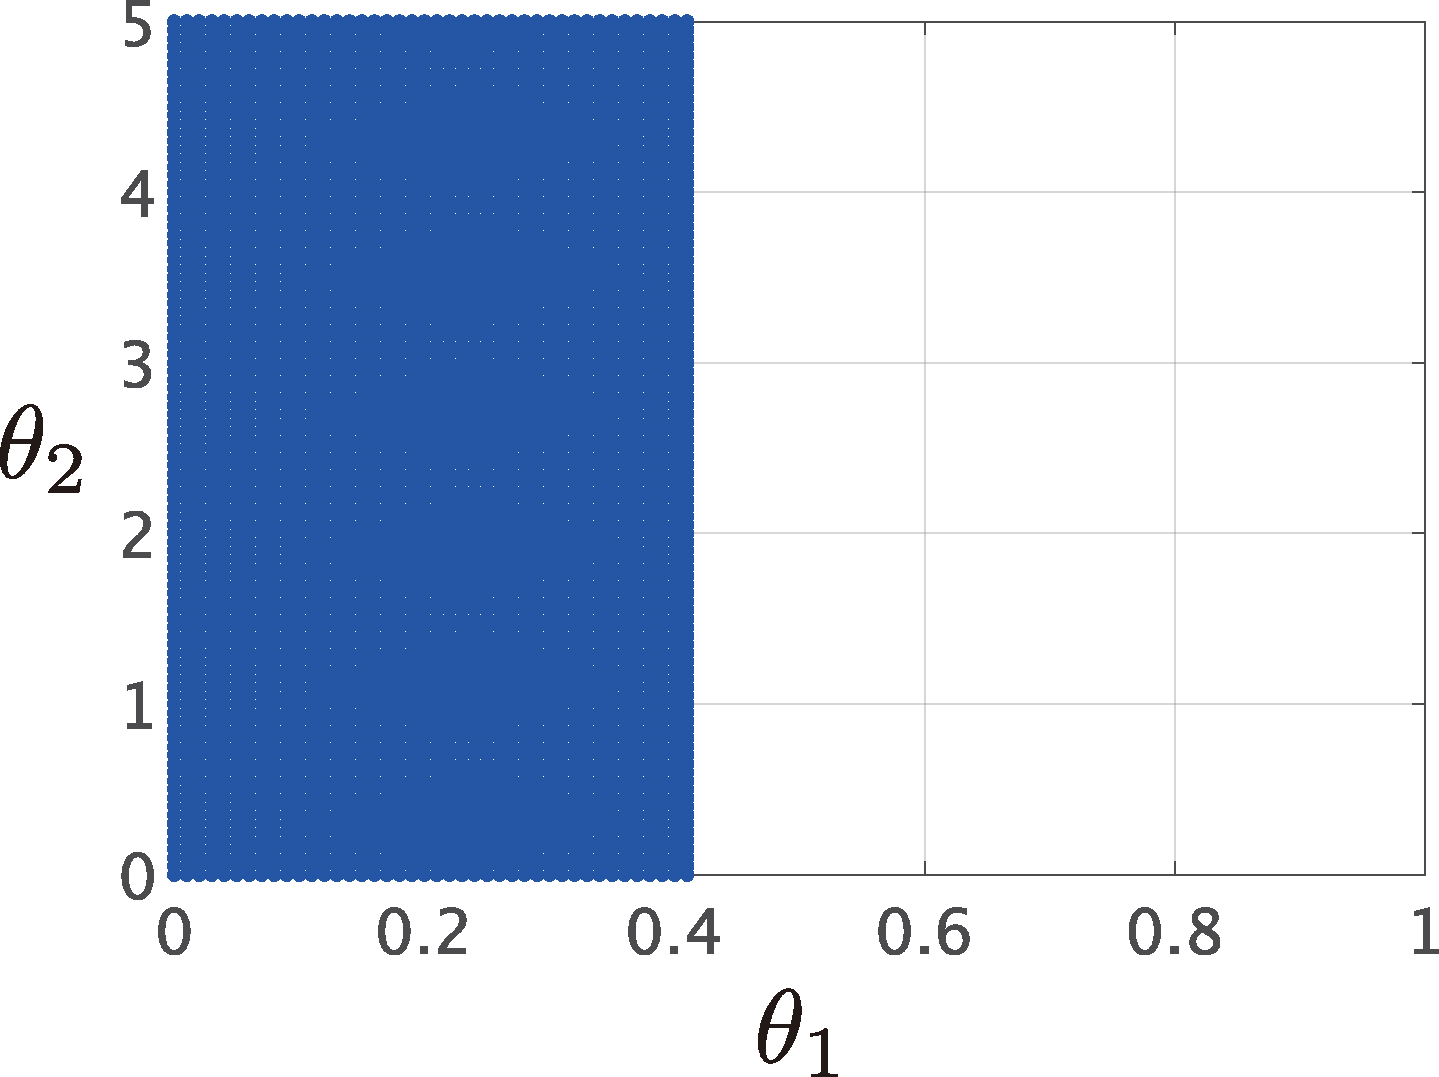
\includegraphics[width = 0.90\linewidth]{figs/Y1D0.01}
    \subcaption{$D=(\tfrac{1}{10}\tfrac{1}{10},\tfrac{1}{10})$,$\bm{Y}=\bm{Y}_0$ }
    \medskip
  \end{minipage}
}
  \centering
  {
  \begin{minipage}{0.49\linewidth}
      \centering
    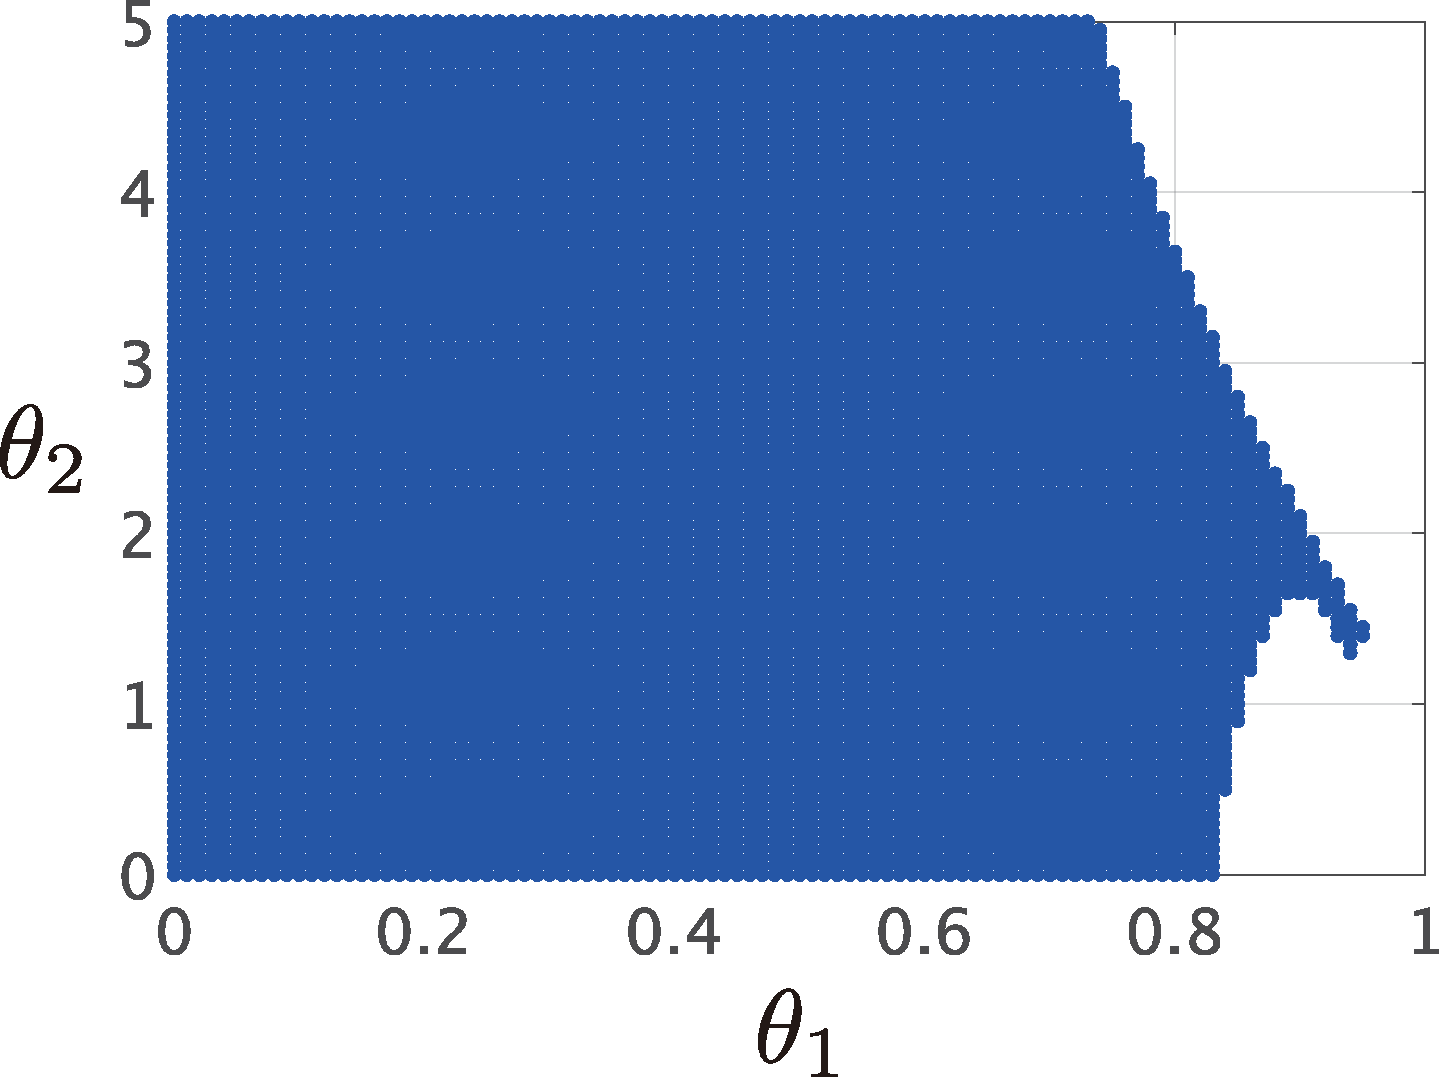
\includegraphics[width = 0.90\linewidth]{figs/Y0.01D1}
    \subcaption{$D=(10,10,10)$, $\bm{Y}=\tfrac{\bm{Y}_0}{100}$ }
    \medskip
  \end{minipage}
  \begin{minipage}{0.49\linewidth}
    \centering
    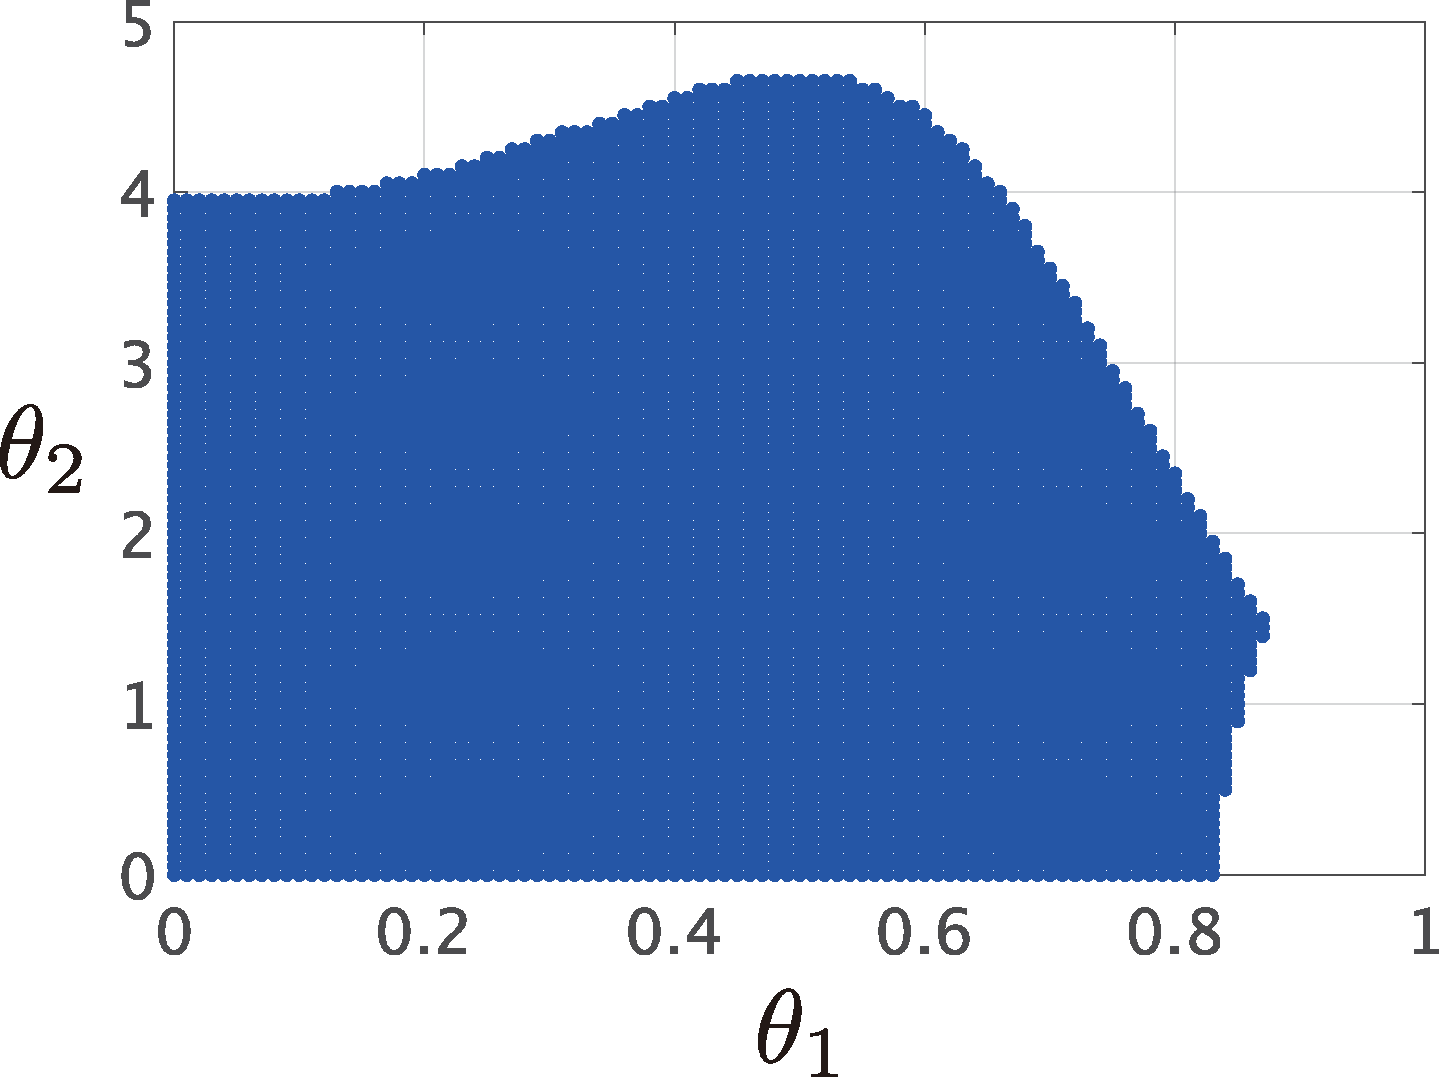
\includegraphics[width = 0.90\linewidth]{figs/Y0.01D0.01}
    \subcaption{$D=(\tfrac{1}{10},\tfrac{1}{10},\tfrac{1}{10})$, $\bm{Y}=\tfrac{\bm{Y}_0}{100}$}
    \medskip
  \end{minipage}
}
% \medskip
 \caption{\textbf{Area of parameters where the approximate linear model is stable}}
 \label{fig:stacheck}
\medskip
\end{figure}


\section{Mathematical stability analysis of the linearized
model\advanced}\label{sec:linmathana}

\subsection{Small signal stability of the linearized model\advanced}
In this section, we mathematically analyze the stability of the linearized model
given in equation \ref{eq:lindynu0}. The stability is characterized by the
eigenvalues of the matrix $\Psi$. However, as discussed in section
\ref{sec:numlinsta}, $\Psi$ is not regular and the eigenspace for the zero
eigenvalue is given by

\begin{equation}\label{eq:eqset}
  \mathcal{M} =
  \sfspan\left\{
  \mat{
  \mathds{1}\\
  0\\
  0
  }
  \right\}
\end{equation}
%\footnote{
%正方行列$A$のある固有値$\lambda$に対して
%\[
%\mathcal{V}_{\lambda}:= \sfker (\lambda I -A)
%\]
%を$\lambda$に対する\emph{固有空間}(eigenspace)と呼ぶ。
%固有値$\lambda$に対するすべての線形独立な固有ベクトルを$v_1,\ldots,v_k$とするとき
%\[
%\mathcal{V}_{\lambda} = \sfspan\{v_1,\ldots,v_k\}
%\]
%が成り立つ。
%すなわち,特定の固有値に対する固有ベクトルが張る線形空間である。
%}
%。
This eigenspace represents the set of equivalent steady-state values obtained by
varying the phase angles of all generators while maintaining their relative
values constant. Therefore, it is not a problem which point in the equilibrium
set of Equation \ref{eq:eqset} the state of the approximate linear model
converges to. Based on this fact, we give the following definition:

\begin{COLUMN}
\noindent \textbf{Eigenspace of a square matrix}:
For a square matrix $A$ and a given eigenvalue $\lambda$, the \emph{eigenspace}
\index{eigenspace} $\mathcal{V}_{\lambda}$ is defined as:

\[
  \mathcal{V}_{\lambda}:= \sfker (\lambda I -A)
\]
where $\sfker$ denotes the kernel of the matrix. If $v_1,\ldots,v_k$ are all
linearly independent eigenvectors corresponding to a specific eigenvalue
$\lambda$, then:

\[
\mathcal{V}_{\lambda} = \sfspan\{v_1,\ldots,v_k\}
\]
which means that it is a linear space spanned by the eigenvectors associated
with a specific eigenvalue.

\end{COLUMN}


\begin{definition}[Small-signal stability of the linear approximation model]
\label{def:stalin}

Consider the linearized model given by Equation \ref{eq:lindynu0}. For any
initial values, if the internal state converges to one of the equilibrium points
in the set $\mathcal{M}$ defined by Equation \ref{eq:eqset}, the linearized
model is said to be \textbf{steady-state stable}\index{steady-state stability}.
%\footnote{
%電力系統工学では,微小な外乱に対する電力系統の安定性を近似線形モデルを用いて議論する場合に広く「定態安定性」という用語が用いられる。
%ただし,definition\ref{def:stalin}のように数学的なdefinitionを導入することは一般的ではない。
%}。
\end{definition}
The small-signal stability in Definition \ref{def:stalin} means that for any
initial condition, Equation \ref{eq:linmconv} holds. Note that the value of
$c_0$ in Equation \ref{eq:linmconv} is arbitrary, so we express its
arbitrariness as "converging to one of the equilibrium points in $\mathcal{M}$."

In power system engineering, the term "small-signal stability" is widely used to
discuss the stability of a power system against small disturbances using an
approximate linear model. However, introducing a mathematical definition like
Definition \ref{def:stalin} is not common practice.

In the following discussion, we assume that the kernel space of $\Psi$ in
Equation \ref{eq:lindynu0} is one-dimensional and that Equation
\ref{eq:nesconker} holds:
\begin{equation}\label{eq:nesconker}
  \sfker \Psi = \mathcal{M}
\end{equation}
It is clear from the structure of the matrix $\Psi$ that $\mathcal{M}$ is a
subset of $\sfker \Psi$, but it should be noted that we are assuming that
$\sfker \Psi$ is one-dimensional and that the equality holds. If the kernel
space were two-dimensional or greater, the invariant eigenspace would be larger
than $\mathcal{M}$, and the approximate linear model would not be in a steady
state stability.
%\footnote{
%行列$\Psi$の構造から,$\mathcal{M} \subseteq \sfker \Psi $であることは明らかであるが,ここでは$\sfker \Psi$が1次元であり,等号が成り立つことを仮定している。
%この核空間が2次元以上であると,不変な固有空間が$\mathcal{M}$よりも大きくなり,近似線形モデルは定態安定とならない。
%}
%。
Therefore, equation \ref{eq:nesconker} is a necessary condition for the
steady-state stability of the linear approximation model. In particular, when
$A$ is invertible, and using the definition of $L_0:= L-CA^{-1}B$, the
necessary condition can be equivalently expressed as:
\begin{equation}\label{eq:nescon}
  \sfker L_0 = \sfspan
  \left\{
  \mathds{1}
  \right\}
\end{equation}
Note that this matrix $L_0$ plays an important role in the subsequent analysis.

The relationship between equation \ref{eq:defL0} and equation \ref{eq:nescon}
can be verified as follows. Because the $(1,2)$ block of the matrix $\Psi$ is
invertible, the necessary and sufficient condition for the kernel of $\Psi$ to
be equal to $\mathcal{M}$ is:

\begin{equation*}%\label{eq:nescon0}
  \sfker \mat{
  -L & -C \\
  B & A
  }
  = \sfspan
  \left\{
  \mat{
  \mathds{1}\\
  0
  }
  \right\}
\end{equation*}

In particular, when $A$ is invertible, we have
\begin{align*}
\mat{
-L & -C \\
B & A
}\mat{x\\y}
=0
\qquad
\Longleftrightarrow
\quad
L_0 x=0,
\qquad
y=-A^{-1}Bx
\end{align*}
Thus, the necessary condition is equivalent to equation \ref{eq:nescon}.

For the following discussion, we introduce the following fundamental
terminology.

\begin{definition}[Stability of square matrix]
\label{def:matsta}
For a square matrix $A$, if all the real parts of its eigenvalues are negative,
$A$ is called \textbf{stable}\index{stable} or \textbf{asymptotically
stable}\index{asymptotically stable}.
\end{definition}

\subsection{Passivity of approximate linear models\advanced}\label{sec:linpasana}

\smallskip
\subsubsection{Representation of Approximate Linear Models with Feedback}

\begin{figure}[t]
\centering
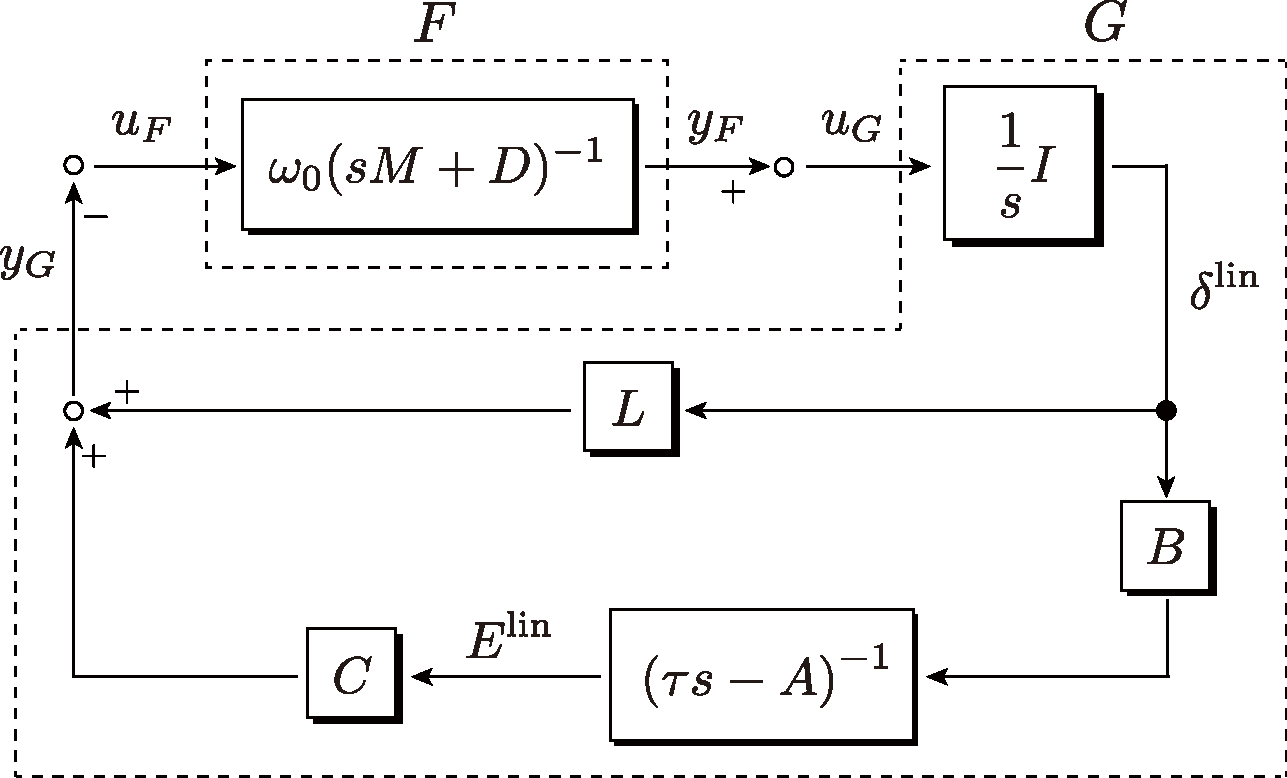
\includegraphics[width = .7\linewidth]{figs/FandG}
\medskip
\caption{\textbf{Feedback system representation of approximate linear models}}
\label{fig:GandG}
\medskip
\end{figure}

Let us consider describing the approximate linear model of Equation
\ref{eq:lindynu0} as a feedback system of two subsystems (Figure
\ref{fig:GandG}).  The first subsystem is described as a system of differential
equations for the deviation of the angular frequency:

\begin{equation}\label{eq:Fss}
  F: \simode{
  M \Delta \dot{\omega}^{\rm lin} &= -D \Delta \omega^{\rm lin}
  +
  u_F \\
  y_F &= \omega_0 \Delta \omega^{\rm lin}
  }
\end{equation}

In this book, we refer to this subsystem as the \textbf{mechanical
subsystem}\index{mechanical subsystem}. The mechanical subsystem is determined
solely by the physical constants of the generator set $(M_i, D_i){i \in
\mathcal{I}\text{G}}$ and the reference angular frequency $\omega_0$, and does
not depend on the steady-state values of the internal state $(\delta^{\star},
E^{\star})$.

The second subsystem is described as a system of differential equations with
respect to the rotor angle and internal voltage as follows:
\begin{equation}\label{eq:Gss}
  G: \simode{
  \dot{\delta}^{\rm lin} & = u_G \\
  \taud \dot{E}^{\rm lin} &= A E^{\rm lin} + B \delta^{\rm lin} \\
  y_G &= C E^{\rm lin} + L \delta^{\rm lin}
  }
\end{equation}

We call this subsystem the \textbf{electrical subsystem}\index{Electrical
subsystem} \footnote{The terms "mechanical subsystem" and "electrical subsystem"
introduced here are unique to this book.}.  The electrical subsystem not only
depends on the physical constants of the generator group, $(\taudi){i\in
\mathcal{I}{\rm G}}$, but also on the steady-state values of the internal
states, $(\delta^{\star},E^{\star})$. In fact, the system matrix $(L,A,B,C)$ in
equation \ref{eq:sysmats} is a function of $(\delta^{\star},E^{\star})$.

If the two subsystems' inputs and outputs are coupled through negative feedback
as follows:
\begin{align}\label{eq:nfedcon}
  u_F = -y_G,\qquad
  u_G = y_F
\end{align}
the approximate linear model of Equation \ref{eq:lindynu0} is represented. The
subsequent analysis of steady-state stability is based on the property called
the \textit{passivity} of the mechanical and electrical subsystems. It is
well-known that a negative feedback system of a passive subsystem is stable.

\smallskip
\subsubsection{Passivity of the mechanical subsystem}

The mechanical subsystem $F$ in Equation \ref{eq:Fss} has the following strong
passivity:

\begin{definition}[Passivity of linear systems]\label{def:passivelin}

Consider the linear system
\begin{equation}\label{eq:siglin}
  \Sigma: \simode{
  \dot{x} &= Ax + Bu \\
  y &= Cx 
  }
\end{equation}

Using the symmetric matrix $P$, define the function:
\begin{equation}\label{eq:defstlin}
  W(x):= \frac{1}{2}x^{\sf T}Px
\end{equation}

For any $u$, if there exists a semi-positive definite matrix $P$ that satisfies:
\begin{align}\label{eq:conpvlin}
\frac{d}{dt} W\bigl( x(t) \bigr) \leq u^{\sf T}(t) y(t)
,\qquad
\forall t \geq 0
\end{align}
Then, we call $\Sigma$ \textbf{passive}\index{passive}.

In particular, when there exists a positive definite number $\rho$ such that in
addition to the semi-positive definite matrix, the inequality:
\begin{align}\label{eq:conosplin}
\frac{d}{dt} W\bigl( x(t) \bigr) \leq u^{\sf T}(t) y(t) -\rho \left\|y(t) \right\|^2
,\qquad
\forall t \geq 0
\end{align}
is satisfied, then we call $\Sigma$ \textbf{strictly passive}\index{strictly
passive}.

\end{definition}

The function $W(x)$ in Definition \ref{def:passivelin} is generally called the
\textbf{storage function}\index{storage function}. Moreover, the inequality in
Equation \ref{eq:conosplin} describes a type of passivity that is more strictly
called \textbf{output-strict passivity}\index{output-strict passivity}, where
the energy represented by the storage function $W(x)$ dissipates more quickly in
proportion to the square of the output compared to the passivity in Equation
\ref{eq:conpvlin}.

The mechanical subsystem $F$ of Equation\ref{eq:Fss} having strong passivity can
be confirmed as follows. First, the subsystem is written as below:
\begin{align}
  F: \simode{
  \dot{x}_F & = A_F x_F + B_F u_F \\
  y_F &= C_F x_F
  }
\end{align}
where state $x_F$ represents $\Delta \omega^{\rm lin}$, and the system matrices
are:
\[
  A_F := -M^{-1}D,\qquad
  B_F := M^{-1},\qquad
  C_F := \omega_0 I
\]

Additionally, we define the symmetric matrix $P_F$ as:
\[
  P_F := \omega_0 M
\]
and since $M$ is positive definite, $P_F$ is also positive definite.
Then, the following inequalities hold:

\[
  A^{\sf T}_F P_F + P_F A_F \preceq  
  - \frac{ 2 \sfmin \left\{ D_i \right\}}{\omega_0} C_F^{\sf T} C_F
  ,\qquad
  P_F B_F = C_F^{\sf T}
\]

Therefore, when the storage function is defined as:
\begin{align}\label{eq:WFdef}
W_F(x_F):= \frac{1}{2}x_F^{\sf T}P_Fx_F
\end{align}
the time derivative along the solution trajectory of $F$ is evaluated as:

\begin{align}\label{eq:Flyapeq}
\spliteq{
\frac{d}{dt} W_F \bigl( x_F (t) \bigr)
& = 
\nabla W_F^{\sf T}(x_F) \frac{d x_F}{dt} 
 \\
&=  \bigl( P_F x_F(t) \bigr)^{\sf T} \bigl(A_F x_F(t) + B_F u_F(t) \bigr) \\
 & = y_F^{\sf T}(t) u_F(t)
 + \frac{1}{2} x_F^{\sf T}(t) \left(A^{\sf T}_F P_F + P_F A_F\right) x_F(t) \\
& \leq 
y_F^{\sf T}(t) u_F(t)
- \tfrac{\sfmin \left\{ D_i \right\}}{\omega_0}
\|y_F(t) \|^2
}
\end{align}
where $\nabla W_F(x_F)$ is the gradient function obtained by partially
differentiating $W_F(x_F)$ with respect to its elements and arranging them
vertically. From this, it can be seen that the machine subsystem $F$ in Equation
\ref{eq:Fss} is strongly passive for any positive definite $(M_i,D_i)_{i \in
\mathcal{I}_{\rm G}}$. Note that the function $W_F(x_F)$ represents the
mechanical kinetic energy of the power system.

\smallskip
\subsubsection{Passivity of an electrical subsystem}
Next, let us consider the electrical subsystem of Equation \ref{eq:Gss}.
Unlike the mechanical subsystem $F$, the electrical subsystem $G$ only has passivity under limited conditions.
Though this comes out of nowhere, let us consider a case where reduced conductance of Equation \ref{eq:figi} is all 0; in other words:
\begin{align}\label{eq:Gredcon}
G^{\rm red}_{ij}=0,\qquad 
\forall (i, j) \in \mathcal{I}_{\rm G} \times \mathcal{I}_{\rm G}
\end{align}

Excluding special situations, the conditions of Equation \ref{eq:Gredcon} only hold when the conductance of all transmission lines in an electrical power system is 0; in other words, the resistance of all transmission lines is 0.
At this time, the following is true for the function $k_{ij}(\delta_{ij})$,$h_{ij}(\delta_{ij})$ of Equation \ref{eq:defkh}:
\begin{align*}
k_{ij}(\delta_{ij}^{\star}) =
k_{ji}(\delta_{ji}^{\star})
,\qquad
h_{ij}(\delta_{ij}^{\star}) = 
- h_{ji}(\delta_{ji}^{\star}),\qquad
h_{ii}(\delta_{ii}^{\star}) = 0
\end{align*}

Therefore, the following is true for the system matrix of $(L,A,B,C)$ of Equation \ref{eq:sysmats}.
\begin{align}\label{eq:sysmatst}
L=L^{\sf T} ,\qquad
\hat{A} = \hat{A}^{\sf T},\qquad
C= -\hat{B}^{\sf T}
\end{align}
Below, we analyze the passivity of an electrical subsystem by using a symmetrical structure of a special system matrix. 

First, let us express the electrical subsystem $G$ of Equation \ref{eq:Gss} as follows:
\begin{align}
G: \simode{
\dot{x}_G & = A_G x_G + B_G u_G \\
y_G &= C_G x_G
}
\end{align}

where state $x_G$ is a column vector with ${\delta}^{\rm lin}$ and $ E^{\rm lin} $,
where a system matrix is expressed as below using a diagonal matrix that is positive definite:
\[
 \Omega :=
\sfdiag \left( \sqrt{\frac{ \Xsi - \Xti }{ \taudi } } \right)_{i \in \mathcal{I}_{\rm G} }
\]
The symmetric matrix $P_G$ is defined as:
\[
A_G := 
\mat{
0 & 0 \\
 \Omega^2 \hat{B}   &  \Omega^2 \hat{A} 
},\qquad
B_G := 
\mat{
I \\
0
},\qquad
C_G := 
\mat{
L & -\hat{B}^{\sf T}
}
\]
For these matrices, the following is true:
\begin{align}\label{eq:defPG}
P_G := 
\mat{
L  &  - \hat{B}^{\sf T} \\
- \hat{B} & -\hat{A}
}
\end{align}
The fact that the left matrix inequality holds can be confirmed as follows:
\begin{align}\label{eq:lyapinG}
A^{\sf T}_G P_G + P_G A_G \preceq 
0
,\qquad
P_G B_G = C_G^{\sf T}
\end{align}

If we calculated the left of the inequality, it can be expressed as follows using a symmetric matrix $\hat{A}_{\Omega} := \Omega \hat{A} \Omega$:
\[
\frac{
A^{\sf T}_G P_G + P_G A_G
}{2}
=
\mat{
\Omega \hat{B} & 0\\
0 &\Omega^{-1}
}^{\sf T}
\underbrace{
\mat{
-I & -\hat{A}_{\Omega} \\
-\hat{A}_{\Omega} & - \hat{A}_{\Omega}^2
}
}_{Y}
\mat{
\Omega \hat{B} & 0\\
0 & \Omega^{-1}
}
\]

Since the top left block $- I$ of $Y$ is negative definite and the Schur complement related to $-I$ of $Y$ is 0, $Y$ is negative semi-definite.
\begin{COLUMN}
\noindent \textbf{Shur complement}:
The symmetric matrix $M$ is sorted as follows:
\[
M =\mat{
M_{11} & M_{12} \\
M_{12}^{\sf T} & M_{22}
}
\]
At this time:
\[
M/M_{22} := M_{11} - M_{12} M_{22}^{-1} M_{12}^{\sf T}
\]
is called the \textbf{Schur complement} related to $M_{22}$ of $M$.
Similarly, 
\[
M/M_{11} := M_{22} - M_{12}^{\sf T} M_{11}^{-1} M_{12}
\]
is called the Schur complement related to $M_{11}$ of $M$.
When matrix $M_{22}$ is positive definite, the condition necessary for $M$ to be positive semi-definite is for $M/M_{22}$ to be positive semi-definite.
A similar fact is true for $M/M_{11}$\cite{bernstein2009matrix}.
In addition, it is true when a positive semi-definite is replaced with a positive definite.

\smallskip
\noindent \textbf{Properties of semidefinite matrices}:
For negative semi-definite matrix $Y\in \mathbb{R}^{n\times n}$ and arbitrary matrix $X\in \mathbb{R}^{n\times m}$, $X^{\sf T}YX$ is negative semi-definite.
This can be confirmed by:
\[
v^{\sf T}Yv\geq 0, \quad \forall v\in \mathbb{R}^n
\qquad
\Longrightarrow
\qquad
(Xw)^{\sf T} Y (Xw) \geq 0, \quad \forall w\in \mathbb{R}^m
\]
\end{COLUMN}

Using the relationship of Equation \ref{eq:lyapinG}, the time derivative of the storage function: 
\begin{align}\label{eq:WGdef}
W_G(x_G):= \frac{1}{2}x_G^{\sf T}P_Gx_G
\end{align}
along with the solution trajectory of $G$ can be assessed as below in the same way as Equation \ref{eq:Flyapeq}: 
\begin{align}\label{eq:Glyapeq}
\frac{d}{dt} W_G \bigl( x_G (t) \bigr)
 \leq 
y_G^{\sf T}(t) u_G(t)
\end{align}
However, to show the passivity of $G$, $P_G$ of Equation \ref{eq:defPG} must be positive semi-definite.
Here, if the matrix $A$ of Equation \ref{eq:sysmats} is stable:
\[
A= S^2 \hat{A}
\qquad \Longleftrightarrow \qquad S^{-1} A S = S \hat{A} S
\]
Thus, eigenvalues of $S \hat{A} S$ are all negative.
However:
\[
S:=\sfdiag \left( \sqrt{ \Xsi -  \Xti }\right)_{i \in \mathcal{I}_{\rm G} } 
\]
This means that $ \hat{A} $ is negative definite.
A condition necessary for $P_G$ of Equation \ref{eq:defPG} to be positive semi-definite is that the Schur complement related to $ -\hat{A} $ is positive semi-definite; in other words, the following is true:
\begin{align}\label{eq:pdsp}
L_0 =L_0^{\sf T} \succeq 0
\end{align}
However, for $L_0$ of Equation \ref{eq:defL0}, we used the fact that:
\[
L_0 = L + \hat{B}^{\sf T} \hat{A}^{-1} \hat{B}
\]
from Equation \ref{eq:sysmatst}.
To summarize the above discussion, the following term is introduced.

\begin{definition}[Passive power transmission conditions]\label{def:passtrans}
For the system matrix $(L,A,B,C)$ of Equation \ref{eq:sysmats}, the following three conditions are together called \textbf{passive power transmission conditions}.
\footnote{
“Passive power transmission conditions” is a term unique to this book.
}。
\begin{itemize}
\item[(i)] Matrix $A$ is stable.
\item[(ii)] As in Equation \ref{eq:Gredcon}, reduced conductance is all 0.
\item[(iii)] For the matrix $L_0$ of Equation \ref{eq:defL0}, the matrix inequality of Equation \ref{eq:pdsp} hold. 
\end{itemize}
Individually, it may be called a passive power transmission condition (i), and so on.
\end{definition}

Based on the above discussions, we can see that the passive power transmission conditions describe the conditions necessary for the electrical system $G$ of Equation \ref{eq:Gss} to be passive.
Furthermore, these conditions are necessary for the linear approximation model to be statically stable for the passivity of an electrical subsystem and arbitrary physical constant.
The details are discussed in Section \ref{sec:nesconana} and Section \ref{sec:nesconsta}.
Function $W_G(x_G)$ indicates the electrical potential energy of an electrical power system.

\subsection{Analysis of small signal stability based on passivity\advanced}

\smallskip
\subsubsection{Stability analysis for a feedback system}

Below, when an electrical subsystem is passive under the passive power transmission conditions of definition \ref{def:passtrans}, the stability of their feedback system, in other words, the small signal stability of the linear approximation model of Equation \ref{eq:lindynu0}, is analyzed.
Since the inequality of Equation \ref{eq:Flyapeq} and Equation \ref{eq:Glyapeq} holds, the sum is:
\smallskip
\begin{align*}
\spliteq{
 \frac{d}{dt} \bigl\{ W_F \bigl( x_F (t) \bigr)
& +
 W_G \bigl( x_G (t) \bigr)
 \bigr\} \\
& \leq 
\underbrace{
y_F^{\sf T}(t) u_F(t)
+
y_G^{\sf T}(t) u_G(t)
}_{\star}
- \tfrac{\sfmin \left\{ D_i \right\}}{\omega_0}
\|y_F(t) \|^2
}
\end{align*}
If the equation of the feedback connection of Equation \ref{eq:nfedcon} is substituted into this inequality,
the term shown in “$\star$” is cancelled, and as the inequality for the entire feedback system,
the following is obtained:
\begin{align}\label{eq:FGlyapeq}
 \frac{d}{dt} \bigl\{ W_F \bigl( x_F (t) \bigr)
 +
 W_G \bigl( x_G (t) \bigr)
 \bigr\} 
 \leq 
- \tfrac{\sfmin \left\{ D_i \right\}}{\omega_0}
\|y_F(t) \|^2
\end{align}
In other words, the sum of function $W_F(x_F)$ and function $W_G(x_G)$ is monotonous non-increasing with the temporal changes along the solution trajectory of the feedback system.
Since the lower limits of $W_F(x_F)$ and $W_G(x_G)$ are 0, when enough time passes, the sum asymptotically converges to a value.
This means that the time derivative on the left of Equation \ref{eq:FGlyapeq} asymptotically converges to 0.
The right side of Equation \ref{eq:FGlyapeq} is negative when $y_F(t)\neq 0$, and 0 only when $y_F(t)=0$; thus, the following is obtained:
\begin{align}\label{eq:yFlim0}
\lim_{t\rightarrow \infty} y_F(t)  =0
\end{align}
Furthermore, if we focus on the output equation of Equation \ref{eq:Fss}, the output $y_F$ is a constant factor of the internal state $\Delta \omega^{\rm lin}$; 
thus, the following holds for the mechanical subsystem $F$:
\begin{align}\label{eq:Fobs}
y_F(t)  =0,\quad \forall t\geq 0 
\qquad \Longrightarrow \qquad
\Delta \omega^{\rm lin}(t)  =0,\quad \forall t\geq 0 
\end{align}
This is a property called \textbf{observability} in control systems engineering.
Therefore, from Equation \ref{eq:yFlim0} and Equation \ref{eq:Fobs}, we can see that the following
is true for the arbitrary initial value $(\Delta \omega^{\rm lin}(0),\delta^{\rm lin}(0),E^{\rm lin}(0))$ for the linear approximation model of Equation \ref{eq:lindynu0}:
\begin{align}\label{eq:Delom0}
\lim_{t\rightarrow \infty} \Delta \omega^{\rm lin}(t)  =0
\end{align}
In other words, the internal state of the mechanical subsystem $F$ of Equation \ref{eq:Fss} in a feedback system that asymptotically converges to 0.

\begin{COLUMN}
\noindent \textbf{Observability}:
For the linear system $\Sigma$ of Equation \ref{eq:siglin}, if the output $y(t)$ is identically 0 and the internal state $x(t)$ is also identically 0, $\Sigma$ is called \textbf{observable}.
Conditions necessary for $\Sigma$ to be observable are:
\begin{align}\label{eq:condobs}
\sfker \mat{
C \\
CA \\
\vdots \\
CA^{n-1}
}
=\{0\}
\end{align}
where $n$ is the dimension of the state.
By context, a pair of matrices satisfying the Equation \ref{eq:condobs} is called an observable pair $(C,A)$.

\smallskip
\noindent \textbf{Controllability}:
For the linear system $\Sigma$ of Equation \ref{eq:siglin}, if there is an input $u(t)$, where $x(T) = 0$ for a certain time $T > 0$ for each and every initial value $x(0)$, $\Sigma$ is called \textbf{controllable}.
Conditions necessary for $\Sigma$ to be controllable are:
\begin{align}\label{eq:condcon}
\sfim \mat{
B & AB & \cdots &A^{n-1}B
}
= \mathbb{R}^n
\end{align}
where $n$ is the dimension of the state. $\sfim$ expresses the \textbf{image} of a matrix
Depending on the context, a pair of matrices satisfying the Equation \ref{eq:condcon} is called a controllable pair $(A,B)$.

\smallskip
\noindent \textbf{Lyapunov function}:
Let us consider an observable linear system $\Sigma$ of Equation
\ref{eq:siglin}. However, the input $u(t)$ is identically 0. In addition, we
consider a positive semi-definite value function that satisfies $V(x)\geq0$ for
arbitrary $x$ and $V(x)=0$. If there is a positive definite number $\rho$, and:
\[
\frac{d}{dt} V \bigl( x (t) \bigr) 
=
\nabla V^{\sf T}(x) \frac{d x}{dt} (t)
\leq  - \rho \|y(t)\|^2,\qquad
\forall t \geq0
\]
is true for the differential along the solution trajectory of $\Sigma$ of function $V(x)$, the solution trajectory $x(t)$ for the arbitrary initial value asymptotically converges to 0.
This function $V(x)$ is called the \textbf{Lyapunov function}.

\begin{figure}[h]
\centering
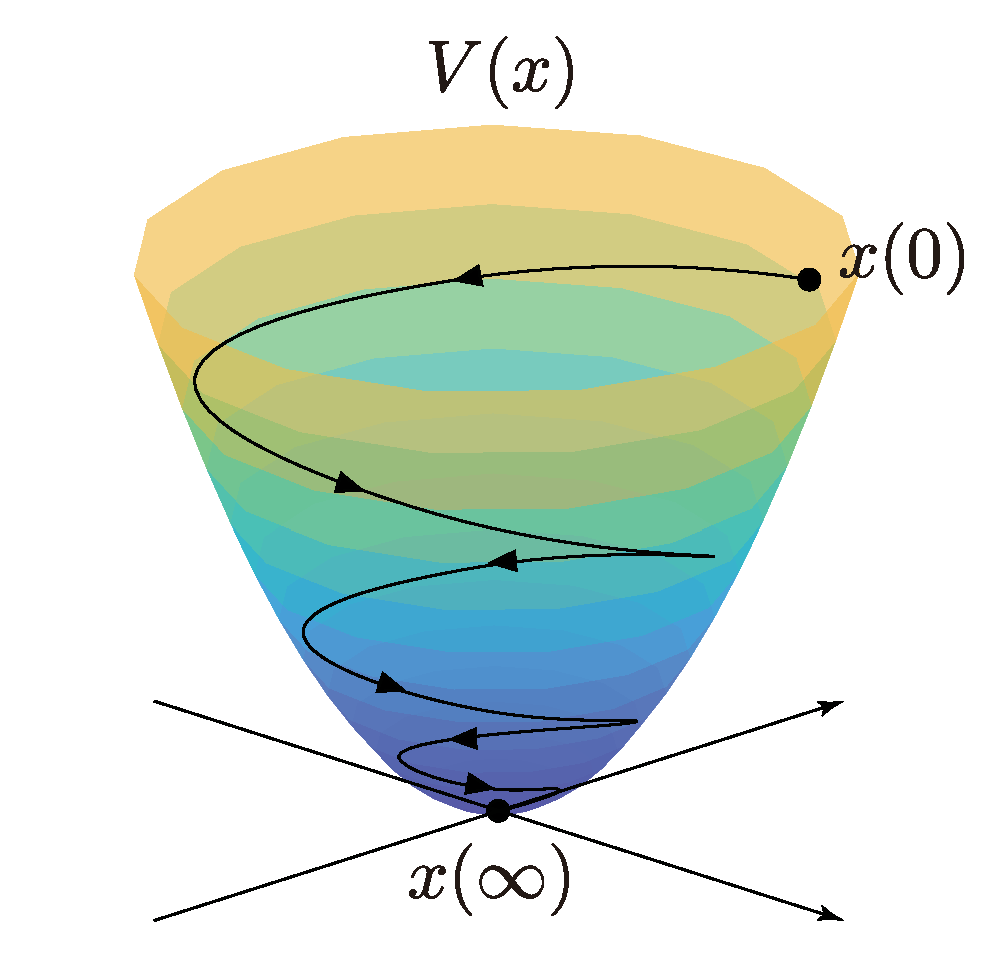
\includegraphics[width = .35\linewidth]{figs/cone}
\caption{\textbf{Monotonically decreasing values along the solution trajectory of the Lyapunov function}}
\label{fig:conelyap}
\medskip
\end{figure}


The fact that the value of the Lyapunov function monotonically decreases along the solution trajectory of the system can be interpreted as some type of energy dissipating with time (Figure \ref{fig:conelyap}).
Stability analysis based on a similar argument can be applied to a nonlinear system as well.

\end{COLUMN}

On the other hand, the fact that the internal state of the electrical subsystem $G$ of Equation \ref{eq:Gss} asymptotically converges to 0 cannot be derived from the above argument.
Specifically, the following is derived for the input and output of two subsystems from asymptotic convergence of Equation \ref{eq:Delom0} and the relationship of Equation \ref{eq:nfedcon}:
\[
\lim_{t\rightarrow \infty} u_F(t)  =0,\qquad
\lim_{t\rightarrow \infty} u_G(t)  =0,\qquad
\lim_{t\rightarrow \infty} y_G(t)  =0
\]
However, since the electrical subsystem is not observable, we cannot conclude that its internal system asymptotically converges.
If we assume that the electrical subsystem is observable, for the arbitrary initial value: 
\[
\lim_{t\rightarrow \infty}  \delta^{\rm lin}(t)  =0,\qquad
\lim_{t\rightarrow \infty}  E^{\rm lin}(t)  =0
\]
This means that for Equation \ref{eq:linmconv}, it is always $c_0=0$.
This fact is inconsistent with the idea that $\Psi$ of Equation \ref{eq:lindynu0} has a zero eigenvalue and is unstable.
Excluding special situations, the electrical subsystem is controllable.


\begin{figure}[t]
  \centering
  {
  \begin{minipage}{0.49\linewidth}
    \centering
    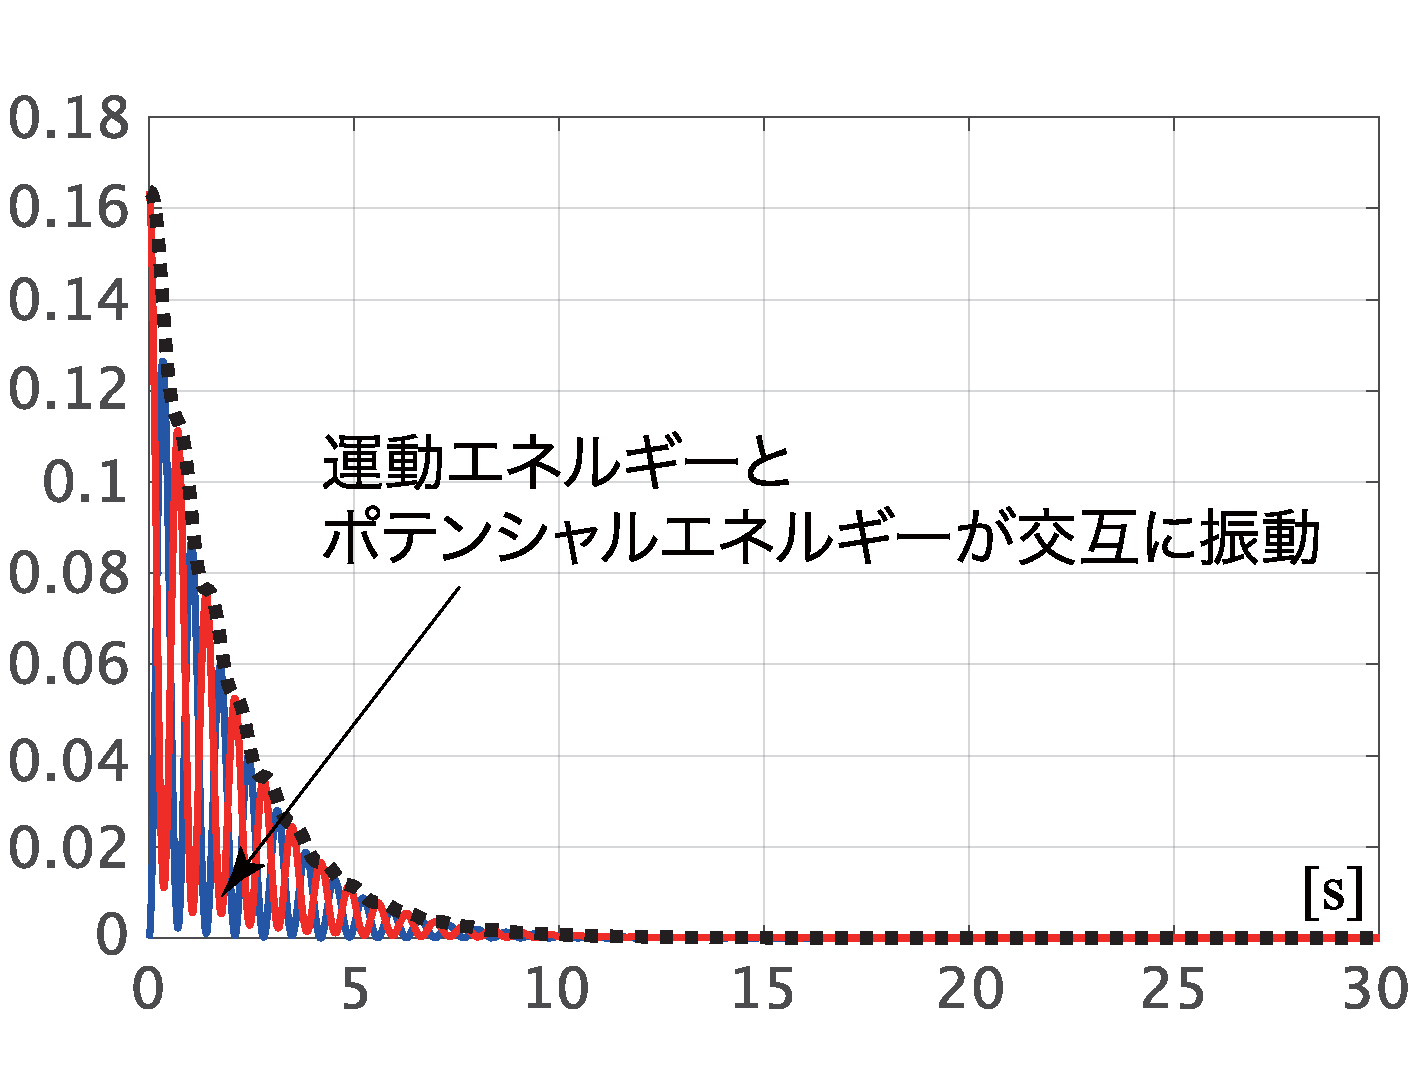
\includegraphics[width = 1.0\linewidth]{figs/losslessW}
    \subcaption{If passive transmission condition (ii) is met}
    \medskip
  \end{minipage}
  \begin{minipage}{0.49\linewidth}
    \centering
    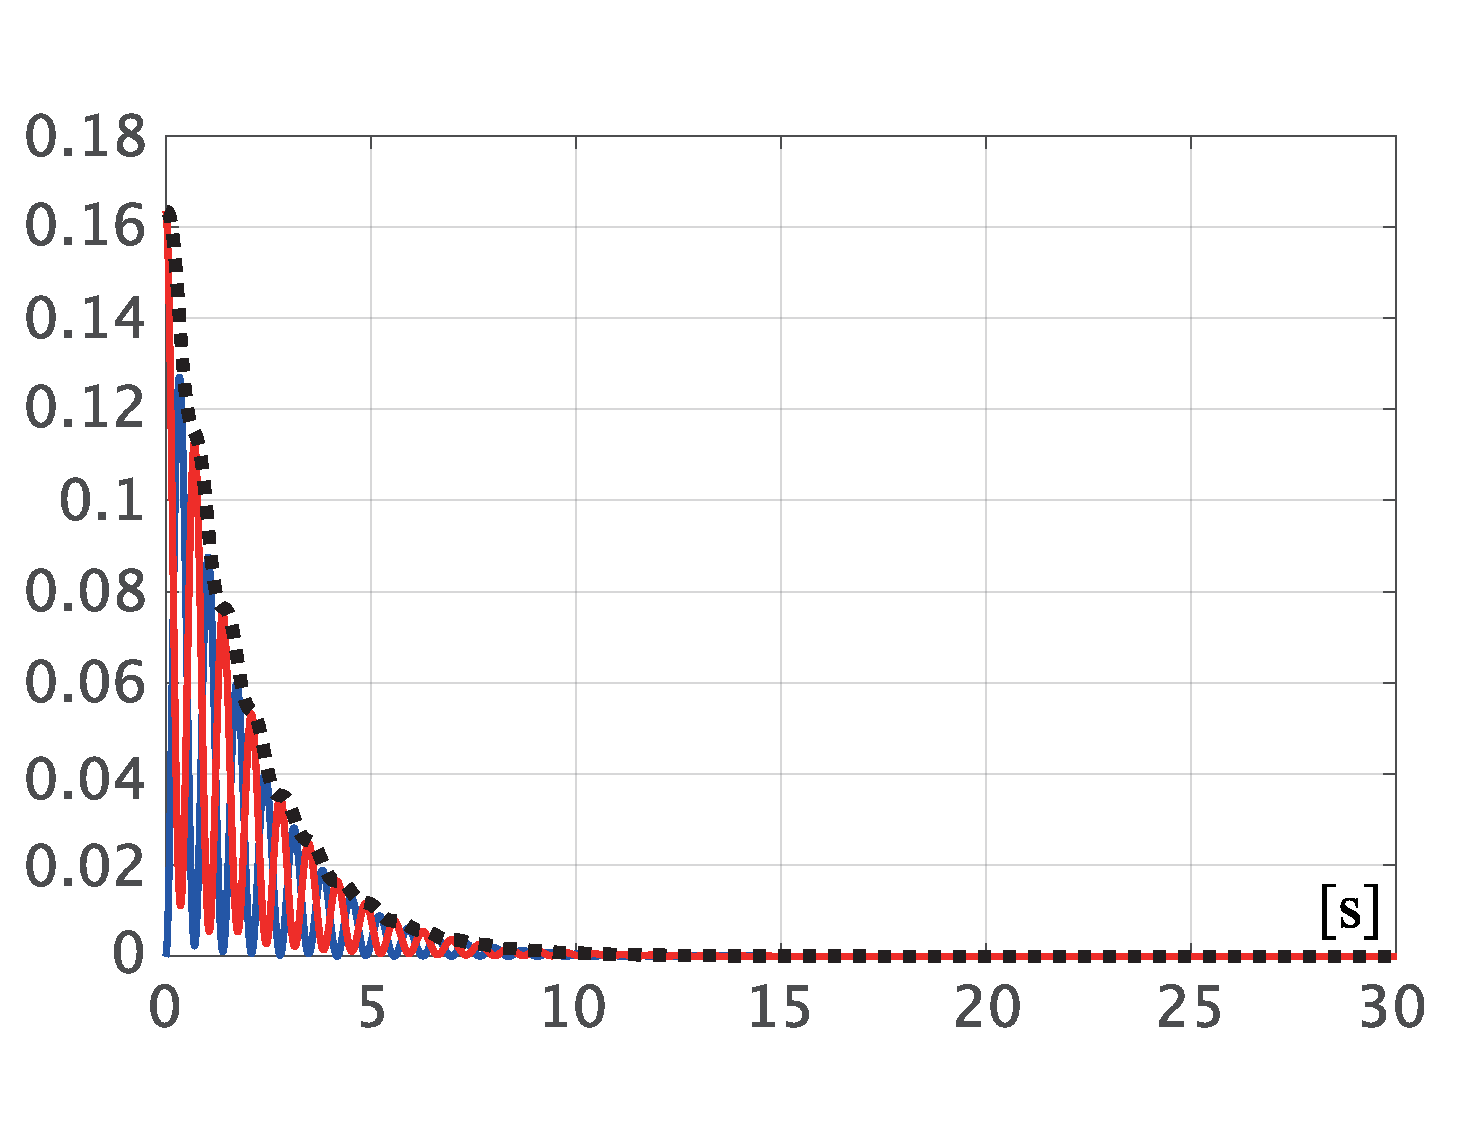
\includegraphics[width = 1.0\linewidth]{figs/lossyW}
    \subcaption{If passive transmission condition (ii) is not met}
    \medskip
  \end{minipage}
  }
  \medskip
  \caption{\textbf{Time variation of the accumulation function according to Example \ref{ex:linsyssim}}
  \\  \centering(Blue: $W_F$, Red: $W_G$, Black:$W_F+W_G$)}
  \label{fig:LyapW}
\medskip
\end{figure}


\begin{example}[Temporal change in accumulated energy]\label{ex:energylin}
Let us consider the linear approximation model discussed in the first half of the Example \ref{ex:linsyssim}.
First, let us consider a case where the passive power transmission condition (ii) is satisfied; in other words, the conductance of two transmission lines is 0.
Specifically, we set the admittance of the transmission line as:
\begin{align}\label{eq:bothlossless}
\bm{y}_{12} = - \bm{j} 11.6041, \qquad
\bm{y}_{23} =  - \bm{j} 10.5107
\end{align}
This corresponds to a case where parameter $\theta_2$ is 0 in Equation \ref{eq:Y0theta2}.
At this time, matrix $A$ is stable. All eigenvalues of $L_0$ in Equation \ref{eq:defL0} become non-negative.
In other words, this means that passive power transmission conditions (i) and (iii) hold. 

For the time response to the initial value of Equation \ref{eq:linmini}, we calculate the temporal change in the kinetic energy $W_F(x_F)$ of Equation \ref{eq:WFdef} and potential energy $W_G(x_G)$ of Equation \ref{eq:WGdef}.
The result is shown in Figure \ref{fig:LyapW}(a). The solid blue and red lines show $W_F(x_F)$ and $W_G(x_G)$, respectively.
The broken black line shows their sum. This figure shows that the kinetic and potential energy alternately increase and decrease, while their sum, the total energy of the entire system, monotonically decreases. 
The decrease of the total energy over time can be interpreted as energy loss via friction by the damping factor.

Next, as a reference, let us look at the result when the passive power transmission condition (ii) is not satisfied.
Specifically, we set $\bm{Y}_0(1)$ as the admittance matrix $\bm{Y}$ for Equation \ref{eq:Y0theta2}, where $\theta_2$ is 1.
This is equivalent to calculating the temporal changes in the kinetic and potential energy against the initial response of Figure \ref{fig:timeex}.
If the passive power transmission condition (ii) is not satisfied, $P_G$ of Equation \ref{eq:defPG} is not a symmetric matrix, but potential energy $W_G(x_G)$ is calculated by using the definition of Equation \ref{eq:WGdef} as is.
The calculation result Figure \ref{fig:LyapW}(b) is almost the same as Figure \ref{fig:LyapW}(a).
This fact indicates that even when the conductance of the transmission lines is not 0, the electrical potential energy can be approximated based on the definition of Equation \ref{eq:WGdef}.
\end{example}

\smallskip
\subsubsection{Change of basis that separates unobservable state variables}

Let us consider deriving an observable subsystem by removing the common component of the unobservable rotor argument from the electrical subsystem $G$ of Equation \ref{eq:Gss}.
Specifically, by applying the change of basis to the state $\delta^{\rm lin}$ of Equation \ref{eq:lindyn}, a differential equation system that only describes the deviation of the rotor argument is derived.

\begin{COLUMN}
\noindent \textbf{Basis transformation of linear systems}:
The change in basis for a linear system is the following operation.
For the equation of state:
\[
\dot{x}(t)=Ax(t)+Bu(t)
\]
each element $x_i(t)$ of the $n$-dimensional state vector $x(t)$ expresses the
component when expanded by the basis $\{e_1,\ldots,e_n\}$:
\[
x(t)
=
e_1 x_1(t) + \cdots + e_n x_n(t)
\]
where $e_i$ is the $n$-dimensional vector where only the $i$th element has 1.
This basis is called the \textbf{standard basis}.
The equation of state expresses the temporal expansion of the “component” when the state vector is expressed with a certain basis.
Let us consider expressing this state vector $x(t)$ with a different basis $\{v_1,\ldots,v_n\}$;
in other words:
\[
x(t)
=
v_1 \xi_1(t) + \cdots + v_n \xi_n(t)
\]
where $\xi_i(t)$ is a component of the base vector $v_i$.
If a matrix with vectors $v_i$ in a row is $V$ and if a vector with $\xi_i(t)$ in a column is $\xi(t)$, it corresponds to a linear transformation called $x(t)=V\xi(t)$.
At this time, the equation of state is transformed to:
\[
\dot{\xi}(t)=V^{-1}AV \xi(t) + V^{-1} Bu(t)
\]
This differential equation system describes the temporal expansion of components with the new basis.
Note that the basis is divided into two parts like $\mathcal{V}_a:=\{v_1,\ldots,v_k\}$, $\mathcal{V}_b:=\{v_{k+1},\ldots,v_n\}$, and so on.
\[
x(t)=
V_{a} \xi_{a}(t) +
 V_{b} \xi_{b}(t)
\]
then the basis-transformed equation of state is:
\[
\mat{
\dot{\xi}_{a}(t) \\
\dot{\xi}_{b}(t)
}
=
\mat{
W_{a} A V_{a} & W_{a} A V_{b} \\
W_{b} A V_{a} & W_{b} A W_{b}
}
\mat{
{\xi}_{a}(t) \\
{\xi}_{b}(t)
}
\]
However, $V_{a}$ and $V_{b}$ are the matrices of the basis vectors of $\mathcal{V}_a$ and $\mathcal{V}_b$, and $W_{a}$ and $W_{b}$ are:
\[
\mat{
W_{a} \\
W_{b}
}
=\mat{
V_{a} & V_{b}
}^{-1}
\qquad
\Longleftrightarrow
\qquad
\mat{
V_{a} & V_{b}
}\mat{
W_{a} \\
W_{b}
}=I
\]
In this representation, $\xi_a(t)$ is the component of $x(t)$ with respect to the subspace $\sfspan \mathcal{V}_a$.
Also, $\xi_b(t)$ is a component with respect to $\sfspan \mathcal{V}_b$.
\end{COLUMN}

The change of basis explained below can be applied regardless of whether passive power transmission conditions hold.
$\delta^{\rm lin}$ is expanded using a matrix $W \in \mathbb{R}^{N\times (N-1)}$:
\begin{align}\label{eq:batrinv}
\delta^{\rm lin}
=
W
\delta^{\rm lin}_{\rm e} +
\mathds{1}
\overline{\delta}^{\rm lin}_{\rm e}
\end{align}
Here, $\mathds{1}$ is a base vector that expresses the common component of $\delta^{\rm lin}$, while $W$ is a matrix with base vectors that express other deviation components.
In other words, the common component of $\delta^{\rm lin}$ is $\overline{\delta}^{\rm lin}_{\rm e}$, and deviation components are $\delta^{\rm lin}_{\rm e}$.
The common component $\overline{\delta}^{\rm lin}_{\rm e}$ is one-dimensional, while deviation components $\delta^{\rm lin}_{\rm e}$ are $(N-1)$-dimensional.

Next, let us consider the inverse transformation of Equation \ref{eq:batrinv}.
Specifically, let us consider a matrix $W^{\dagger} \in \mathbb{R}^{(N-1)\times N}$:
\[
\delta^{\rm lin}
=
\underbrace{
\mat{
W & \mathds{1}
}
}_{T}
\mat{
\delta^{\rm lin}_{\rm e} \\
\overline{\delta}^{\rm lin}_{\rm e}
}
\quad
\Longleftrightarrow
\quad
\mat{
\delta^{\rm lin}_{\rm e} \\
\overline{\delta}^{\rm lin}_{\rm e}
}
=
\underbrace{
\mat{
W^{\dagger} \\
\frac{1}{N} \mathds{1}^{\sf T}
}
}_{T^{-1}}
\delta^{\rm lin}
\]
For this inverse transformation to exist, the column vector of $W$ must be orthogonal to $\mathds{1}$.
This can be confirmed as follows. From the relationship of inverse transformation:
\begin{align*}
T^{-1}T
=\mat{
W^{\dagger}W & W^{\dagger} \mathds{1}\\
\frac{1}{N} \mathds{1}^{\sf T} W & \frac{1}{N} \mathds{1}^{\sf T} \mathds{1}
}
=\mat{
I & 0\\
0 & 1
}
\end{align*}
must hold. In other words, $W$ and $W^{\dagger}$ are matrices that satisfy:
\[
\mathds{1}^{\sf T} W=0,\qquad
W^{\dagger}W=I,\qquad
W^{\dagger} \mathds{1}=0
\]
Therefore, from the first equation, we can see that the column vector of $W$ is orthogonal to $\mathds{1}$.
$W$ and $W^{\dagger}$ can be constructed by using an appropriate matrix, $U\in \mathbb{R}^{N\times (N-1)}$, that satisfies
\[
W = U(U^{\sf T}U)^{-1},\qquad
W^{\dagger}=U^{\sf T}
\]
At this time, the product $WW^{\dagger}$ is an orthogonal projection matrix to the orthogonal complement of $\sfspan\{\mathds{1}\}$; thus, this can be expressed as:
\begin{align}\label{eq:psudinv}
WW^{\dagger} = I - \frac{1}{N} \mathds{1} \mathds{1}^{\sf T}
\end{align}
Such a pseudo inverse matrix of $W$, $W^{\dagger}$, is called a \textbf{Moore-Penrose pseudoinverse}.

The concept of orthogonal projection is shown in Figure \ref{fig:orthogonal}.
The black arrow shows the space of $\sfspan\{\mathds{1}\}$, as the orthogonal complement $\sfspan\{\mathds{1}\}^{\perp}$, a plane that is orthogonal to the space.
If the vector $v$ is multiplied by orthogonal projection matrix $WW^{\dagger}$, $WW^{\dagger}v$ is obtained as an image projected perpendicular to $\sfspan\{\mathds{1}\}^{\perp}$ from $v$.
\[
I-WW^{\dagger}=\tfrac{1}{N}\mathds{1} \mathds{1}^{\sf T}
\]
in a complimentary relationship is an orthogonal projection matrix to $\sfspan\{\mathds{1}\}$.

\begin{figure}[t]
\centering
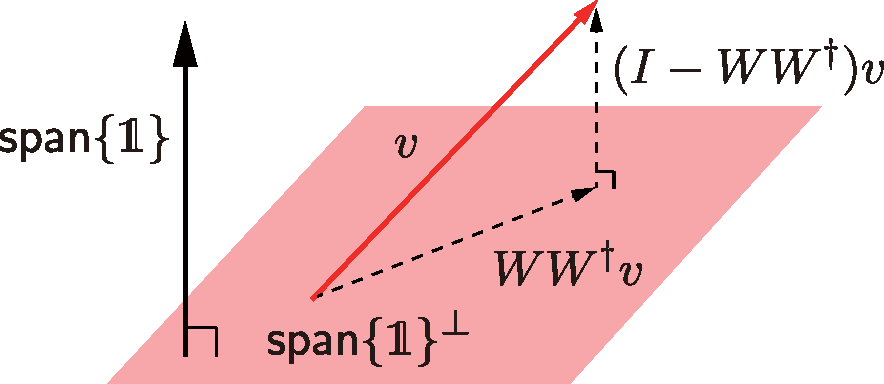
\includegraphics[width = .50\linewidth]{figs/orthogonal}
\medskip
\caption{\textbf{Conceptual diagram of orthogonal projection}}
\label{fig:orthogonal}
\medskip
\end{figure}

We apply the above-mentioned change of basis to the electrical subsystem $G$ of Equation \ref{eq:Gss}.
irst, if we substitute Equation \ref{eq:batrinv} into a differential equation related to $\delta^{\rm lin}$, the following is obtained:
\[
W
\dot{\delta}^{\rm lin}_{\rm e} +
\mathds{1}
\dot{\overline{\delta}}^{\rm lin}_{\rm e}=u_G
\]
If this differential equation is multiplied by $W^{\dagger}$ or $\tfrac{1}{N} \mathds{1}^{\sf T}$ from the left, the following is obtained:
\[
\dot{\delta}^{\rm lin}_{\rm e} = W^{\dagger} u_G,\qquad
\dot{\overline{\delta}}^{\rm lin}_{\rm e} = \frac{1}{N} \mathds{1}^{\sf T} u_G
\]
Next, if we pay attention such that the relationship of Equation \ref{eq:LBker} holds for matrices $L$ and $B$, the differential equation and output equation related to $E^{\rm lin}$ can be rewritten as:
\[
\taud \dot{E}^{\rm lin} = A E^{\rm lin} + 
B W {\delta}^{\rm lin}_{\rm e}
, \qquad
y_G = C E^{\rm lin} + 
L W {\delta}^{\rm lin}_{\rm e}
\]
Therefore, the electrical subsystem with a changed basis is obtained as:
\begin{align}\label{eq:Gsstr}
G: \simode{
\dot{\overline{\delta}}^{\rm lin}_{\rm e} & = \tfrac{1}{N} \mathds{1}^{\sf T} u_G \\
\dot{\delta}^{\rm lin}_{\rm e} & = W^{\dagger}u_G \\
\taud \dot{E}^{\rm lin} &= A E^{\rm lin} + B W {\delta}^{\rm lin}_{\rm e} \\
y_G &= C E^{\rm lin} + L W {\delta}^{\rm lin}_{\rm e}
}
\end{align}
What we need to focus on in this system expression is that ${\overline{\delta}}^{\rm lin}_{\rm e}$ that expresses the common component of $\delta^{\rm lin}$ is impacted by the input $u_G$, but not the output $y_G$.
In other words, ${\overline{\delta}}^{\rm lin}_{\rm e}$ is an unobservable state variable.

By removing the differential equation of ${\overline{\delta}}^{\rm lin}_{\rm e}$ from Equation \ref{eq:Gsstr}, $(N-1)$-dimensional controllable and observable subsystem is obtained as:
\begin{align}\label{eq:Gsstrmin}
G_{\rm e}: \simode{
\dot{\delta}^{\rm lin}_{\rm e} & = W^{\dagger} u_G \\
\taud \dot{E}^{\rm lin} &= A E^{\rm lin} + B W {\delta}^{\rm lin}_{\rm e} \\
y_G &= C E^{\rm lin} + L W {\delta}^{\rm lin}_{\rm e}
}
\end{align}
Here, please note that from observability of $G_{\rm e}$, the following holds.
\begin{align}\label{eq:Geobs}
y_G(t)  =0,\quad \forall t\geq 0 
\qquad \Longrightarrow \qquad
\mat{
{\delta}^{\rm lin}_{\rm e}(t)   \\
E^{\rm lin}(t)  
}
=0
,\quad 
\forall t\geq 0 
\end{align}
For the analysis of the small signal stability of the linear approximation model of Equation \ref{eq:lindynu0}, this fact is important.
For reference, Figure \ref{fig:GandGe} shows a block diagram of the linear approximation model with a change of basis.

The set $(\taud^{-1}A,\taud^{-1}B)$ being controllable while the set $(C,\taud^{-1}A)$ being observable is the necessary condition for $G_{\rm e}$ to be controllable and observable.
Below, we assume this controllability and observability in our discussions.
Strict proof is not easy, but since the rank of $B$ and $C$ is $(N-1)$ or higher except for special situations, such assumptions do not interfere with a realistic analysis.


\begin{figure}[t]
\centering
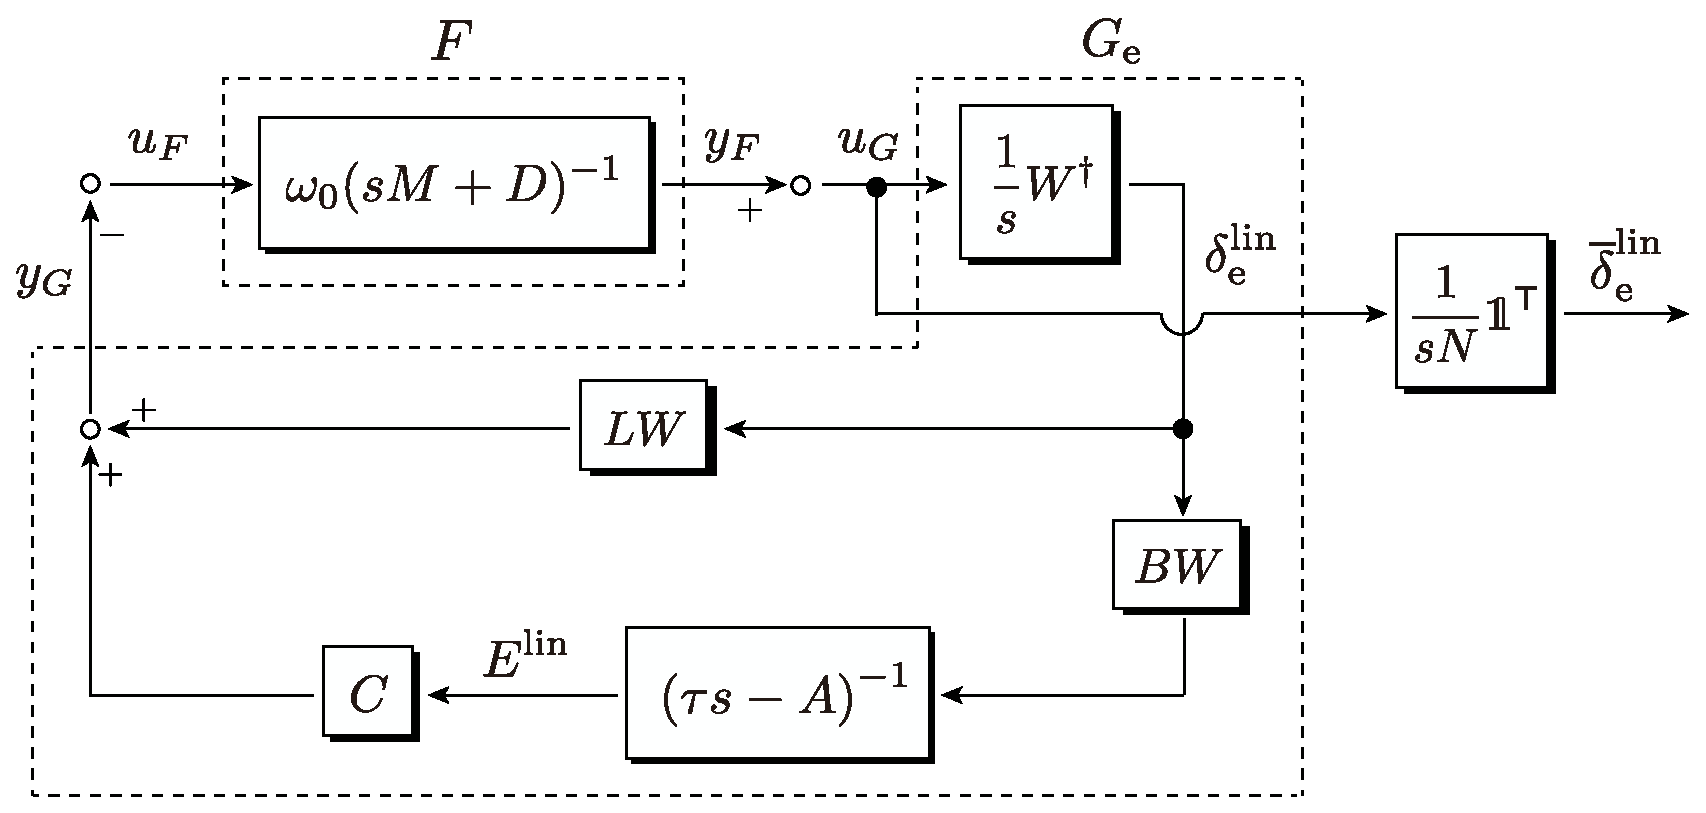
\includegraphics[width = .90\linewidth]{figs/FandGe2}
\medskip
\caption{\textbf{Basis-transformed approximate linear model}}
\label{fig:GandGe}
\medskip
\end{figure}


\smallskip
\subsubsection{Analysis of small signal stability based on passivity}

Below, we assume the passive power transmission conditions of definition \ref{def:passtrans} and show the passivity of $G_{\rm e}$ of Equation \ref{eq:Gsstrmin} using the same steps as the electrical system $G$ of Equation \ref{eq:Gss}.
To that end, we used the following expression:
\begin{align}\label{eq:Gecomdef}
G_{\rm e}: \simode{
\dot{x}_{G_{\rm e}} & = A_{G_{\rm e}} x_{G_{\rm e}} + B_{G_{\rm e}} u_G \\
y_G &= C_{G_{\rm e}} x_{G_{\rm e}}
}
\end{align}
$x_{G_{\rm e}}$ and ${\delta}^{\rm lin}_{\rm e}$ are vectors with $E^{\rm lin}$:
\[
A_{G_{\rm e}} := 
\mat{
0 & 0 \\
 \Omega^2 \hat{B} W  &  \Omega^2 \hat{A} 
},\quad
B_{G_{\rm e}} := 
\mat{
W^{\dagger} \\
0
},\quad
C_{G_{\rm e}} := 
\mat{
LW & -\hat{B}^{\sf T}
}
\]
A positive semi-definite matrix $P_{G_{\rm e}}$ is defined as:
\begin{align}\label{eq:defPGe}
P_{G_{\rm e}} := 
\mat{
W & 0 \\
0 & I
}^{\sf T}
\underbrace{
\mat{
L  &  - \hat{B}^{\sf T} \\
- \hat{B} & -\hat{A}
}
}_{P_G}
\mat{
W & 0 \\
0 & I
}
\end{align}
If $P_G$ of Equation \ref{eq:defPG} is positive semi-definite, $P_{G_{\rm e}}$ is also positive semi-definite.
\begin{align}\label{eq:Gelmi}
A^{\sf T}_{G_{\rm e}} P_{G_{\rm e}} + P_{G_{\rm e}} A_{G_{\rm e}} \preceq 
0
,\qquad
P_{G_{\rm e}} B_{G_{\rm e}} = C_{G_{\rm e}}^{\sf T}
\end{align}
At this time, because of the relationship of Equation \ref{eq:psudinv}, we can see that:
\[
\frac{
A^{\sf T}_{G_{\rm e}} P_{G_{\rm e}} + P_{G_{\rm e}} A_{G_{\rm e}}
}{2}
=
\mat{
\Omega \hat{B}W &0\\
0 & \Omega^{-1}
}^{\sf T}
\underbrace{
\mat{
-I & -\hat{A}_{\Omega} \\
-\hat{A}_{\Omega} & - \hat{A}_{\Omega}^2
}
}_{Y}
\mat{
\Omega \hat{B}W  &0\\
0 & \Omega^{-1}
}
\]
Therefore, the time derivative along the solution trajectory of $G_{\rm e}$ of the storage function:
\[
W_{G_{\rm e}}(x_{G_{\rm e}}):= \frac{1}{2}x_{G_{\rm e}}^{\sf T}P_{G_{\rm e}}x_{G_{\rm e}}
\]
can be evaluated as:
\begin{align}\label{eq:Glyapeq2}
\frac{d}{dt} W_{G_{\rm e}} \bigl( x_{G_{\rm e}} (t) \bigr)
 \leq 
y_G^{\sf T}(t) u_G(t)
\end{align}
In other words, $G_{\rm e}$ of Equation \ref{eq:Gsstrmin} is passive.
This inequality and inequality of Equation \ref{eq:Glyapeq} are equivalent, and the following is true for the values of two storage functions:
\[
W_{G} \bigl( x_{G} (t) \bigr) =
W_{G_{\rm e}} \bigl( x_{G_{\rm e}} (t) \bigr),\qquad
\forall t\geq 0
\]

By considering the observability of $G_{\rm e}$ shown by Equation \ref{eq:Geobs},
the following is true for the arbitrary initial value of the solution trajectory of the linear approximation model of Equation \ref{eq:lindynu0}:
\begin{align}\label{eq:allzero}
\lim_{t\rightarrow \infty} \Delta \omega^{\rm lin}(t)  =0,\qquad
\lim_{t\rightarrow \infty} \mat{
{\delta}^{\rm lin}_{\rm e}(t)   \\
E^{\rm lin}(t)  
}
 =0
\end{align}
Therefore, from the relationship of the change of basis of Equation \ref{eq:batrinv}, we can see that Equation \ref{eq:linmconv} holds for the arbitrary initial value.
In other words, the linear approximation model of Equation \ref{eq:lindynu0} is statically stable.
Also:
\[
c_0 = \lim_{t\rightarrow \infty}\overline{\delta}^{\rm lin}_{\rm e}(t)
\]
and state variables $\overline{\delta}^{\rm lin}_{\rm e}$ follow the differential equation of Equation \ref{eq:Gsstr}.

Let us theorize the above discussion in the following Theorem.

\begin{定理}[Small signal stability of the linear approximation model based on passivity]\label{thm:stasufcon}
For the arbitrary steady value $(\delta^{\star},E^{\star})$ that satisfies the passive power transmission conditions of definition \ref{def:passtrans}, the electrical subsystem $G$ of Equation \ref{eq:Gss} is passive.
For the arbitrary positive definite numbers $(M_i,D_i,\taudi )_{i \in \mathcal{I}_{\rm G}}$, the linear approximation model of Equation\ref{eq:lindynu0} is statically stable.
\end{定理}

As discussed in Theorem \ref{thm:stasufcon}, under the passive power transmission conditions, the linear approximation model is statically stable for combinations of all physical constants $(M_i,D_i,\taudi )_{i \in \mathcal{I}_{\rm G}}$.
Analysis based on passivity allows stability independent of model parameters.


%\begin{example}[基底変換による定態安定性の解析]
%\red{$W$の選び方に依らず等価な解析が可能であることを示す。}
%\end{example}

\subsection{Necessary conditions for the linear approximation model to be passive\advanced}\label{sec:nesconana}

\smallskip
\subsubsection{Passivity and positive realness}

Passivity of a linear system is mathematically equivalent to a property called positive realness of a transfer function.
In this Section, based on this equivalence, the necessity of the passive power transmission conditions of definition \ref{def:passtrans} is discussed from the viewpoint of the passivity of an electrical subsystem.

\begin{COLUMN}
\noindent \textbf{Transfer function}:
For a linear system:
\begin{align*}
\simode{
\dot{x}(t) & = Ax(t)+Bu(t) \\
y(t)&= Cx(t) + Du(t)
}
\end{align*}
its \textbf{transfer function} is defined as:
\[
Q(s):=C(sI-A)^{-1}B +D
\]
When the Laplace transform of the input $u(t)$ is $U(s)$, and the Laplace transform of the output $y(t)$ is $Y(s)$, there is a relationship, $Y(s)=Q(s)U(s)$, with a transfer function.
The input/output characteristics of a linear system are characterized by the transfer function.
\end{COLUMN}


The transfer function from the input $u_G$ to output $y_G$ of the electrical subsystem $G$ of Equation
\ref{eq:Gss} is:
\begin{align}\label{eq:trGs}
G(s) :=  - \frac{1}{s} 
\underbrace{
\left\{ -C \bigl( \taud s -A \bigr)^{-1} B - L \right\}
}_{H(s)}
\end{align}
Since unobservable state variables are not related to input/output characteristics, please note that the transfer function of $G_{\rm e}$ of Equation \ref{eq:Gsstrmin} is also equal to $G(s)$.
Below, let us consider a situation where the transfer function $H(s)$ of Equation \ref{eq:trGs} is stable.
The stability of the transfer function is defined as follows:

\begin{definition}[Stability of a transfer function]\label{def:trsta}
When the real part of all poles of the transfer function $Q(s)$ is negative, $Q(s)$ is called \textbf{stable}.
\end{definition}

The pole of a transfer function is the zero point of a denominator polynomial. The fact that $H(s)$ of Equation \ref{eq:trGs} is stable is equivalent to the
real part of all eigenvalues of the matrix $\taud^{-1}A$ being negative.

\textbf{Positive realness} of a transfer function is defined as follows:

\begin{definition}[Positive realness of a transfer function]\label{def:trpf}
For a square transfer function $Q(s)$, the following is defined:
\begin{align}\label{eq:defOm0}
\Omega_0 := \left\{
\omega_0 \in \mathbb{R}: 
\mbox{ 純虚数$\bm{j} \omega_0$が$Q(s)$の極である}
\right\}
\end{align}
When the following three conditions are satisfied, $Q(s)$ is called \textbf{positive real}.
\begin{itemize}
\item The real part of all poles of $Q(s)$ is nonpositive.
\item For all $\omega \in [0,\infty)\setminus \Omega_0$, $Q(\bm{j} \omega) + Q^{\sf T}(-\bm{j} \omega)$ is positive semi-definite.
\item When there are poles of a pure imaginary number, their multiplicity is 1, and the following is true for the remaining number: 
\begin{align*}
\lim_{s \rightarrow \bm{j} \omega_0} (s-\bm{j} \omega_0) Q(s) = \lim_{s\rightarrow \bm{j} \omega_0} \{ (s-\bm{j} \omega_0) Q(s)\}^{\sf *}\succeq 0
,\qquad
\forall \omega_0 \in \Omega_0
\end{align*}
\end{itemize}
\end{definition}


With definition \ref{def:trpf}, what is especially important is the first and second conditions.
The first condition shows the stability of a transfer function.
However, this includes the cases where the real part of the pole is 0.
The second condition is related to the positive definite nature of the Hermitian part when a transfer function is evaluated on an imaginary axis.

Specifically, when $Q(s)$ is a scalar; in other words, when input and output are both scalar, two conditions show that the real part of $Q(\bm{j}\omega)$ of all $\omega \in [0,\infty)\setminus \Omega_0$ is non-negative.
But please note that when $Q(s)$ is a matrix, it is usually:
\begin{align*}
Q(\bm{j} \omega) + Q^{\sf T}(-\bm{j} \omega) \neq 2 \real\left[ Q(\bm{j} \omega) \right]
\end{align*}
For $Q(s)$ with a real number coefficient, $Q^{\sf T}( -\bm{j} \omega)$ is equal to $\{Q(\bm{j} \omega)\}^*$.
The third condition is exceptions where $Q(s)$ has a pole of a pure imaginary number.
For example, as in $G(s)$ of Equation \ref{eq:trGs}, it is used to analyze the transfer functions with a pole at the origin.

\begin{COLUMN}
\noindent \textbf{Complex symmetric and complex skew-symmetric parts of a square matrix}:
Arbitrary square matrix $M$ can be broken down to
\[
M=\frac{M+M^*}{2}+\frac{M-M^*}{2}
\]
This $\tfrac{M+M^*}{2}$ is called the \textbf{Hermitian part} of $M$, while $\tfrac{M-M^*}{2}$ is called the \textbf{skew Hermitian part} of $M$.
\end{COLUMN}

In control systems engineering, it is known that the passivity in definition \ref{def:passivelin} and positive realness of definition \ref{def:trpf} are equivalent.
%\footnote{
%証明は\cite[Theorem 5.31]{antoulas2005approximation}や\cite[Theorem 3]{anderson1967system}などを参照されたい。
%また,\cite{kottenstette2010relationships}では,関連する一連の結果が細かく整理されている。
%\begin{補題*}
%安定かつ正方な伝達関数
%\[
%Q(s)=C(sI-A)^{-1}B + D
%\]
%を考える。
%ただし,$(A,B)$は可制御であり,$(C,A)$は可観測であるものとする。
%このとき,$Q(s)$が正実であるための必要十分条件は,
%ある正定対称行列$P$が存在して
%\begin{align*}%\label{eq:prlem}
%\mat{
%A^{\sf T}P+PA & PB-C^{\sf T} \\
%B^{\sf T} P -C & -(D+D^{\sf T})
%}\preceq 0
%\end{align*}
%が満たされることである。
%\end{補題*}
%}
%。
In the discussion in this Section, the necessary condition for $G(s)$ of Equation \ref{eq:trGs} to be positive real is that there is a positive definite matrix $P_{G_{\rm e}}$ that satisfies Equation \ref{eq:allzero} for $G_{\rm e}$ of Equation \ref{eq:Gecomdef}, which is a controllable and observable realization of state space.
This is equivalent to the passivity of $G_{\rm e}$ defined by the inequality of Equation \ref{eq:Glyapeq2}.
The fact that $P_{G_{\rm e}}$ of Equation \ref{eq:defPGe} is positive definite is shown by Schur complements related to $-\hat{A}$ and $-\hat{A}$:
\[
W^{\sf T} \left(L+\hat{B}^{\sf T} \hat{A}^{-1} \hat{B} \right) W
=  W^{\sf T} L_0 W
\]
being both positive definite.
However, since $L_0$ of Equation \ref{eq:defL0} satisfies \ref{eq:nescon} and the column vector of $W$ in Equation \ref{eq:batrinv} is orthogonal to $\mathds{1}$, $W^{\sf T} L_0 W$ is nonsingular.




\smallskip
\subsubsection{Necessary conditions for a transfer function of an electrical subsystem to be positive real}


As a mathematical preparation to derive necessary conditions, we introduce \textbf{negative imaginariness} of a transfer function, which is a similar concept to positive realness \cite{petersen2010feedback,xiong2010negative}.

\begin{definition}[Negative imaginariness of a transfer function]
\label{def:trni}
For a square transfer function $Q(s)$ without a pole at the origin, we define $\Omega_0$ of Equation \ref{eq:defOm0}.
When the following three conditions are satisfied, $Q(s)$ is called \textbf{negative imaginary}.
\begin{itemize}
\item The real part of all poles of $Q(s)$ is nonpositive.
\item For all $\omega \in (0,\infty)\setminus \Omega_0$, $\bm{j}\left\{Q(\bm{j} \omega) - Q^{\sf T}(-\bm{j} \omega) \right\}$ is positive semi-definite.
\item When there is a pole of a pure imaginary number, their multiplicity is 1, and the following holds for the remaining numbers:
\begin{align*}
\lim_{s \rightarrow \bm{j} \omega_0} (s-\bm{j} \omega_0) \bm{j} Q(s) = 
\lim_{s\rightarrow \bm{j} \omega_0} \{ (s-\bm{j} \omega_0) \bm{j} Q(s)\}^{\sf *}\succeq 0
,\quad
\forall \omega_0 \in \Omega_0
\end{align*}
\end{itemize}
\end{definition}

While the positive realness of definition \ref{def:trpf} was defined by the positive semi-definite nature related to the Hermitian part of a transfer function, the negative imaginariness of definition \ref{def:trni} is defined by the positive semi-definite nature of the skew Hermitian part of a
Specifically, when $Q(s)$ is scalar, the following is true:
\begin{align*}
\bm{j}\left\{Q(\bm{j} \omega) - Q^{\sf T}(-\bm{j} \omega) \right\}
= -2 \imag[Q(\bm{j} \omega)]
\end{align*}
thus, the second condition shows that for all $\omega \in (0,\infty)\setminus \Omega_0$, the imaginary part of $Q(\bm{j}\omega)$ is nonpositive.
Definition \ref{def:trni} includes a case where $Q(s)$ has a pole on an imaginary axis to contrast with definition \ref{def:trpf}, but in the following discussion, we need to only focus on the second condition to consider the negative imaginariness of a stable transfer function.
Similar to positive realness, the negative imaginariness of the transfer function is characterized as a possibility of matrix inequality. 
For more information, please refer to the supplemental title at the end of the Chapter \ref{lem:nilem}.
%\footnote{
%証明は\cite[Lemma 7]{xiong2010negative}などを参照されたい。
%\begin{補題*}
%安定かつ正方な伝達関数
%\[
%Q(s)=C(sI-A)^{-1}B + D
%\]
%を考える。
%ただし,$(A,B)$は可制御であり,$(C,A)$は可観測であるものとする。
%このとき,$Q(s)$が負虚であるための必要十分条件は,$D$が対称であり,かつ,
%ある対称正定行列$P$が存在して
%\begin{align*}
%A^{\sf T}P+PA \preceq 0
%,\qquad
%-PA^{-1}B = C^{\sf T}
%\end{align*}
%が満たされることである。
%\end{補題*}
%}
%。
%具体的には,式\ref{eq:siglin}の線形システム$\Sigma$の伝達関数が負虚であるための必要十分条件は,
%\[
%A^{\sf T} P  + PA \preceq 0 ,\qquad -PA^{-1}B = C^{\sf T}
%\]
%を満たす正定対称行列$P$が存在することである。
%ただし,式\ref{eq:siglin}の$\Sigma$は可制御かつ可観測であるものとする。




\begin{figure}[t]
  \centering
  {
  \begin{minipage}{0.49\linewidth}
    \centering
    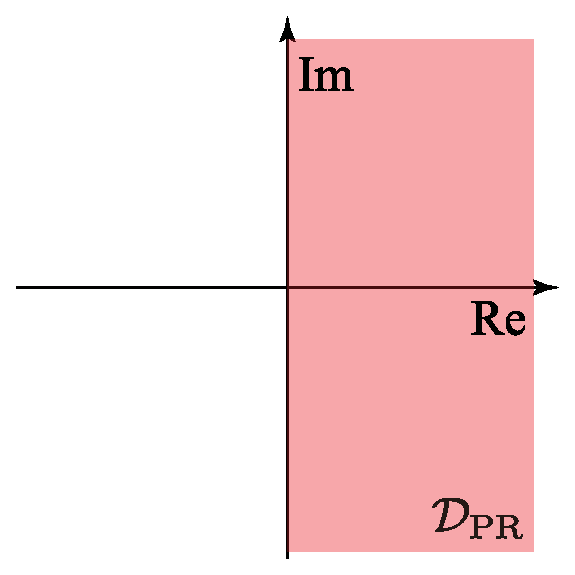
\includegraphics[width = .65\linewidth]{figs/PRdom}
    \subcaption{ $\mathcal{D}_{\rm PR}$ }
    \medskip
  \end{minipage}
  \begin{minipage}{0.49\linewidth}
    \centering
    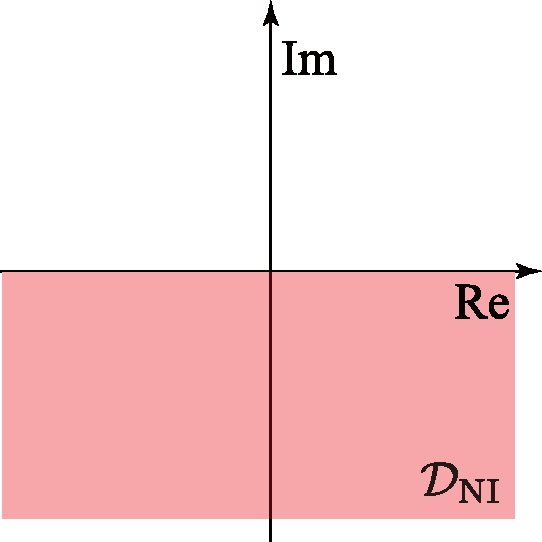
\includegraphics[width = .65\linewidth]{figs/NIdom}
    \subcaption{ $\mathcal{D}_{\rm NI}$ }
    \medskip
  \end{minipage}
  }
  \medskip
  \caption{\textbf{Positive realms and negative imaginary realms}}
  \label{fig:PRandNI}
\medskip
\end{figure}


\begin{COLUMN}
\noindent \textbf{Nyquist trajectory}:
When the trajectory related to $\omega \in \mathbb{R}$ of the frequency response function $Q(\bm{j} \omega)$ is plotted on a complex plane, it is called the \textbf{Nyquist curve}.
The Nyquist curve is often used for geometrical analysis related to the stability of a feedback system.
This analytical method is called the \textbf{Nyquist stability criterion}.
When $Q(s)$ is scalar, and the coefficient of the numerator polynomial and denominator polynomial is a real number, the trajectory of $Q(\bm{j} \omega)$ against negative $\omega$ is symmetrical to the trajectory and the real axis against positive $\omega$.
\end{COLUMN}

The relationship of positive realness and negative imaginariness is explained with Figure \ref{fig:PRandNI}.
If the transfer function $Q(s)$ is scalar, $Q(s)$ being positive real can be understood as the trajectory related to non-negative $\omega$ of the frequency response function $Q(\bm{j} \omega)$ is included in the range $\mathcal{D}_{\rm PR}$ shown in \ref{fig:PRandNI}(a).
\[
\mathcal{D}_{\rm PR} = \bm{j} \mathcal{D}_{\rm NI}
\]
and $-\tfrac{1}{\bm{j}}=\bm{j}$ for $G(s)$ and $H(s)$ of Equation \ref{eq:trGs}, the following is derived:
\[
G(\bm{j} \omega) \in \mathcal{D}_{\rm PR}, 
\quad \forall \omega >0
\qquad
\Longleftrightarrow
\qquad
H(\bm{j} \omega) \in \mathcal{D}_{\rm NI} ,
\quad \forall \omega >0
\]
Therefore, a negative imaginariness analysis of $H(s)$ is equivalent to a positive realness analysis of $G(s)$.
To be accurate, $G(\bm{j} \omega)$ and $H(\bm{j} \omega)$ are complex matrices; thus, $\mathcal{D}_{\rm PR}$ and $\mathcal{D}_{\rm NI}$ should be redefined with a set of positive semi-definite matrices.

Therefore, a negative imaginariness analysis of $H(s)$ is equivalent to a positive realness analysis of $G(s)$. Based on this fact, the passive power transmission conditions (ii) and (iii) are necessary conditions for $G(s)$ to be positive real.

\begin{定理}[Positive realness of the transfer function of an electrical subsystem]
\label{thm:EdynNI}
\red{Translated with DeepL}
For an arbitrary $(\delta^{\star},E^{\star})$ where the transfer function $H(s)$ of Equation \ref{eq:trGs} becomes stable, a condition necessary for $H(s)$ to be negative imaginary is that the passive power transmission condition (ii) of definition \ref{def:passtrans} holds.
In addition, a condition necessary for the transfer function $G(s)$ of Equation \ref{eq:trGs} to be positive real is that the passive power transmission conditions (ii) and (iii) hold.
\end{定理}

\begin{証明}
First, we show that for any $(\delta^{\star},E^{\star})$ for which $H(s)$ is stable, if $H(s)$ is negative imaginary, then the passive transmission condition (ii), i.e., the Equation \ref{eq:Gredcon}, holds.
Now
\[
\lim_{\omega \rightarrow \infty} \bm{j}
\left\{
H(\bm{j}\omega)-H^{\sf T}(-\bm{j}\omega)
\right\}
=\bm{j}
\left(
-L+L^{\sf T}
\right) \succeq 0
\]
Therefore, $L$ must be symmetric for $H(s)$ to be negative vacuity.
Thus, we have $K_{IJ}(\delta_{IJ}^{\star}) = K_{JI}(\delta_{JI}^{\star})$.
In other words
\[
G^{\rm red}_{ij} \sfsin \delta_{ij}^{\star} = 0 ,\qquad
\forall (i, j) \in \mathcal{I}_{\rm G} \times \mathcal{I}_{\rm G}
\]
This implies $\delta_{i}^{\star}\neq \delta_{j}^{\star}$ for $(i,j)$ where $G^{\rm red}_{ij}=0$.
Also, when $\delta_{i}^{\star}= \delta_{j}^{\star}$, continuity regarding parameter variation of eigenvalues for matrices with parameters implies that $\taud^{-1}A$ for $\delta^{\star}+\gamma e_i$ is There exists a sufficiently small $\gamma>0$ such that it is stable.
However, $e_i$ denotes a vector where only the $i$th $i$-element is 1 and the rest are 0.
Therefore, there exists a vector

\begin{align}\label{eq:Gij0t}
G^{\rm red}_{ij}=0, \qquad
\forall i\neq j
\end{align}
Furthermore, if $H(s)$ is negative imaginary, then
\[
\lim_{\omega \rightarrow 0} \bm{j}
\left\{
H(\bm{j}\omega)-H^{\sf T}(-\bm{j}\omega)
\right\}
=\bm{j}
\left(
-L_0+L_0^{\sf T}
\right) \succeq 0
\]
Therefore, $L_0$ in equation\ref{eq:defL0} must also be symmetric.
When the Equation\ref{eq:Gij0t} holds.
\[
C = \sfdiag \left(
2E_i^{\star} G^{\rm red}_{ii}
\right)  - \hat{B}^{\sf T}
\]
Note that $L_0$ is given by:
\[
L_0 = \underbrace{ L + \hat{B}^{\sf T} \hat{A}^{-1} \hat{B} }_{L_1}
-
\underbrace{ \sfdiag (
2 E_i^{\star} G^{\rm red}_{ii}
) \hat{A}^{-1} \hat{B}
}_{L_2}
\]
However, $\hat{A}$ is a symmetric matrix defined by the Equation \ref{eq:sysmats}.
On the other hand, for $L_2$ to be symmetric for any $E^{\star}$, it must have $G^{\rm red}_{ii}=0$ for all $i$.
From this, for any $(\delta^{\star},E^{\star})$ for which $H(s)$ is stable, if $H(s)$ is negative imaginary, then the expression \ref{eq:Gredcon} holds.

Next, we show that $H(s)$ is negative imaginary for any $(\delta^{\star},E^{\star})$ for which $H(s)$ is stable if the expression\ref{eq:Gredcon} holds.
This requires that $L$ is symmetric and:
\begin{align}\label{eq:cndQ}
\tilde{A}^{\sf T}P + P\tilde{A} \preceq 0
,\qquad
P\tilde{A}^{-1}\tilde{B}=C^{\sf T}
\end{align}
It is enough to show that there exists a positive definite matrix $P$ satisfying.
However, we need to show that there exists a positive definite matrix $P$ such that
\begin{align*}
\tilde{A}:= \taud^{-1}A
,\qquad
\tilde{B}:= \taud^{-1}B
\end{align*}
とする。
ここで,式\ref{eq:Gredcon}が成り立つならば
\begin{align*}
k_{ij}(\delta_{ij}^{\star}) =
k_{ji}(\delta_{ji}^{\star})
,\qquad
h_{ij}(\delta_{ij}^{\star}) = 
- h_{ji}(\delta_{ji}^{\star}),\qquad
h_{ii}(\delta_{ii}^{\star}) = 0
\end{align*}
Since $L$ is symmetric, it follows that $L$ is symmetric.
Also, since $H(s)$ is stable
\begin{align*}
\tilde{A} = 
\sfdiag \left( \frac{ \Xsi -  \Xti }{ \taudi } \right)
\hat{A}
\end{align*}
Since $\Xsi > \Xti$, $\hat{A}$ in Equation \ref{eq:sysmats} is negative definite.
Therefore, we can choose $-\hat{A}$ as the positive definite matrix $P$ satisfying Equation \ref{eq:cndQ}, which shows that $H(s)$ is negative-definite.


Next, we show the equivalence for $G(s)$.
Since $H(s)$ is stable, the only pole on the imaginary axis of $G(s)$ is the origin, and its degree of overlap is 1.
Therefore, $G(s)$ is
The necessary and sufficient condition for being positively real is:
\begin{align}\label{eq:Gpr}
G(\bm{j}\omega) + G^{\sf T}(-\bm{j}\omega) \succeq 0
,\qquad \forall \omega \in \mathbb{R}\setminus\{0\}
\end{align}
is valid, and the following can be established:
\begin{align}\label{eq:cndG0}
\lim_{s\rightarrow 0} s G(s) = \lim_{s\rightarrow 0} \{ s G(s)\}^{\sf T}\succeq 0
\end{align}
When the Equation \ref{eq:Gredcon} holds, then the Equation \ref{eq:Gpr} holds.
\begin{align}\label{eq:NIineq}
G(\bm{j}\omega) + G^{\sf T}(-\bm{j}\omega)
=
\frac{\bm{j}}{\omega} \left\{
H(\bm{j}\omega) - H^{\sf T}(-\bm{j}\omega)
\right\}
,\qquad \forall \omega \in \mathbb{R}\setminus\{0\}
\end{align}
It is shown from $H(s)$ that $H(s)$ is negative imaginary.
And,
\begin{align*}
\lim_{s\rightarrow 0} s G(s) =
L - C\tilde{A}^{-1}\tilde{B} = L - C A^{-1} B
\end{align*}
Therefore, the semi-positive definiteness of equation \ref{eq:cndG0} is equivalent to the passive transmission condition (iii), i.e., the condition of equation \ref{eq:pdsp}.
Note that when the passive transmission condition (ii) holds, $L$ is symmetric and:
\begin{align*}
C\tilde{A}^{-1}\tilde{B} = C P^{-1} C^{\sf T}
\end{align*}
is also symmetric, which also shows the symmetry of the expression \ref{eq:cndG0}.

Conversely, if the passive power transmission conditions (ii) or (iii) do not hold, then $G(s)$ is not positively real.
The latter is evident from the fact that the condition in equation \ref{eq:pdsp} is equal to the condition in equation \ref{eq:cndG0}.
Also, when the passive power transmission condition (ii) does not hold, since $H(s)$ is not negative vacuous, 
there exists a point $\omega_0\geq 0$ and a sufficiently small $\epsilon >0$ such that:
\begin{align*}
\lambda_{\rm min}\left[
\bm{j}
\left\{
H(\bm{j}(\omega_0 + \alpha )) - H^{\sf T}(-\bm{j}(\omega_0 + \alpha ))
\right\}
\right] < 0
,\qquad
\forall \alpha \in (0,\epsilon] 
\end{align*}
where $\lambda_{\rm min}$ denotes the smallest eigenvalue.
Thus, for all $\omega \in (\omega_0, \omega_0+\epsilon] $ that are not 0, the complex symmetric part of $G(\bm{j} \omega) $ is not semidefinite.
\end{証明}

\begin{figure}[t]
  \centering
  {
  \begin{minipage}{0.49\linewidth}
    \centering
    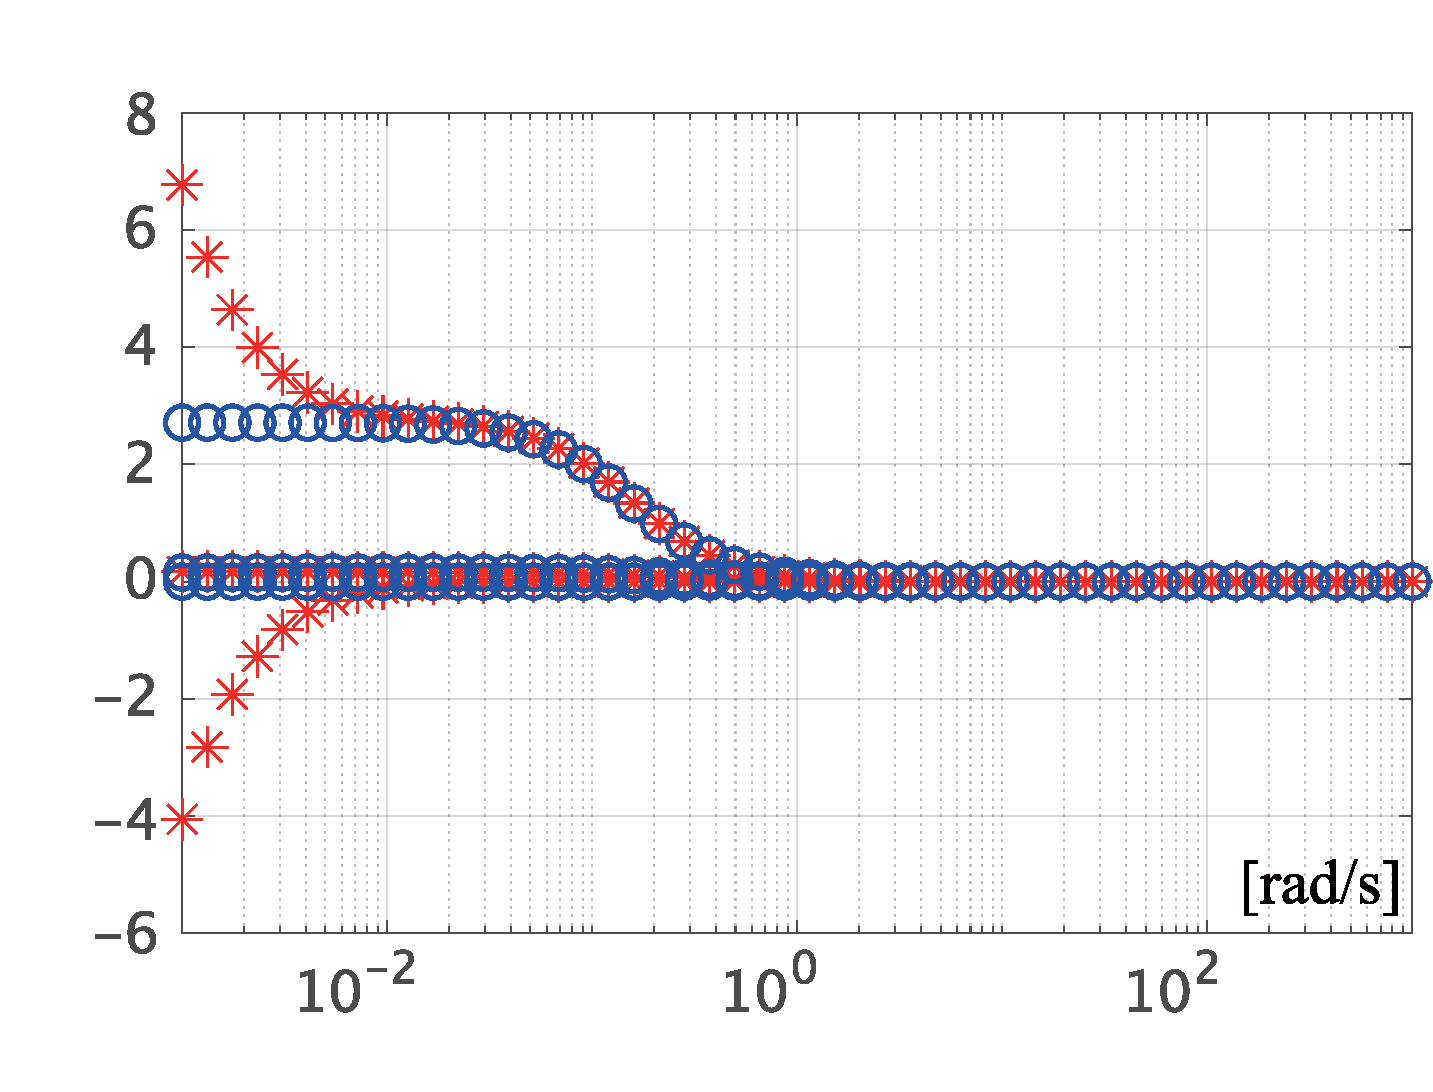
\includegraphics[width = 1.0\linewidth]{figs/eigG}
    \subcaption{ $\tfrac{G(\bm{j} \omega) + G^{\sf T}(-\bm{j} \omega)}{2} $の固有値}
    \medskip
  \end{minipage}
  \begin{minipage}{0.49\linewidth}
    \centering
    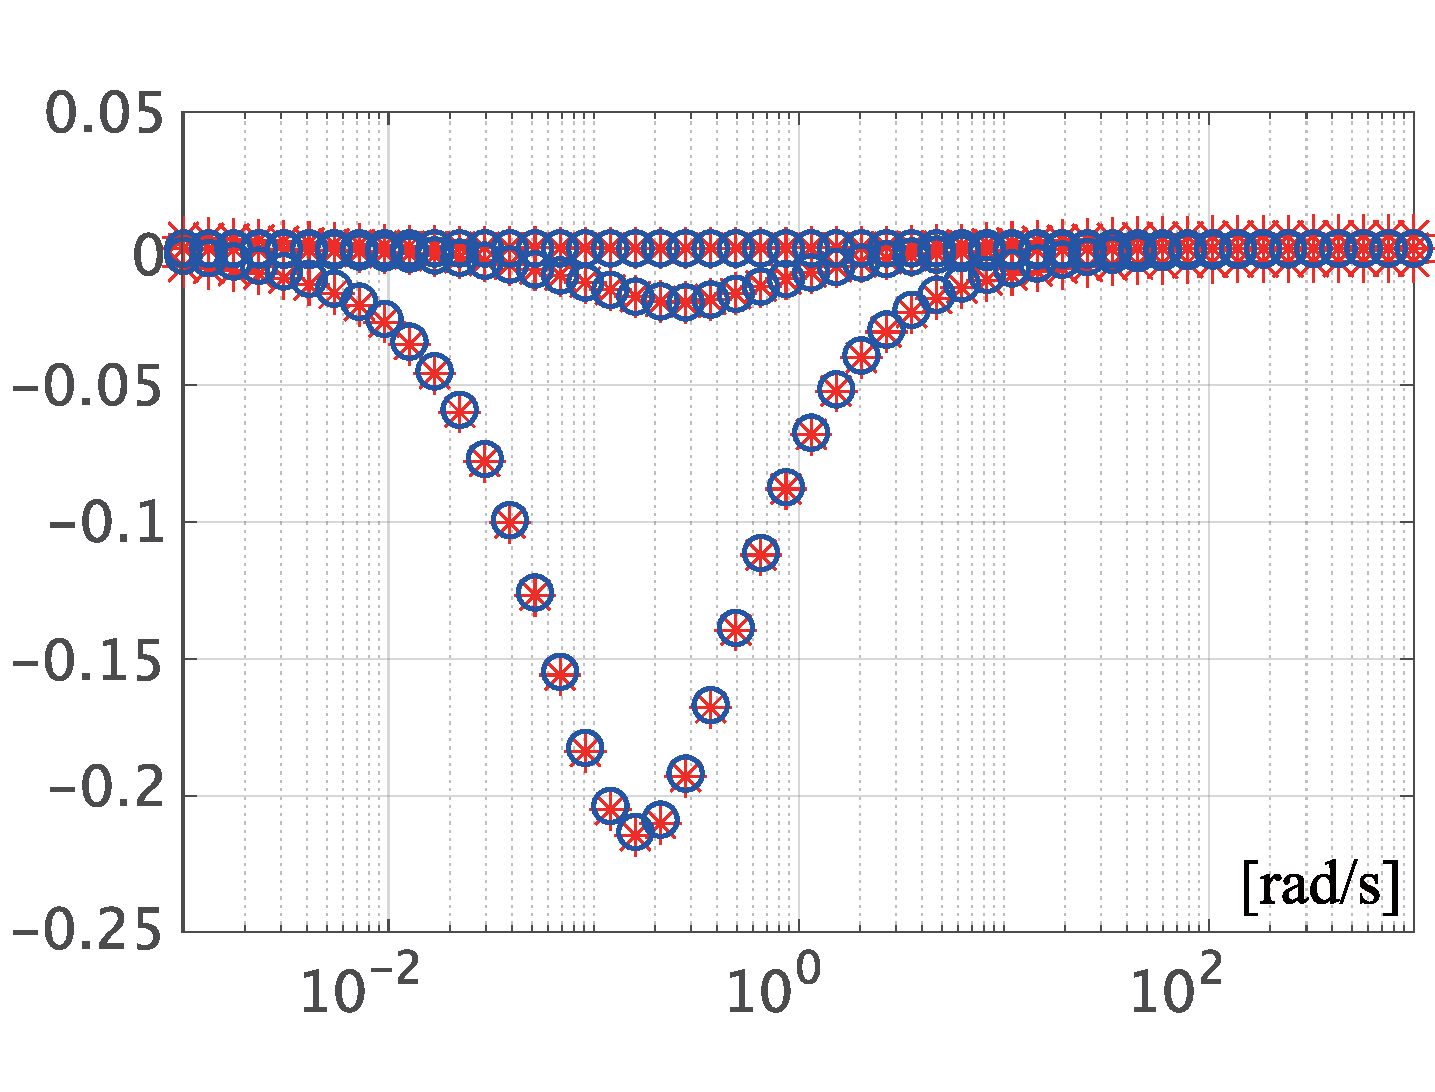
\includegraphics[width = 1.0\linewidth]{figs/eigH}
    \subcaption{ $\tfrac{H(\bm{j}\omega) - H^{\sf T}(-\bm{j}\omega)}{2\bm{j}}$の固有値}
    \medskip
  \end{minipage}
  }
  \medskip
  \caption{\textbf{$\bm{G(s)}$の正実性と$\bm{H(s)}$の負虚性}
  \\  \centering(Blue: passive transmission condition (ii) is satisfied, Red: not satisfied)}
  \label{fig:eigGH}
\medskip
\end{figure}


Let us confirm the result of Theorem \ref{thm:EdynNI} with an example.

\begin{example}[Transmission loss and positive realness of the transfer function of an electrical subsystemTransmission loss and positive realness of the transfer function of an electrical subsystem]
For the electrical power system model consisting of three generators discussed in the Example \ref{ex:linsyssim}, let us examine the positive realness of $G(s)$ and negative imaginariness of $H(s)$.
For comparison, we will calculate a case where the passive power transmission condition (ii) is satisfied, and when it is not satisfied.
Specifically, similar to the Example \ref{ex:energylin}, we set $\bm{Y}_0(0)$ and $\bm{Y}_0(1)$ as the admittance matrix $\bm{Y}$ of the power grid.
With the horizontal axis as frequency $\omega$, the eigenvalue of the Hermitian part of $G(\bm{j}\omega)$ is shown in Figure \ref{fig:eigGH}(a), while the imaginary part of the eigenvalue of the skew Hermitian part of $H(\bm{j}\omega)$ is shown in Figure \ref{fig:eigGH}(b).
The blue circle indicates when the passive power transmission condition (ii) is satisfied, while red indicates when it is not satisfied.
With this Figure, we can see that when the conductance of a transmission line is not 0, the Hermitian part of $G(\bm{j}\omega)$ is positive semi-definite in a low frequency band.
\end{example}

The significance of the passive power transmission condition (iii), which appeared as a condition for $P_G$ of Equation \ref{eq:defPG} to be positive semi-definite, can be explained as follows.
In the electrical subsystem $G$ of Equation \ref{eq:Gss}, let us look at the equation of state for the internal voltage: 
\begin{align*}
\taud
 \dot{E}^{\rm lin} = 
A E^{\rm lin} + B \delta^{\rm lin}
\end{align*}
With this differential equation, let us consider a limit at which the time constant $( \taudi )_{i \in \mathcal{I}_{\rm G}}$ asymptotically approaches 0.
This is equivalent to “a limit for which the time it takes for the internal voltage to reach a steady state is sufficiently shorter than the fluctuations in $\delta^{\rm lin}$”.
At this time, the following approximation holds:
\begin{align}\label{eq:spa}
E^{\rm lin}(t) \simeq  -A^{-1} B\delta^{\rm lin}(t)
,\qquad
\forall t\geq 0
\end{align}
If $A$ is not stable; in other words, if the passive power transmission condition (i) does not hold, state $E^{\rm lin}$ dissipates.
The method to approximate a differential equation with an algebraic equation using such a difference in the timescale of state variables is called \textbf{singular perturbation approximation} in control systems engineering.
Actually, the dynamic characteristics of the internal voltage often have smaller time constants compared to the dynamic characteristics of mechanical turbines.

If we assume Equation \ref{eq:spa} establishes an equation and substitutes as an output equation of Equation \ref{eq:Gss}, the following low-dimensional approximation of the electrical system is obtained:
\begin{align}\label{eq:Gsssp}
\hat{G}: \simode{
\dot{\hat{\delta}}^{\rm lin} & = u_G \\
y_G &= L_0 \hat{\delta}^{\rm lin}
}
\end{align}
To show that it is an approximation, we classified state variables as $\hat{\delta}^{\rm lin}$.
%また,内部電圧の近似的な値は
%\begin{align*}
%\hat{E}^{\rm lin}:=  -A^{-1} B \hat{\delta}^{\rm lin}
%\end{align*}
%として与えられる。
The entire linear approximation model of Equation \ref{eq:lindynu0} is approximated as a differential equation system where the second-order oscillator is combined by this singular perturbation approximation:
\begin{align}\label{eq:spamodel}
M \ddot{\hat{\delta}}^{\rm lin}
+ D \dot{\hat{\delta}}^{\rm lin}
+\omega_0 L_0 \hat{\delta}^{\rm lin}=0
\end{align}
This result shows that the passive power transmission condition (iii) shows the “positive semi-definite nature of a spring constant matrix” when the time constant is small.
It can be interpreted as equivalent to a dynamic spring constant of the electrical subsystem $G$ of Equation \ref{eq:Gss}.

\begin{figure}[t]
  \centering
  {
  \begin{minipage}{0.49\linewidth}
    \centering
    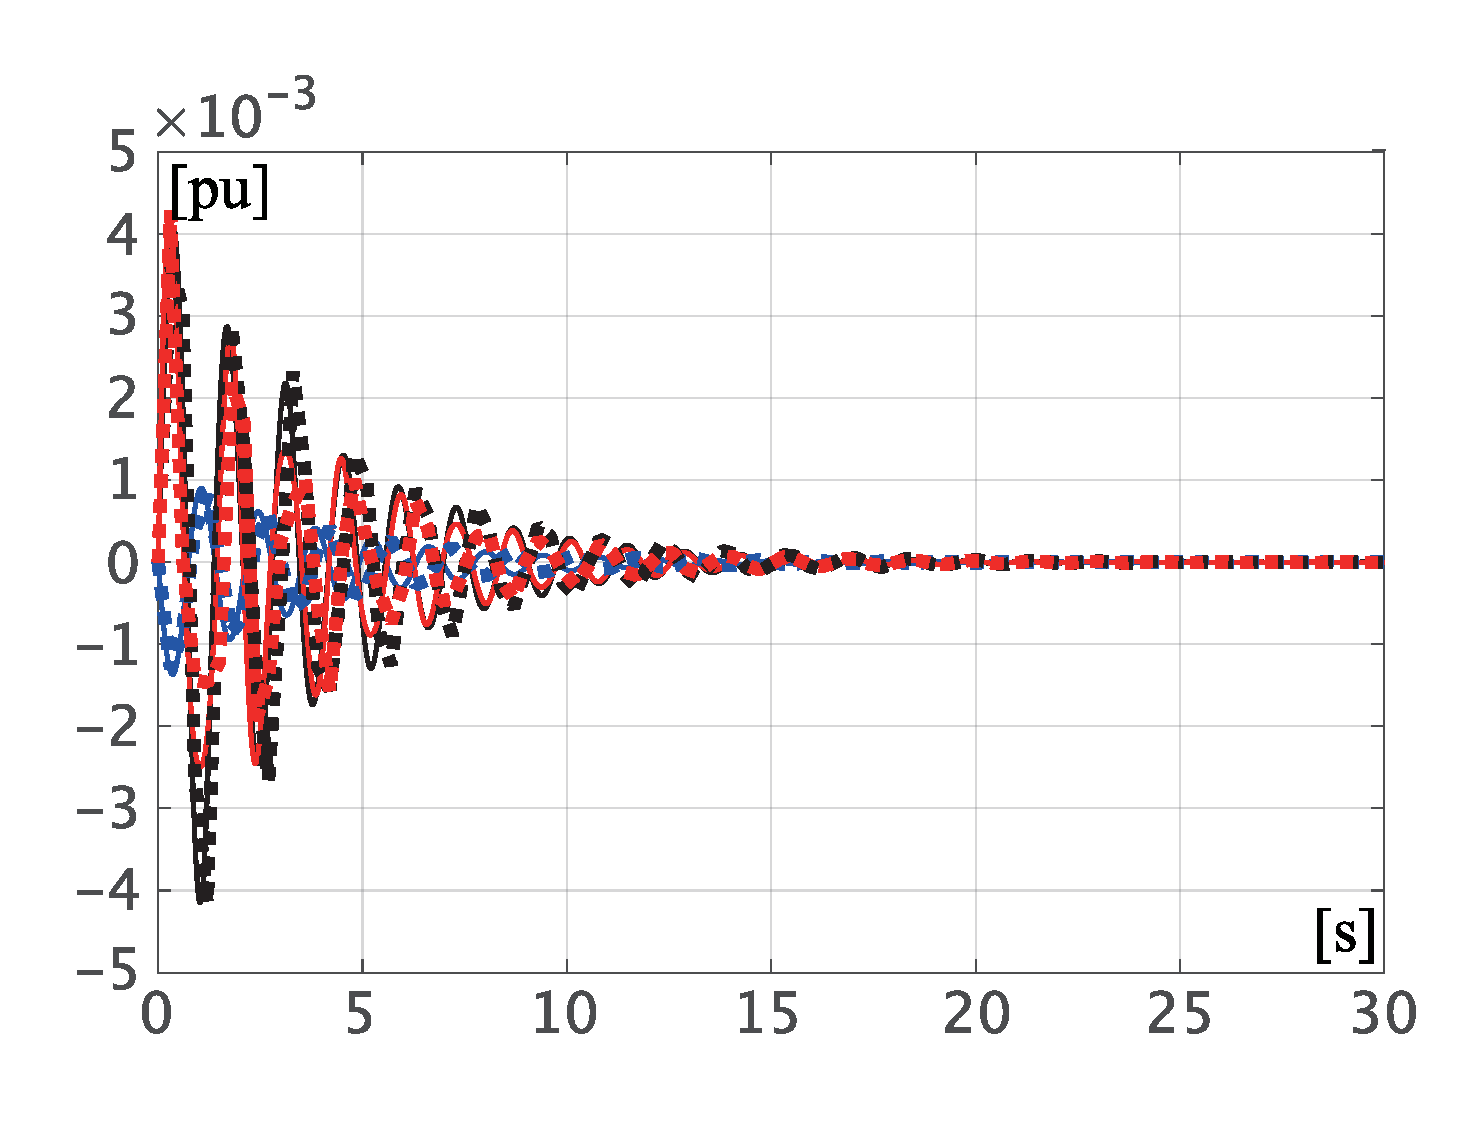
\includegraphics[width = 1.0\linewidth]{figs/Domegaspa}
    \subcaption{ Solid line: $\Delta \omega^{\rm lin}$, Dotted line: $\Delta \hat{\omega}^{\rm lin}$ }
    \medskip
  \end{minipage}
  \begin{minipage}{0.49\linewidth}
    \centering
    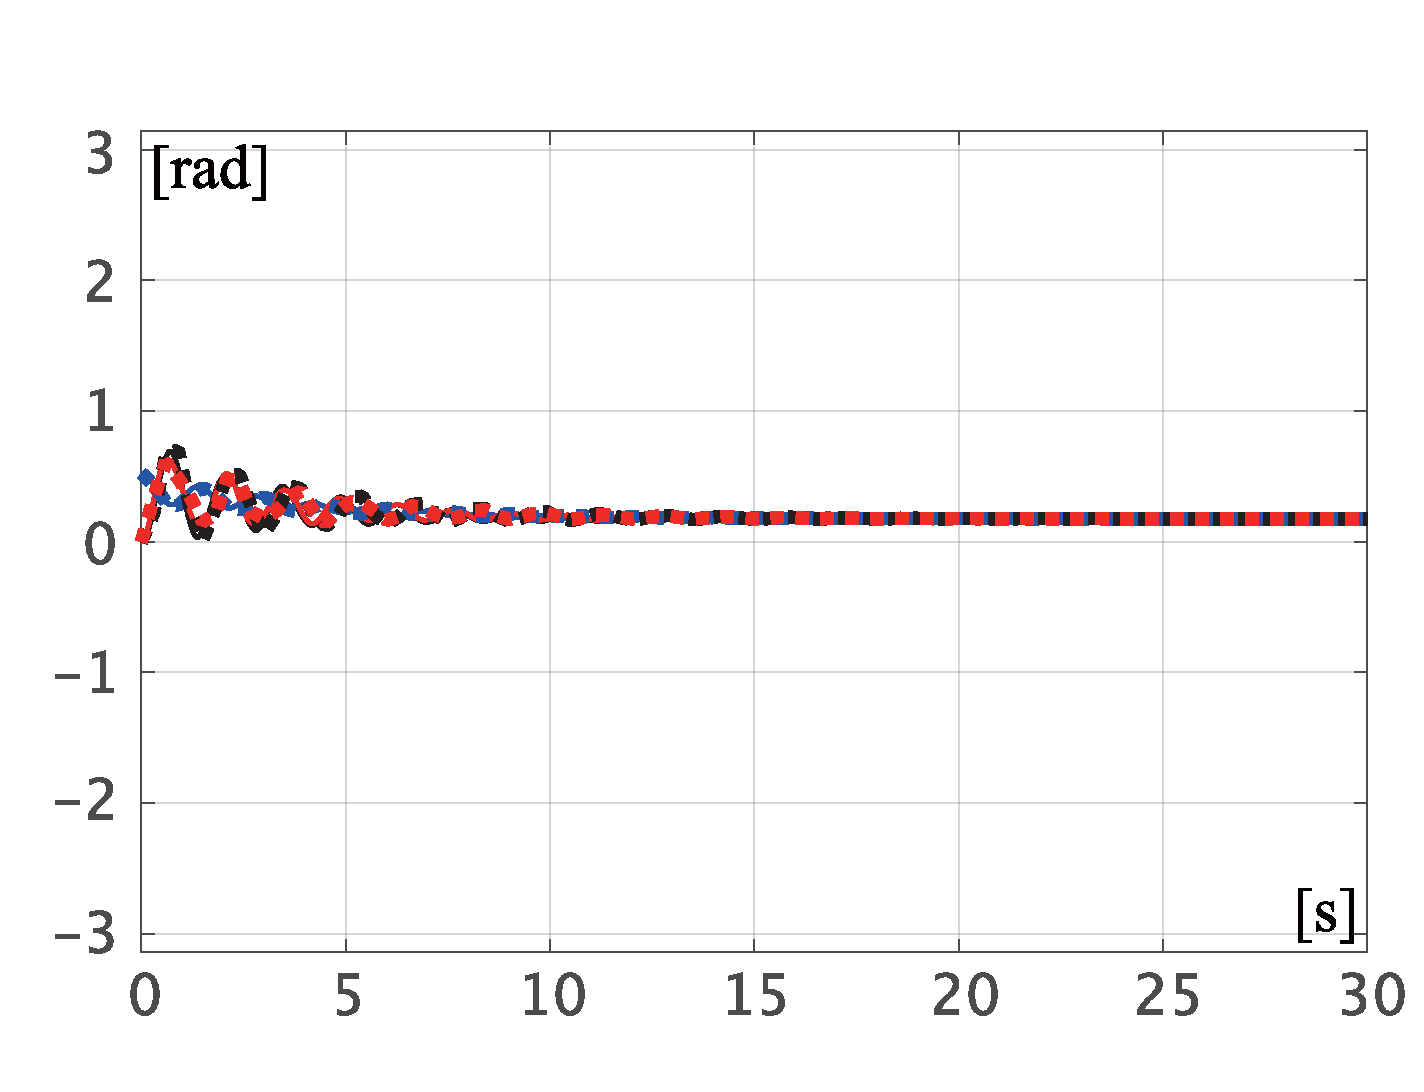
\includegraphics[width = 1.0\linewidth]{figs/deltaspa}
    \subcaption{ Solid line:$\delta^{\rm lin}$, Dotted line:${\hat{\delta}}^{\rm lin}$ }
    \medskip
  \end{minipage}
 \begin{minipage}{0.49\linewidth}
    \centering
    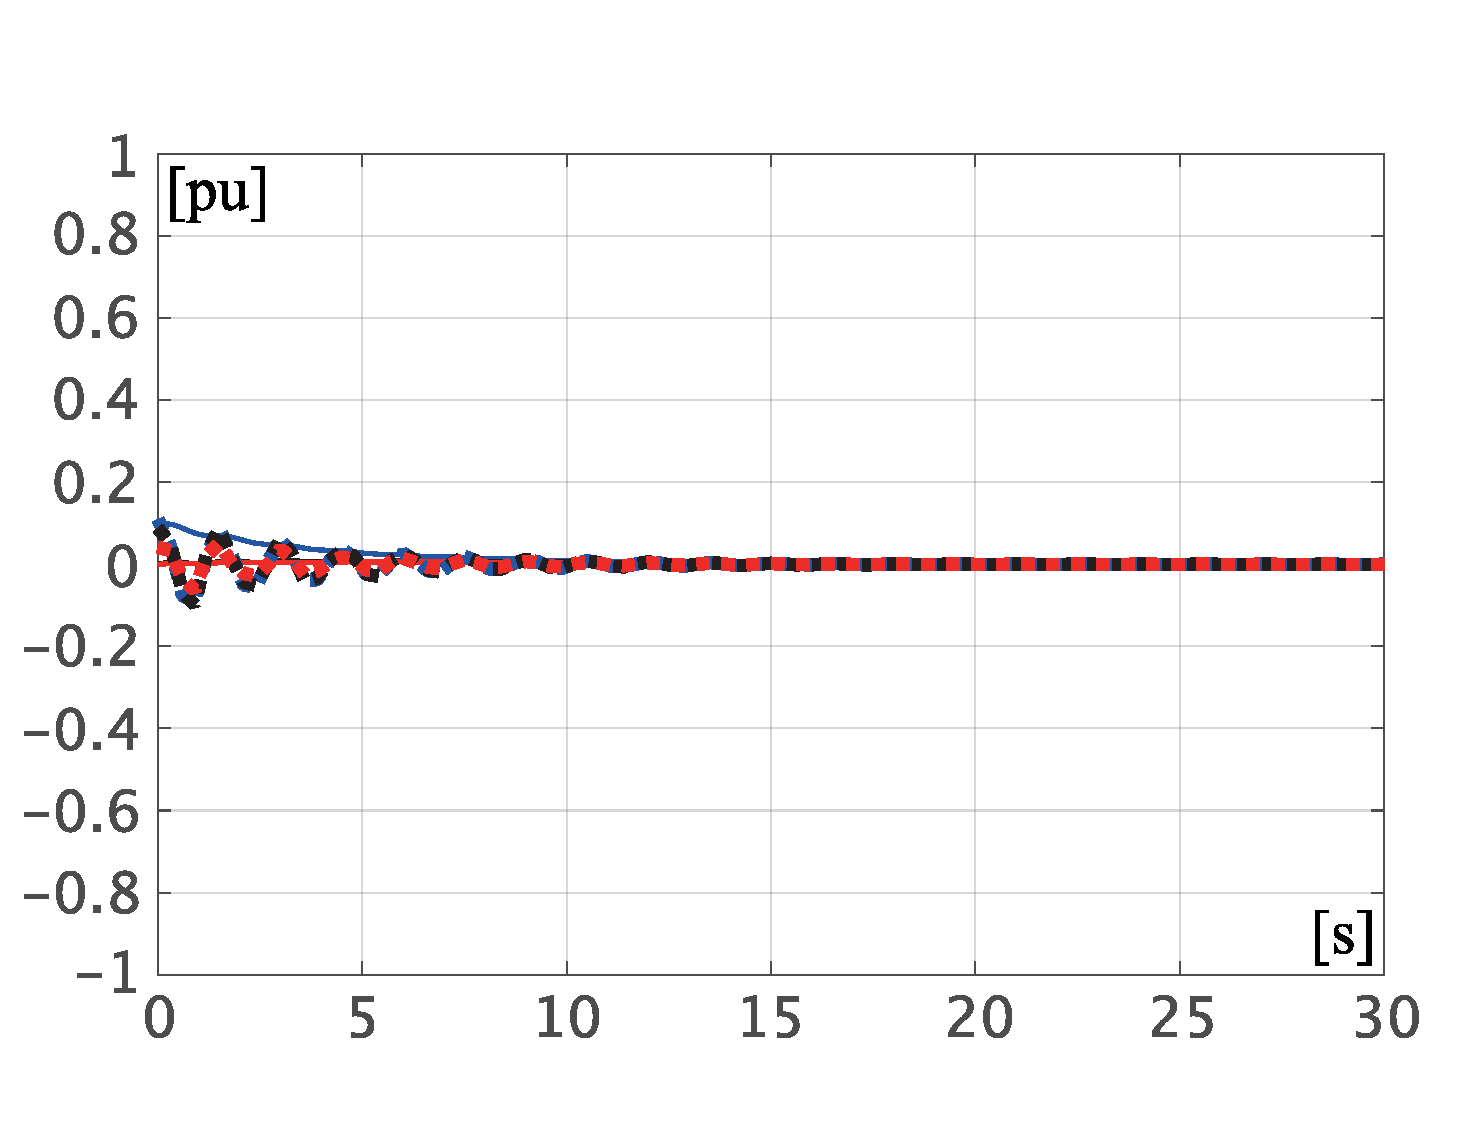
\includegraphics[width = 1.0\linewidth]{figs/Espa}
    \subcaption{ Solid line:$E^{\rm lin}$, Dotted line:$\hat{E}^{\rm lin}$ }
    \medskip
  \end{minipage}
  \begin{minipage}{0.49\linewidth}
    \centering
    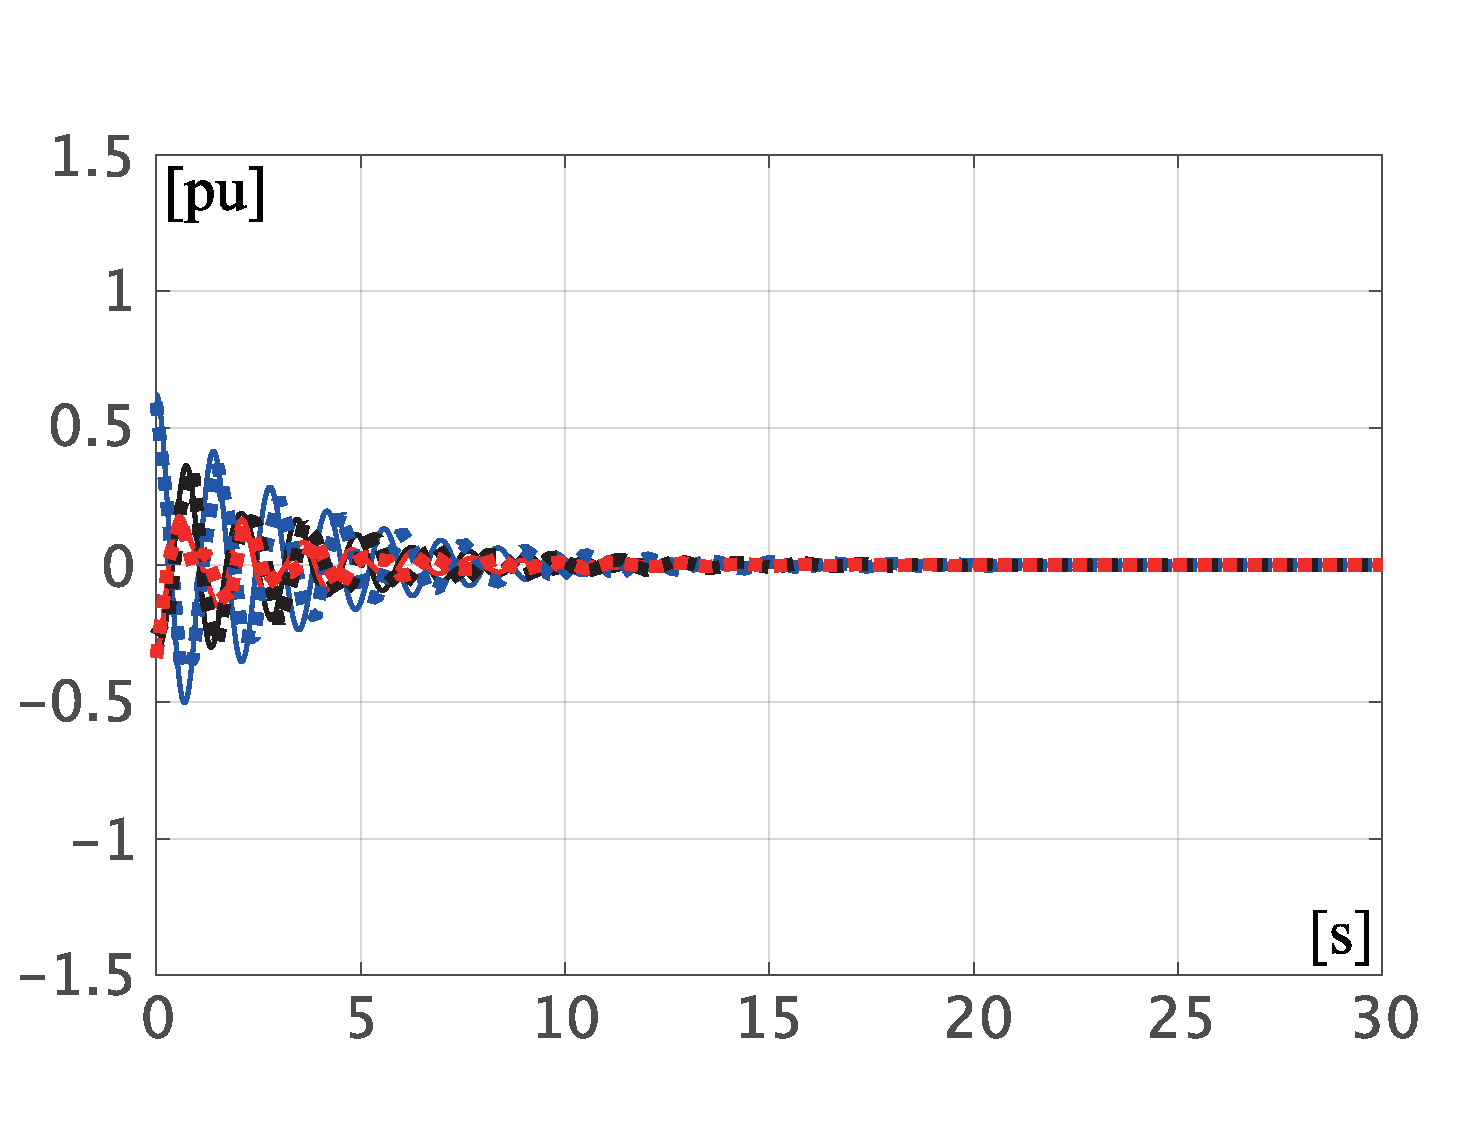
\includegraphics[width = 1.0\linewidth]{figs/Pspa}
    \subcaption{ Solid line:$P^{\rm lin}$, Dotted line:$\hat{P}^{\rm lin}$ }
    \medskip
  \end{minipage}
  }
  \medskip
  \caption{\textbf{Time response when low-dimensional approximation is applied}
  \\  \centering(Blue: Generator 1, Black: Generator 2, Red: Generator 3)}
  \label{fig:timeexsp}
\medskip
\end{figure}


%\begin{figure}[t]
%  \centering
%  {
%  \begin{minipage}{0.49\linewidth}
%    \centering
%    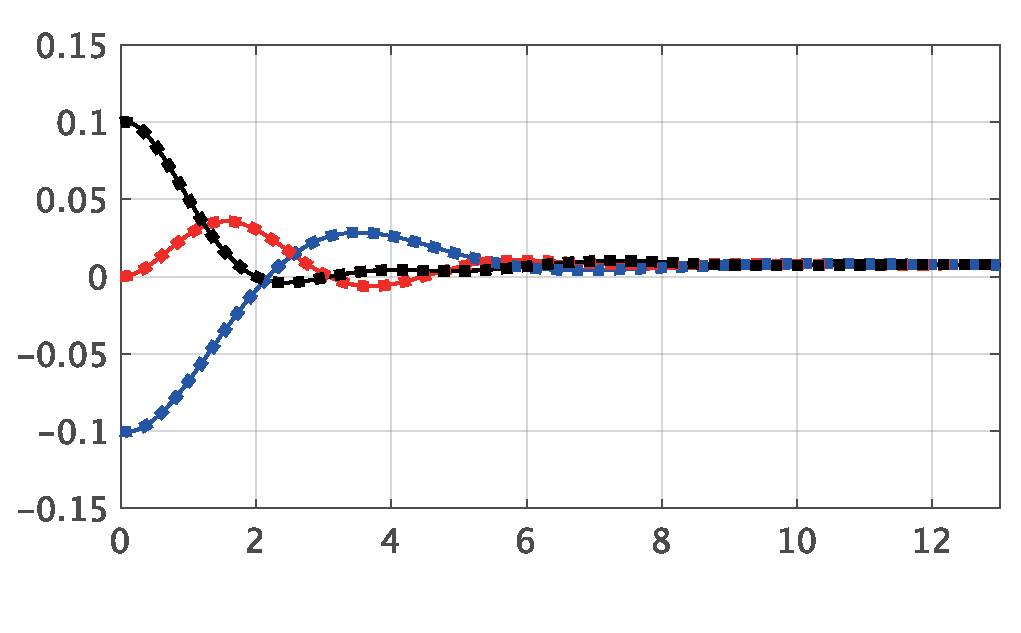
\includegraphics[width = 1.0\linewidth]{figs/deltasp}
%    \subcaption{ $\hat{\delta}^{\rm lin}$ }
%    \medskip
%  \end{minipage}
%  \begin{minipage}{0.49\linewidth}
%    \centering
%    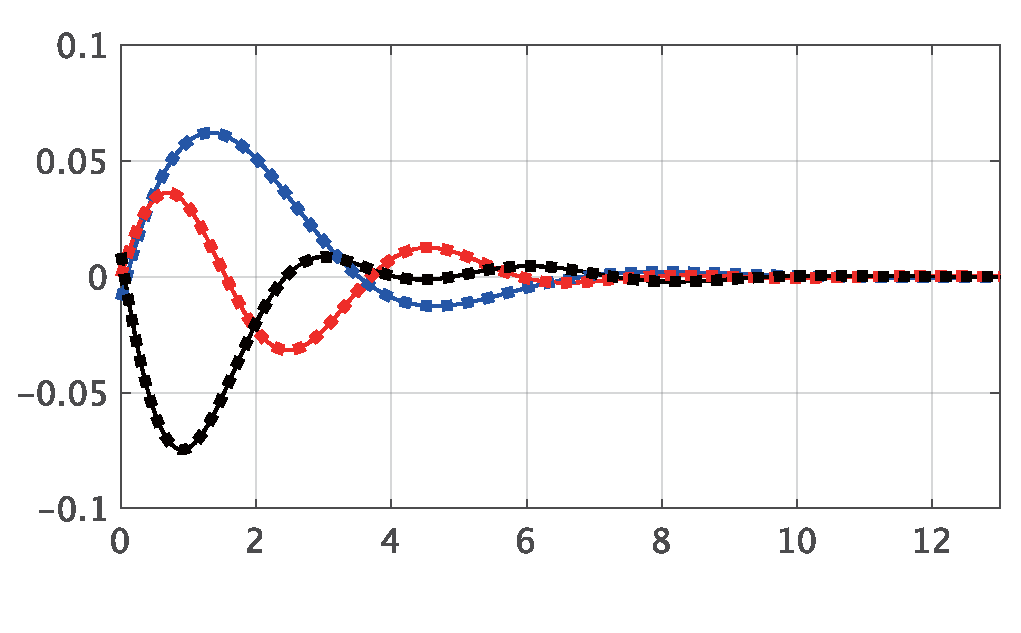
\includegraphics[width = 1.0\linewidth]{figs/omegasp}
%    \subcaption{ $\Delta \hat{\omega}^{\rm lin}$ }
%    \medskip
%  \end{minipage}
%%  \begin{minipage}{0.32\linewidth}
%    \centering
%    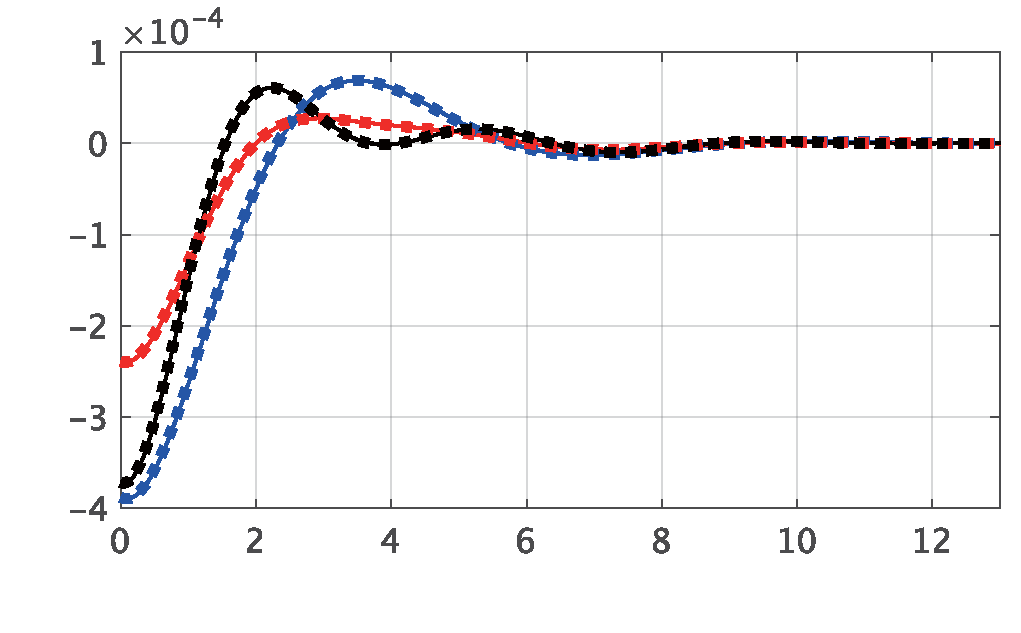
\includegraphics[width = .49\linewidth]{figs/Esp}
%    \subcaption{ $\hat{E}^{\rm lin}$ }
%%  \end{minipage}
%  }
%  \medskip
%  \caption{\textbf{特異摂動近似モデルの初期値応答}}
%  \label{fig:timeexsp}
%\medskip
%\end{figure}


\begin{example}[Singular perturbation approximation of a linear approximation model]
As a reference, Figure \ref{fig:timeexsp} shows the time response of a second-order oscillator system of Equation \ref{eq:spamodel} to the linear approximation model discussed in the Example \ref{ex:linsyssim}.
The solid line is the response of the original linear approximation model, while the dashed line is the response of a second-order oscillator system after applying the singular perturbation approximation.
Also:
\[
\Delta \hat{\omega}^{\rm lin}:=\omega_0^{-1} \dot{\hat{\delta}}^{\rm lin},\qquad
\hat{E}^{\rm lin}:=-A^{-1}B\hat{\delta}^{\rm lin},\qquad
\hat{P}^{\rm lin}:= L \hat{\delta}^{\rm lin} + C \hat{E}^{\rm lin}
\]
The initial value of the linear approximation model is given as follows in response to Equation \ref{eq:linmini}:
\[
\hat{\delta}^{\rm lin}(0)
 =
\mat{
\tfrac{\pi}{6} \\
0 \\
0
},\qquad
\Delta \hat{\omega}^{\rm lin}(0)
 =
\mat{
0 \\
0 \\
0
}
\]
Figure \ref{fig:timeexsp} shows that the time response of both is largely consistent with the peak value of the oscillations and attenuation rate.
\end{example}

\subsection{Necessary conditions for the linear approximation model to be statically stable\advanced}\label{sec:nesconsta}

Below, we discuss the necessity of the passive power transmission condition (iii) from the viewpoint of small signal stability of the linear approximation model of Equation \ref{eq:lindynu0}.
Specifically, it shows that the passive power transmission condition (iii) is a necessary condition for the linear approximation model to be statically stable regardless of the physical constants of generators.
As shown in the discussions of Section \ref{sec:nesconana}, the passive power transmission condition (i) is a necessary condition for the linear approximation model to not be unstable for the time constant $(\taudi)_{i \in \mathcal{I}_{\rm G}}$ at a sufficiently small limit.
When the matrix $A$ is not stable, this can be confirmed from the dissipation of the internal voltage since the singular perturbation approximation of Equation \ref{eq:spa} cannot be applied. 

When the passive power transmission condition (ii) does not hold, since $L_0$ is usually not symmetrical, we consider generalization of the passive power transmission condition (iii) so that it can be applied to unsymmetrical $L_0$:
\begin{align}\label{eq:eigreal}
\bm{\Lambda}(L_0)\subseteq [0,\infty)
\end{align}
However, $\bm{\Lambda}(L_0)$ shows a set of eigenvalues of $L_0$.
The conditions of Equation \ref{eq:eigreal} show that all eigenvalues of $L_0$ are “non-negative real numbers”.
Below, we call this generalized condition the passive power transmission condition (iii) $'$ of definition \ref{def:passtrans}.
When $L_0$ is symmetrical, the passive power transmission conditions (iii) and (iii)$'$ are equivalent.
The following lemma is presented.

\begin{補題}[Necessary condition for the small signal stability of a second-order oscillator system]\label{thm:2ndsys}
Let us consider a second-order oscillator system of Equation \ref{eq:spamodel}.
For an arbitrary initial value and arbitrary positive definite number $(M_i,D_i)_{i \in \mathcal{I}_{\rm G}}$, a condition necessary for a certain constant $c_0$ to exist and the following to hold:
\begin{align}\label{eq:delhat0}
\lim_{t\rightarrow \infty} \hat{\delta}^{\rm lin}(t)= c_0 \mathds{1}
\end{align}
is that the passive power transmission condition (iii)$'$ holds.
\end{補題}

\begin{証明}
\red{Translated with DeepL}
If the passive transmission condition (iii)$'$ does not hold, then there exists a certain positive constant $(M_i,D_i)_{i \in \mathcal{I}_{\rm G}}$ such that the Equation \ref{eq:delhat0}.
For this purpose, the following two cases will be discussed.
\begin{itemize}
\item[(a)] Among the eigenvalues of $L_0$, there exist eigenvalues whose real part is negative or pure imaginary.
\item[(b)] There exist eigenvalues of $L_0$ whose real part is positive and whose imaginary part is nonzero.
\end{itemize}
First, let's consider the case (a).
In the following, we choose constant matrices as $M=\omega_0 I$ and $D=\omega_0 d I$.
In this case, the eigen equation of the equation \ref{eq:spamodel} are
\begin{align*}
\mat{
0 & I \\
-L_0 & -d I
}
\mat{v\\w}
=
\lambda \mat{v\\w}
\end{align*}
If $ w $ is eliminated from this equation by substitution, the following is obtained:
\begin{align*}
\left(\lambda^2 I +d \lambda I + L_0
\right) v =0
\end{align*}
This eigenvalue is an eigenvector with $ v $ of $ L_0 $ and for that eigenvalue $ \kappa $, and therefore the following is true.
\begin{align}\label{eq:lamsq}
\lambda^2 + d\lambda +\kappa =0
\qquad
\Longleftrightarrow
\qquad
\lambda = \frac{-d \pm \sqrt{d^2-4\kappa} }{2}
\end{align}
Therefore, in the case of (a), it is sufficient to show that the real part of $ \sqrt{d^2--4\kappa} $ is larger than $ d $.
In general, for any complex number $ \bm{z} $
\begin{align*}
\real[\bm{z}] = \sqrt{ \real[\bm{z}^2 ] + (\imag[\bm{z}])^2 }
\end{align*}
Since it can be expressed as $ \bm{z} = \sqrt{d^2--4\kappa} $, the following result can be obtained:
\begin{align*}
\real \Bigl[
\sqrt{d^2 - 4\kappa }
\Bigr]
=\sqrt{
d^2 - 4 \real[\kappa]
+
(\imag[ \bm{z} ])^2
}
\end{align*}
This value is in case (a), that is, when the real part of $ \kappa $ is negative, or the real part of $ \kappa $ is 0 and the imaginary part of $ \kappa $ is non-zero.Must be greater than $ d $.
Therefore, the secondary oscillator system of the equation \ref{eq: spamodel} is unstable.

Next, consider the case of (b).
In the following, it is shown that there exists a positive constant $ d $ such that the eigenvalue $ \lambda $ of the expression \ref{eq: lamsq} is a pure imaginary number.
When $ L_0 $ in the execution column has a complex eigenvalue, there is always something with a negative imaginary part.
The eigenvalue is expressed as $ \kappa = \alpha + \beta \bm {j} $ using $ \alpha> 0 $ and $ \beta <0 $.
For this $ \kappa $, there exists $ \omega \neq 0 $ and $ d> 0 $ that satisfy: 
\[
-d + \sqrt{d^2-4\kappa}  = \omega \bm{j}
\]
If you transfer $ -d $ on the left side and square both sides:
\[
-4 (\alpha + \beta \bm{j}) = 2d \omega \bm{j} -\omega^2
\]
This equation is satisfied by choosing $ \omega = 2 \sqrt {\alpha} $, $ d =-\tfrac {\beta} {\sqrt {\alpha}} $.
Therefore, since the secondary oscillator system has a steady-state vibration solution, the equation \ref{eq: delhat0} does not hold.
\end{証明}


Lemma \ref{thm:2ndsys} shows that, for a limit where the time constant of the internal voltage is sufficiently small, the passive power transmission condition (iii)$'$ is a necessary condition for the linear approximation model to be statically stable against the arbitrary physical constants of generators.
Furthermore, with Theorem \ref{thm:stasufcon}, when the passive power transmission conditions (i)--(iii) hold, the linear approximation model is stable against arbitrary physical constants.
Based on these facts, the conclusion of this Section is summarized in the following Theorem.


\begin{定理}[Small signal stability of the linear approximation model]\label{thm:sync}
For an arbitrary positive definite number $(M_i,D_i,\taudi)_{i \in \mathcal{I}_{\rm G}}$, a necessary condition for the linear approximation model of Equation \ref{eq:lindynu0} to be statically stable is that the passive power transmission conditions (i) and (iii)$'$ of definition \ref{def:passtrans} hold.
Specifically, when the passive power transmission condition (ii) holds, the above-mentioned necessary condition for the small signal stability is that the passive power transmission conditions (i) and (iii)$'$ hold.
\end{定理}

We present an analytical example of the small signal stability of the linear approximate model using Theorem \ref{thm:sync}.

\begin{example}[Small signal stability analysis based on the passive power transmission conditions]\label{ex:linthm}
Using Theorem \ref{thm:sync}, let us analyze the small signal stability of the linear approximation model consisting of three generators discussed in the Example \ref{ex:linsyssim}.
The physical constants of generators are set to the same value as Example \ref{ex:linsyssim}.
Since the passive power transmission condition (i) was satisfied for all parameters, we also plotted the range or parameters where the passive power transmission condition (iii) $'$ is not satisfied in Figure \ref{fig:stacheckX}.
When the eigenvalue of $L_0$ of Equation \ref{eq:defL0} includes those where the real part is negative, it is shown in red.
When the eigenvalue of complex numbers is included, it is shown with purple.
This shows when the passive power transmission condition (ii) holds for the range on the horizontal axis where $\theta_2$ is 0.

Theorem \ref{thm:sync} shows that the ranges shown with red and purple are “dangerous parameter ranges where the linear approximation model is always unstable with some physical constant settings”.
When the passive power transmission condition (ii) holds; in other words, for parameters on the horizontal axis where $\theta_2$ is 0, as long as $\theta_1$ is set to a value that is not red, the linear approximation model has a small signal stability regardless of the value of these constants.

What we need to pay attention to in the result of Figure \ref{fig:stacheckX} is that the parameter range shown in red accurately captures some or all of the boundaries with the blue parameter range, where static stability is achieved with the above-described physical constants.
The necessity of the passive power transmission condition (iii)$'$ shown with Theorem \ref{thm:sync} means that there is at least one setting of physical constants for generators where the linear approximation model is unstable.
Therefore, for the specific constants set in the Example \ref{ex:linsyssim}, the parameter ranges for static stability cannot always be captured accurately.
On the other hand, the fact that the some boundaries of the blue range are accurately captured indicates that when the real part of $L_0$ has negative eigenvalues, in many cases, the linear approximation model is unstable.

In the cases of (a) and (b), there is no blue range.
In other words, for the searched parameters, the eigenvalue of $L_0$ is a real number.
Generally, as long as $\theta_2$ is not 0, $L_0$ is a non-symmetrical matrix; thus, it is unclear whether only $L_0$ has a real eigenvalue.
On the other hand, in (c) and (d) where the admittance matrix is multiplied by $\tfrac{1}{100}$, if $\theta_1$ and $\theta_2$ are relatively large, $L_0$ has a complex eigenvalue.
However, in a realistic setting, it has been confirmed that $L_0$ often only has real eigenvalues.
%なお,アドミタンス行列はインピーダンス行列と逆行列の関係にあるため,アドミタンス行列の大きさが小さいことは,送電線のレジスタンスやリアクタンスが大きいことを表している。
\end{example}


\begin{figure}[t!]
  \centering
  {
  \begin{minipage}{0.49\linewidth}
    \centering
    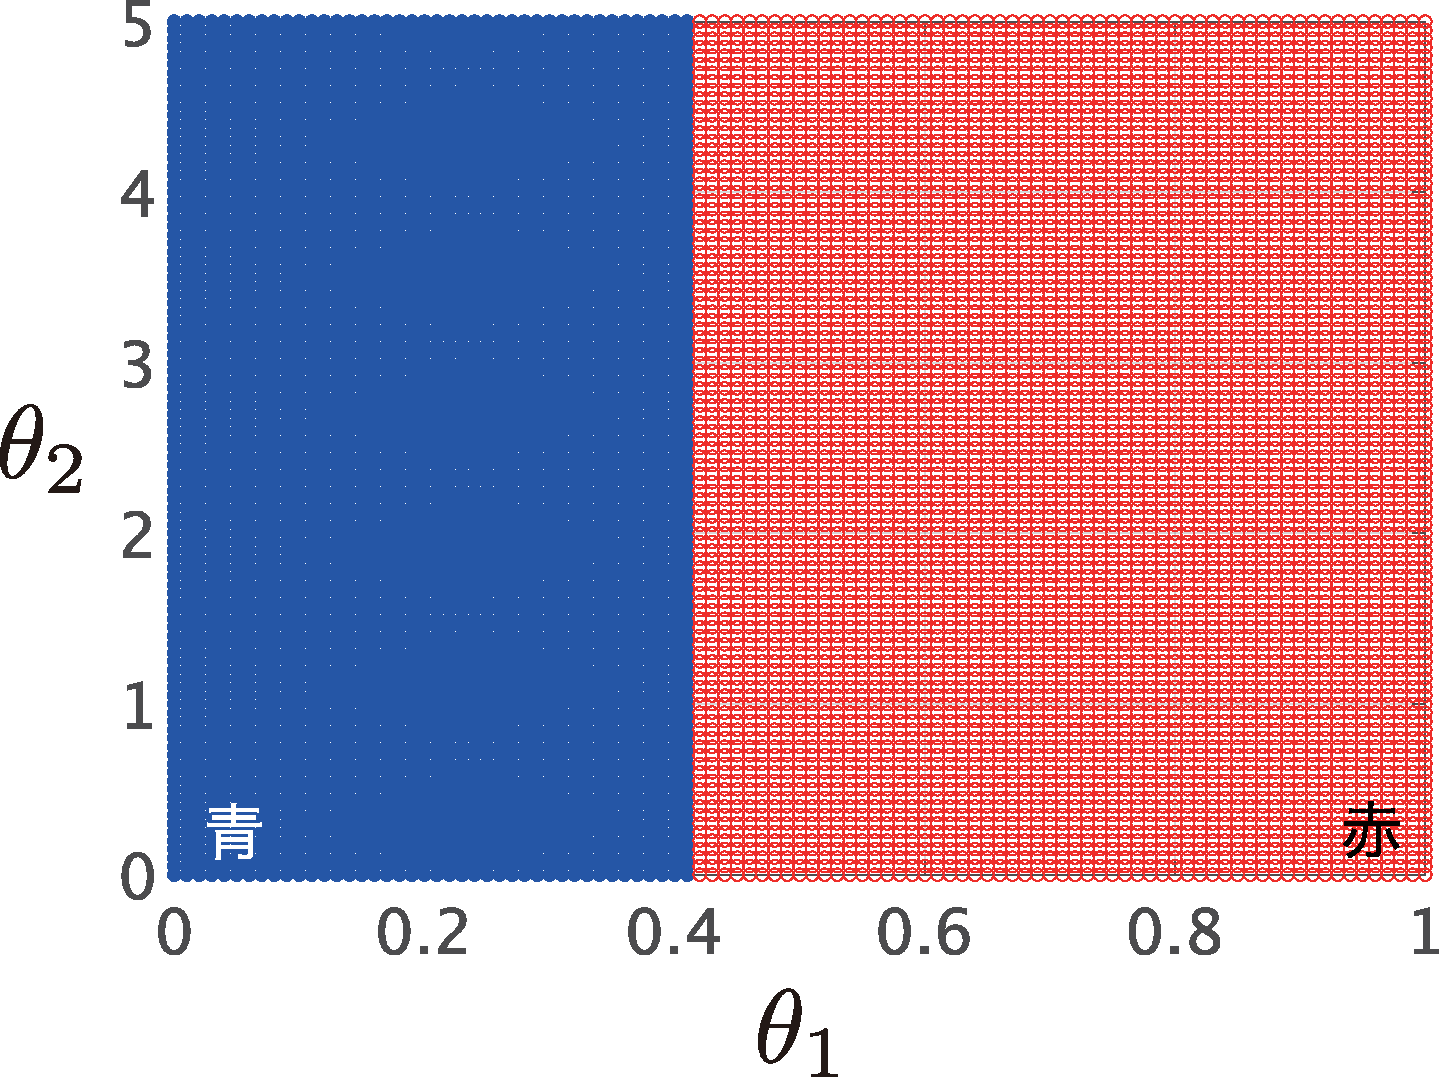
\includegraphics[width = 0.90\linewidth]{figs/Y1D1X}
    \subcaption{ $D=(10,10,10)$,$\bm{Y}=\bm{Y}_0$ }
    \medskip
  \end{minipage}
  \begin{minipage}{0.49\linewidth}
    \centering
    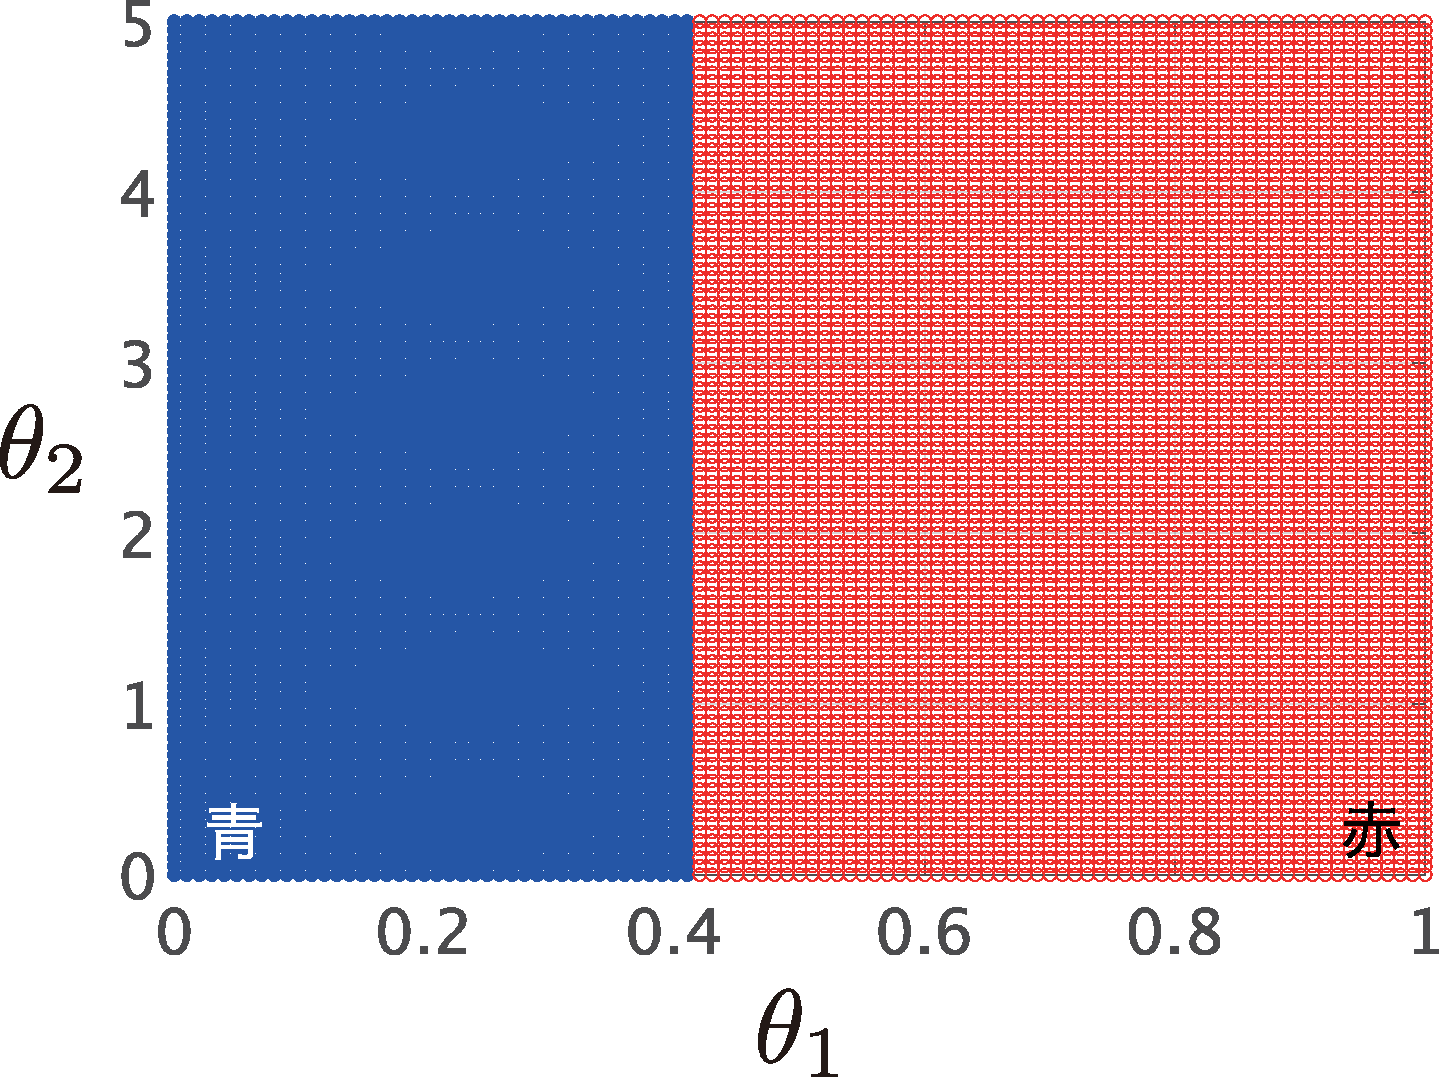
\includegraphics[width = 0.90\linewidth]{figs/Y1D0.01X}
    \subcaption{$D=(0.1,0.1,0.1)$,$\bm{Y}=\bm{Y}_0$ }
    \medskip
  \end{minipage}
}
  \centering
  {
  \begin{minipage}{0.49\linewidth}
      \centering
    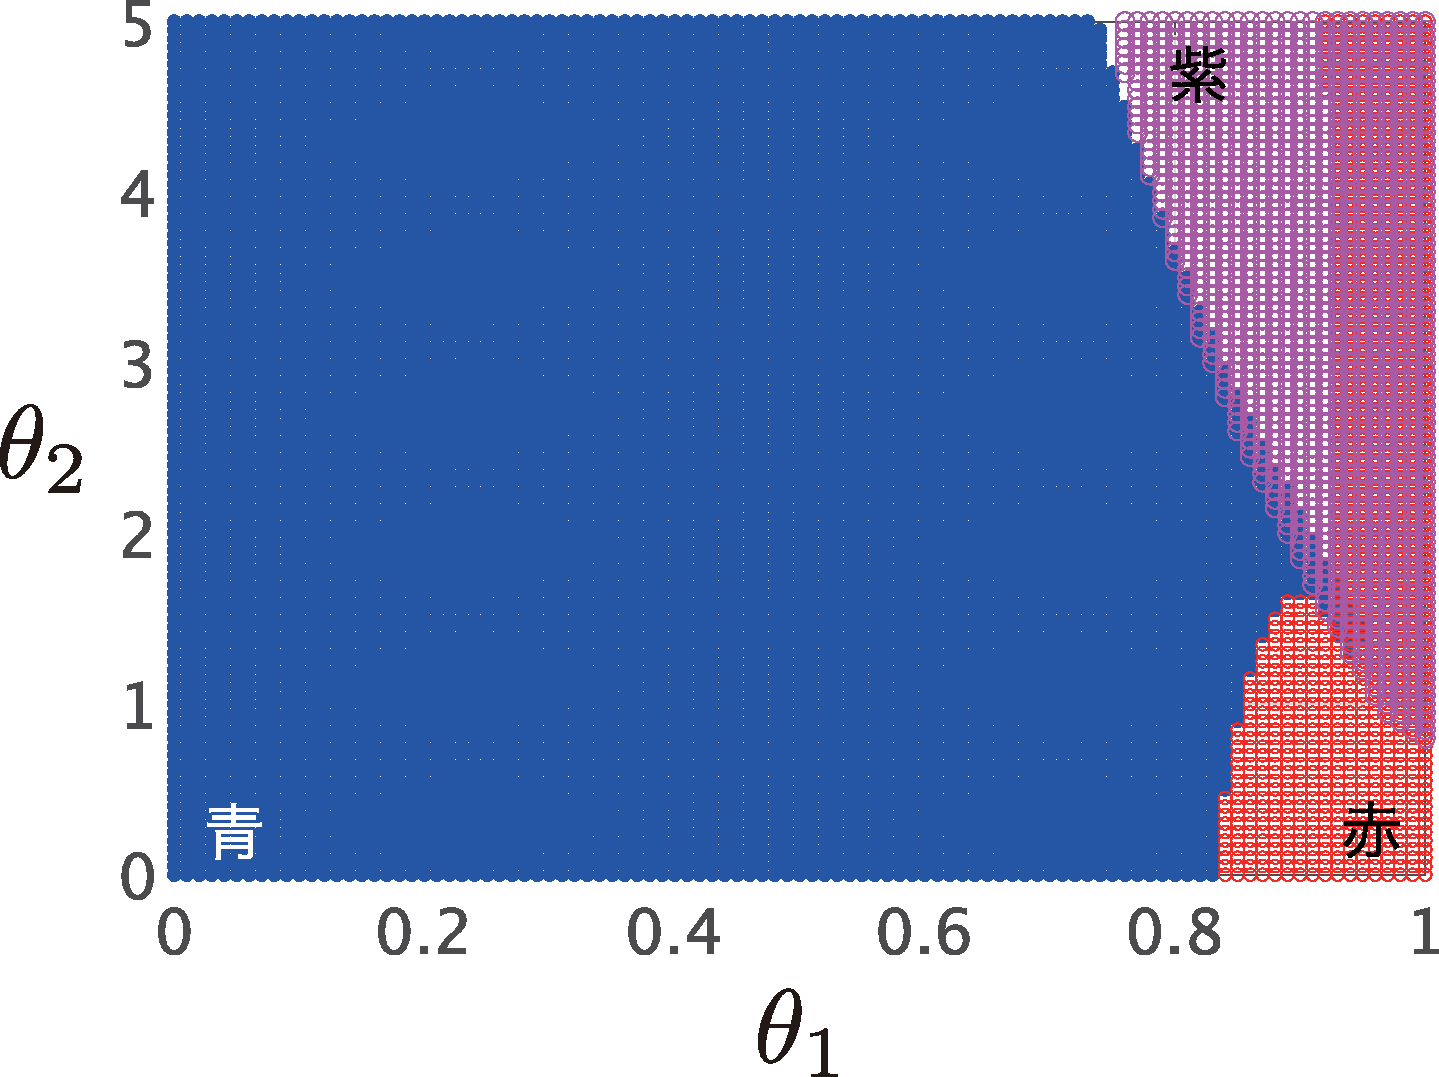
\includegraphics[width = 0.90\linewidth]{figs/Y0.01D1X}
    \subcaption{$D=(10,10,10)$,$\bm{Y}=\tfrac{\bm{Y}_0}{100}$ }
    \medskip
  \end{minipage}
  \begin{minipage}{0.49\linewidth}
    \centering
    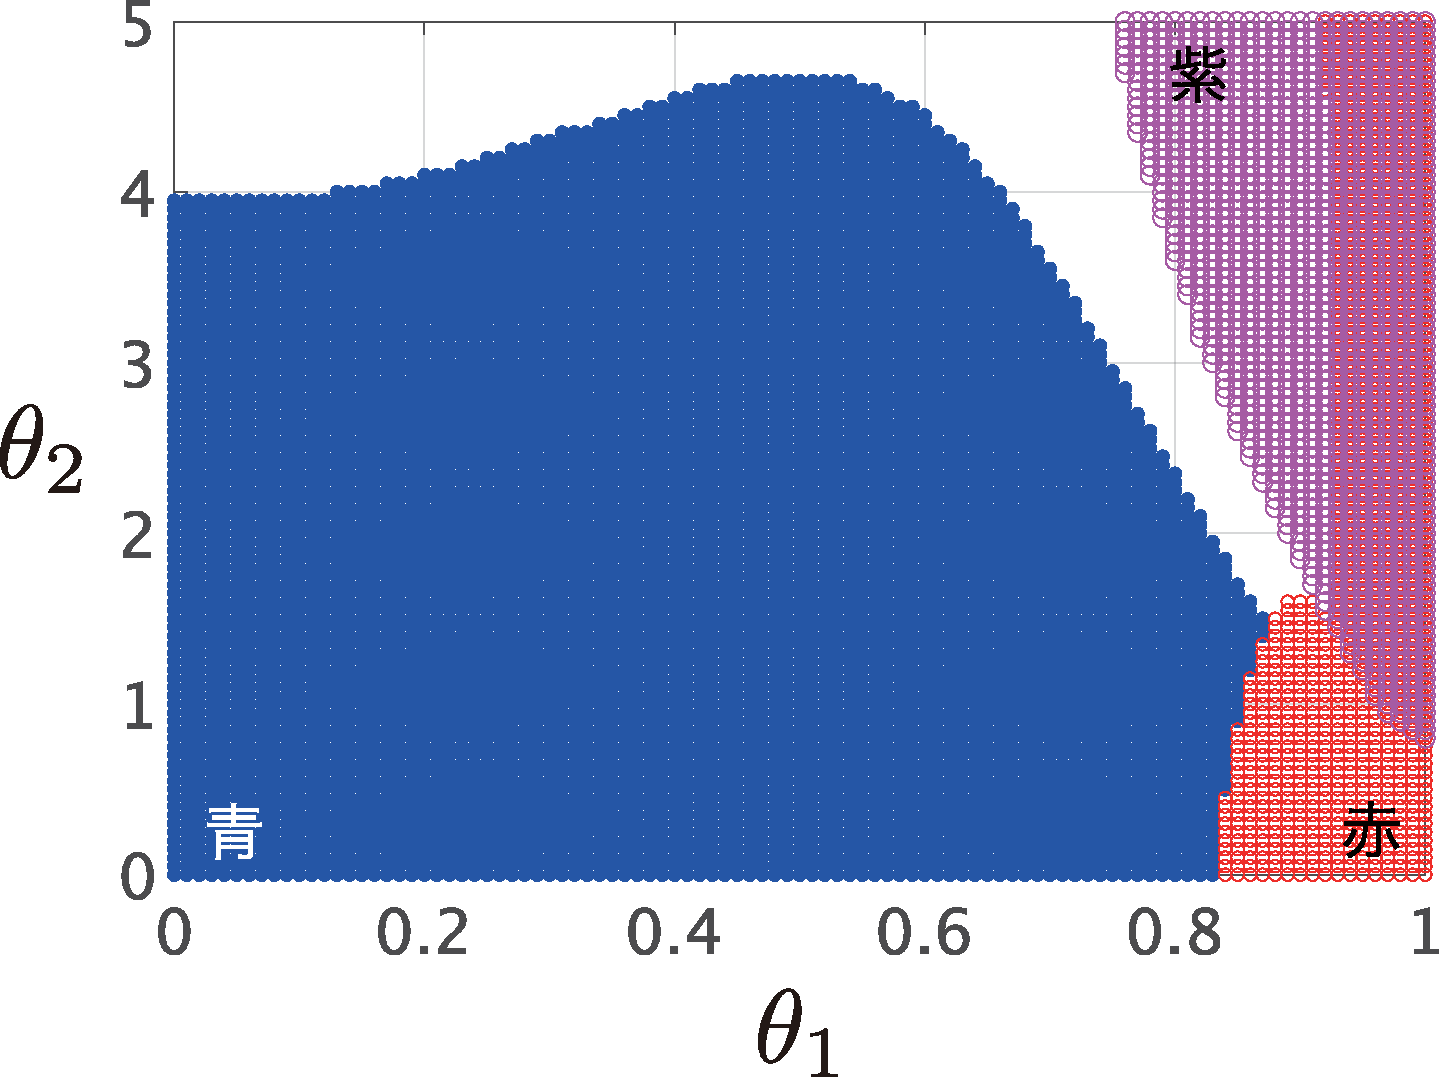
\includegraphics[width = 0.90\linewidth]{figs/Y0.01D0.01X}
    \subcaption{$D=(0.1,0.1,0.1)$,$\bm{Y}=\tfrac{\bm{Y}_0}{100}$ }
    \medskip
  \end{minipage}
}
% \medskip
 \caption{\textbf{Regions of parameters for which the approximate linear model is stable}}
 \label{fig:stacheckX}
\medskip
\end{figure}

%\bibliographystyle{myjunsrt}		% bib style
%\bibliography{reference}	% your bib database


\section*{Mathematical Supplement}
\red{Translated with DeepL}
\begin{補題}\label{lem:prlem}
Stable and square transfer function
\[
Q(s)=C(sI-A)^{-1}B + D
\]
を考える。
ただし,$(A,B)$は可制御であり,$(C,A)$は可観測であるものとする。
このとき,$Q(s)$が正実であるための必要十分条件は,
ある正定対称行列$P$が存在して
\begin{align*}%\label{eq:prlem}
\mat{
A^{\sf T}P+PA & PB-C^{\sf T} \\
B^{\sf T} P -C & -(D+D^{\sf T})
}\preceq 0
\end{align*}
が満たされることである。
\end{補題}

証明は\cite[Theorem 5.31]{antoulas2005approximation}や\cite[Theorem 3]{anderson1967system}などを参照されたい。
また,\cite{kottenstette2010relationships}では,関連する一連の結果が細かく整理されている。

\begin{補題}\label{lem:nilem}
安定かつ正方な伝達関数
\[
Q(s)=C(sI-A)^{-1}B + D
\]
を考える。
ただし,$(A,B)$は可制御であり,$(C,A)$は可観測であるものとする。
このとき,$Q(s)$が負虚であるための必要十分条件は,$D$が対称であり,かつ,
ある正定対称行列$P$が存在して
\begin{align*}
A^{\sf T}P+PA \preceq 0
,\qquad
-PA^{-1}B = C^{\sf T}
\end{align*}
が満たされることである。
\end{補題}

証明は\cite[Lemma 7]{xiong2010negative}などを参照されたい。

\end{document}
